\documentclass{book}%[book,paper=a5,jafontsize=13Q]{jlreq}

\usepackage[ipa]{luatexja-preset}
\usepackage{tcolorbox,tikz}%{graphicx,xcolor,}
\usetikzlibrary{intersections,calc,arrows.meta}
\usepackage{amsmath,amssymb,txfonts,pxfonts,bm}
\usepackage{mybook}

\graphicspath{{fig/}}

\title{吉田洋一『函数論 第2版』を読む}
\author{S}
\begin{document}

\frontmatter

\maketitle

\tableofcontents

\mainmatter

\chapter{複素数}%第1章

\begin{mysimplebox}{問1}
$|\alpha+\alpha'|\le|\alpha|+|\alpha'|$
($\alpha,\alpha'\in\C$)を計算によって示せ。
\end{mysimplebox}
\paragraph{証明}
$\alpha=a+bi$($a, b\in\R, i=\sqrt{-1}$)に対して$|\alpha|\coloneqq\sqrt{a^2+b^2}$と定義される。

$\alpha'=c+di$($c,d\in\R$)とする。

問1の不等式の左辺について定義に従って変形する。
\begin{align*}
    |\alpha+\alpha'|&=|(a+bi)+(c+di)|\\
    &=|(a+c)+(b+d)i|\\
    &=\sqrt{(a+c)^2+(b+d)^2}
\end{align*}

右辺についても変形する。
\begin{align*}
    |\alpha|+|\alpha'|=\sqrt{a^2+b^2}+\sqrt{c^2+d^2}
\end{align*}

よって、$\sqrt{(a+c)^2+(b+d)^2}\le\sqrt{a^2+b^2}+\sqrt{c^2+d^2}$を示せばよい。

この示すべき目的の式を変形していく。

両辺とも0以上であるから、示すべき式は両辺2
乗した形である以下の式に変形できる。
\begin{align*}
    (a+c)^2+(b+d)^2\le(a^2+b^2)+(c^2+d^2)+2\sqrt{(a^2+b^2)(c^2+d^2)}
\end{align*}

さらに以下のように展開して整理する。
\begin{align}
    (a^2+2ac+c^2)+(b^2+2bd+d^2)&\le (a^2+b^2)+(c^2+d^2)+2\sqrt{(a^2+b^2)(c^2+d^2)}\nonumber\\
    2ac+2bd&\le 2\sqrt{(a^2+b^2)(c^2+d^2)}\nonumber\\
    ac+bd&\le \sqrt{(a^2+b^2)(c^2+d^2)}\label{eq:cauchy-shwarz}\\
    ac+bd&\le \sqrt{a^2c^2+b^2d^2+a^2d^2+b^2c^2}\label{eq:cauchy-shwarz2}
\end{align}
この最終行の不等式(\ref{eq:cauchy-shwarz2})を示せばよいこととなる。

以下の計算をする。
\begin{align}
    &\left(\sqrt{a^2c^2+b^2d^2+a^2d^2+b^2c^2}\right)^2-(ac+bd)^2\nonumber\\
    &=a^2c^2+b^2d^2+a^2d^2+b^2c^2-(a^2c^2+b^2d^2+2abcd)\nonumber\\
    &=a^2d^2+b^2c^2-2abcd\nonumber\\
    &=(ad-bc)^2\ge0\label{eq:togo}
\end{align}
よって、
\begin{align*}
    (ac+bd)^2&\le\left(\sqrt{a^2c^2+b^2d^2+a^2d^2+b^2c^2}\right)^2\\
    |ac+bd|&\le\sqrt{a^2c^2+b^2d^2+a^2d^2+b^2c^2}\\
    ac+bd\le|ac+bd|&\le\sqrt{a^2c^2+b^2d^2+a^2d^2+b^2c^2}
\end{align*}
これで示すべき不等式は示された。(証明終)

\paragraph{別証1}
不等式(\ref{eq:cauchy-shwarz})は、よく知られたコーシー・シュワルツの不等式である。すなわち、$\bm{x}=(a,b)$、$\bm{y}=(c,d)$とすると、不等式(\ref{eq:cauchy-shwarz})は、ベクトルの内積と大きさによって、
\begin{align}
    \bm{x}\cdot \bm{y}\le|\bm{x}||\bm{y}|\label{eq:cauchy-shwarz0}
\end{align}
と書き表される。

この不等式は、$t\in\R$に対して、以下のよく知られた証明がある。すなわち、
\begin{align*}
    0\le|t\bm{x}+\bm{y}|^2
    =|\bm{x}|^2t^2+2(\bm{x}\cdot\bm{y})t+|\bm{y}|^2
\end{align*}
であるが、2次方程式$|\bm{x}|^2t^2+2(\bm{x}\cdot\bm{y})t+|\bm{y}|^2=0$の判別式$D\le 0$より
\begin{align*}
    \frac{D}{4}=(\bm{x}\cdot\bm{y})^2-|\bm{x}|^2|\bm{y}|^2\le 0
\end{align*}
よって、$\bm{x}\cdot\bm{y}\le|\bm{x}\cdot\bm{y}|\le|\bm{x}||\bm{y}|$が言える。(証明終)

\paragraph{別証2}
$\alpha=0$のとき、不等式の左辺と右辺は等しい。よって不等式は成り立つ。

$\alpha\neq 0$のとき、示すべき不等式の両辺を$|\alpha|$で割ると
\begin{align*}
    \frac{|\alpha+\alpha'|}{|\alpha|}&\le\frac{|\alpha|}{|\alpha|}+\frac{|\alpha'|}{|\alpha|}\\
    \left|\frac{\alpha+\alpha'}{\alpha}\right|&\le 1+\left|\frac{\alpha'}{\alpha}\right|\\
    \left|1+\frac{\alpha'}{\alpha}\right|&\le 1+\left|\frac{\alpha'}{\alpha}\right|
\end{align*}
よって、$\frac{\alpha'}{\alpha}$を改めて$\alpha$ととり直して、$|1+\alpha|\le 1+|\alpha|$を示せばよい。
$\alpha=a+bi$(ただし、$a,b\in\R$)のとき、
\begin{align*}
    |1+\alpha|&=|a+1+bi|=\sqrt{(a+1)^2+b^2}\\
    1+|\alpha|&=1+|a+bi|=1+\sqrt{a^2+b^2}
\end{align*}
よって
\begin{align*}
    (1+|\alpha|)^2-(|1+\alpha|)^2
    &=(1+\sqrt{a^2+b^2})^2-\{(a+1)^2+b^2\}\\
    &=1+2\sqrt{a^2+b^2}+a^2+b^2-(a^2+2a+1+b^2)\\
    &=2(\sqrt{a^2+b^2}-a)\ge 2(\sqrt{a^2}-a)
    =2(|a|-a)\ge 0
\end{align*}
(証明終)
\begin{mysimplebox}{問2}
    $z_k\in\C$($k=1,2,\dots,n$)に対して、$|z_1+z_2+\dots+z_n|\le|z_1|+|z_2|+\dots+|z_n|$であり、等号が成立するのは、$z_k$($k=1,2,\dots,n$)が$z=0$を起点とする同じ半直線の上にあるときに限ることを示せ。
\end{mysimplebox}
\paragraph{証明}
$|z_1+z_2+\dots+z_n|\le|z_1|+|z_2|+\dots+|z_n|$であることは、問1の結果と$n$に関する帰納法によって示される。

$n=2$のとき、等号が成立する条件を考える。すなわち、$|z_1+z_2|=|z_1|+|z_2|$が成り立っているとする。複素数と実2次元平面上の点を同一視して$z_1=(a,b), z_2=(c,d)$($a,b,c,d\in\R$)とすると、($\ref{eq:togo}$)式より、$ad=bc$の場合に限られることが分かる。

$a=0$の場合、$b=0$または$c=0$である。

$b=0$の場合、$z_1=(0,0)$であるから、どのような$z_2=(c,d)$に対しても$z_1, z_2$は原点を起点とする半直線上にある。

$c=0$の場合、$z_1=(0,b), z_2=(0,d)$であるが、$|z_1+z_2|=|z_1|+|z_2|$は、
\begin{align*}
    |b+d|=|b|+|d|
\end{align*}
と書き直される。これは$b$と$d$が同符号であることを表す。よって$z_1$と$z_2$は虚軸上で同じ方向を向いており、原点を起点とする半直線上にあることが分かる。

$a\neq 0$の場合、$ad=bc$より、$d=\frac{bc}{a}$である。よって
\begin{align*}
    z_2&=(c,d)=\left(c,\frac{bc}{a}\right)
    =\frac{c}{a}(a,b)=\frac{c}{a}z_1.
\end{align*}
ゆえに、$k\coloneqq\frac{c}{a}$とすると、$z_2=kz_1$である。
このとき、$|z_1|\neq 0$であり
\begin{align*}
    |z_1+z_2|&=|z_1+kz_1|
    =|(1+k)z_1|=|1+k||z_1|,\\
    |z_1|+|z_2|&=|z_1|+|kz_1|
    =|z_1|+|k||z_1|=(1+|k|)|z_1|.
\end{align*}
ここで、$k\le -1$のとき$|1+k|=-1-k\neq 1-k=1+|k|$であり不適。

また、$-1<k<0$のとき$|1+k|=1+k\neq 1-k=1+|k|$であり不適。

最後に$k\ge 0$のとき、$|1+k|=1+k=1+|k|$であり適する。

したがって$k\ge 0$である。これは$z_1$と$z_2$が同じ半直線上にあることを表す。
%$c\neq 0$であり、次の式が成り立つ。
%\begin{align*}
%    \frac{b}{a}=\frac{d}{c}=k
%\end{align*}
%これは、$z_1$と$z_2$が同一直線上にあること%を表している。
%
%さらに、
%\begin{align*}
%    |z_1+z_2|&=|(a+c)+(b+d)i|\\
%    &=|(a+c)+(ak+ck)i|\\
%    &=|a+c||1+ki|\\
%    &=|a+c|\sqrt{1+k^2}\\
%    |z_1|+|z_2|&=|a+bi|+|c+di|\\
%    &=|a+aki|+|c+cki|\\
%    &=|a||1+ki|+|c||1+ki|\\
%    &=(|a|+|c|)\sqrt{1+k^2}
%\end{align*}
%よって、$|a+c|=|a|+|c|$が成り立つ。これは$a$と$c$が同符号であることを表している。
%
%以上より、$z_1$と$z_2$は原点を起点とする半直線上にある。

逆に、$z_1$と$z_2$は原点を起点とする半直線上にあるとき、問題の不等式の等号が成立している。

したがって、$n=2$のとき、不等式の等号が成立するのは$z_1$と$z_2$が原点を起点とする半直線上にあることが示せた。

$n=3$以上のときも、帰納法によって示される。

ところで、($\ref{eq:cauchy-shwarz0}$)式において、$\bm{x}\cdot \bm{y}=|\bm{x}||\bm{y}|\cos \theta$(ただし$\theta$は$z_1$と$z_2$のなす角の大きさ)であることを知っていれば、問題の不等式の等号が成り立つのは、$|\bm{x}||\bm{y}|\cos \theta=|\bm{x}||\bm{y}|$のときであり、$\bm{x}, \bm{y}$ともに0でなければ$\cos \theta=1$となる。よって、$\theta=0$($2\pi$分の違いは無視する)であるから、不等式の等号が成立するのは、複素数平面上の点たちが原点を起点とする半直線上にあることが容易に分かる。(証明終)

\paragraph{別証}
$|z_1+z_2|=|z_1|+|z_2|$が成り立つとき、$z_1, z_2$が原点を起点とする半直線上にあることを示す。

$z_1=0$のとき、$z_1, z_2$が同じ半直線上にあることは明らかである。

$z_1\neq 0$のとき、$|z_1|\neq 0$であるから、
$|z_1+z_2|=|z_1|+|z_2|$の両辺を$|z_1|$で割ると
\begin{align*}
    \frac{|z_1+z_2|}{|z_1|}
    &=\frac{|z_1|+|z_2|}{|z_1|},\\
    \left|\frac{z_1+z_2}{z_1}\right|
    &=\left|\frac{z_1}{z_1}\right|
    +\left|\frac{z_2}{z_1}\right|,\\
    \left|1+\frac{z_2}{z_1}\right|
    &=1
    +\left|\frac{z_2}{z_1}\right|.
\end{align*}
よって$z\coloneqq \frac{z_2}{z_1}$とおけば、
$|1+z|=1+|z|$が成り立つとき、$z$が実軸の非負の部分にあることを示せばよい。両辺2乗すると
\begin{align*}
    |1+z|^2&=(1+|z|)^2,\\
    (1+z)(1+\overline{z})&=1+2|z|+|z|^2,\\
    1+z+\overline{z}+z\overline{z}&=1+2|z|+|z|^2,\\
    z+\overline{z}&=2|z|\\
    \Re z&=|z|.
\end{align*}
これは$z$が非負の実数であることを示している。(証明終)

\begin{mysimplebox}{問3}
    $|\alpha|<1$のとき、$|z|<1$ならば$\left|\frac{z-\alpha}{\bar{\alpha}z-1}\right|<1$であり、$|z|=1$ならば$\left|\frac{z-\alpha}{\bar{\alpha}z-1}\right|=1$であることを示せ。
\end{mysimplebox}
\paragraph{証明}
$\alpha=a+bi, z=c+di$($a,b,c,d\in\R$)とする。

\begin{align*}
    |\bar{\alpha}z-1|&=|(a-bi)(c+di)-1|\\
    &=|(ac+bd-1)+(ad-bc)i|\\
    &=\sqrt{(ac+bd-1)^2+(ad-bc)^2}\\
    &=\sqrt{(a^2c^2+b^2d^2+1+2abcd-2bd-2ac)+(a^2d^2-2abcd+b^2c^2)}\\
    &=\sqrt{a^2c^2+b^2d^2-2bd-2ac+a^2d^2+b^2c^2+1}\\
    &=\sqrt{(a^2+b^2)(c^2+d^2)-2(ac+bd)+1}\\
    |z-\alpha|&=|(c-a)+(d-b)i|\\
    &=\sqrt{(c-a)^2+(d-b)^2}\\
    &=\sqrt{a^2+b^2+c^2+d^2-2(ac+bd)}
\end{align*}
よって、
\begin{align*}
    &|\bar{\alpha}z-1|^2-|z-\alpha|^2\\
    =&(a^2+b^2)(c^2+d^2)-(a^2+b^2)-(c^2+d^2)+1\\
    =&\{(a^2+b^2)-1\}\{(c^2+d^2)-1\}
\end{align*}

$|\alpha|<1$ならば$(a^2+b^2)-1<0$、$|z|<1$ならば$(c^2+d^2)-1<0$である。
よって、
\begin{align*}
    &|\bar{\alpha}z-1|^2-|z-\alpha|^2>0\\
    &|\bar{\alpha}z-1|^2>|z-\alpha|^2\\
    &|\bar{\alpha}z-1|>|z-\alpha|\\
    &\left|\frac{z-\alpha}{\bar{\alpha}z-1}\right|<1
\end{align*}

また、$|z|=1$ならば$(c^2+d^2)-1=0$であるから、上記と同じ計算で等号が成り立ち、
\begin{align*}
    &\left|\frac{z-\alpha}{\bar{\alpha}z-1}\right|=1
\end{align*}
が言える。(証明終)

\paragraph{別証1}

図形的に解くこともできる。

$\arg\bar{\alpha}z-\arg 1=\arg\bar{\alpha}+\arg z-0=-\arg\alpha+\arg z$であるから、3点$\bar{\alpha}z$,O,1がなす角度と、3点$z$,O,$\alpha$がなす角度は等しい。その大きさを$\theta$とすると、余弦定理により、
\begin{align*}
    |z-\alpha|^2&=|z|^2+|\alpha|^2-2|z||\alpha|\cos\theta\\
    |\bar{\alpha}z-1|^2&=|\bar{\alpha}z|^2+1^2-2|\bar{\alpha}z|\cos\theta\\
    &=|\alpha|^2|z|^2+1-2|z||\alpha|\cos\theta
\end{align*}
よって、
\begin{align*}
    |\bar{\alpha}z-1|^2-|z-\alpha|^2&=|\alpha|^2|z|^2-|z|^2-|\alpha|^2+1\\
    &=(|z|^2-1)(|\alpha|^2-1)
\end{align*}
ゆえに、$|\alpha|<1, |z|<1$のとき、 $|\bar{\alpha}z-1|^2-|z-\alpha|^2>0$となり、上記と同じ結論を得る。(証明終)
\begin{figure}
    \centering
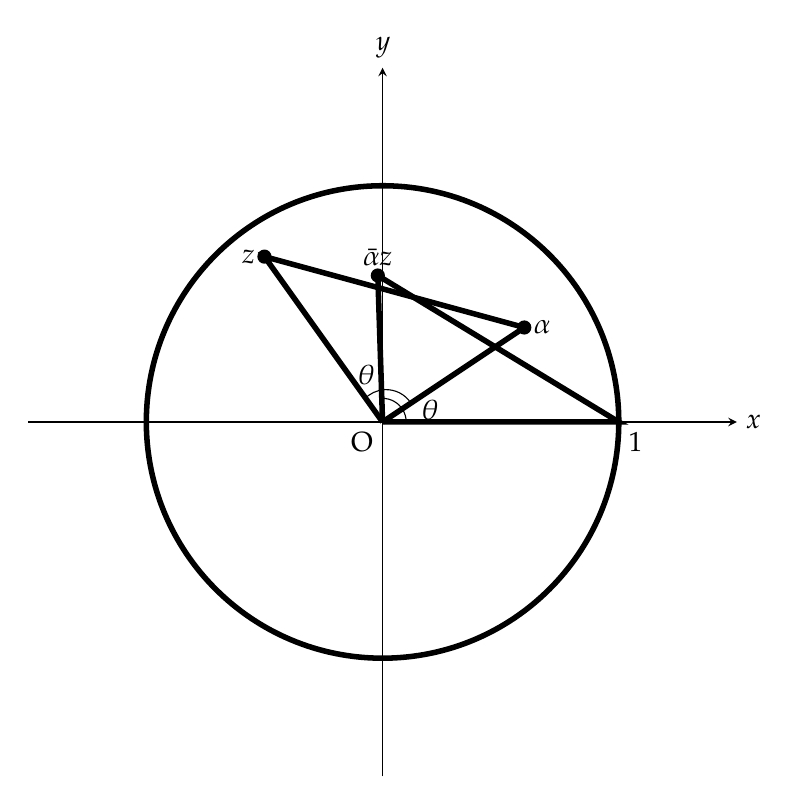
\begin{tikzpicture}[x=30mm,y=30mm,domain=-1.5:1.5,samples=200,>=stealth]
    \draw[->](-1.5,0)--(1.5,0) node[right]{$x$};
    \draw[->](0,-1.5)--(0,1.5) node[above]{$y$};
    \draw (0,0) node[below left]{O};
    \draw[line width=2pt] (0,0) circle (1);
    \fill[black] (-0.5,0.7) circle (0.03) node[left] {$z$}
                 (0.6,0.4) circle (0.03) node[right] {$\alpha$}
                 (-0.02,0.62) circle (0.03) node[above]{$\bar{\alpha}z$};
    \draw (1,0) node[below right] {1};
    \draw[line width=2pt] (0,0)--(-0.5,0.7)--(0.6,0.4)--(0,0);
    \draw[line width=2pt] (0,0)--(-0.02,0.62)--(1,0)--(0,0);
    \draw (0.1,0) arc (0:92:0.1);
    \draw (0.2,0.05) node {$\theta$};
    \draw (0.12,0.08) arc (33:138:0.125);
    \draw (-0.07,0.2) node {$\theta$};
\end{tikzpicture}
\caption{問3の図形的解法}
\end{figure}

\paragraph{別証2}
複素数の計算規則によって、
\begin{align*}
    |\bar{\alpha}z-1|^2-|z-\alpha|^2
    &=(\bar{\alpha}z-1)(\alpha\bar{z}-1)-(z-\alpha)(\bar{z}-\bar{\alpha})\\
    &=|\alpha|^2|z|^2-\bar{\alpha}z-\alpha\bar{z}+1-(|z|^2-\bar{\alpha}z-\alpha\bar{z}+|\alpha|^2)\\
    &=|\alpha|^2|z|^2-|z|^2-|\alpha|^2+1\\
    &=(|z|^2-1)(|\alpha|^2-1)
\end{align*}
と計算でき、上記と同様の結論を得る。(証明終)

\begin{mysimplebox}{問4(Cauchy--Hadamard)}
    $\sum_{n=0}^\infty c_nz^n=c_0+c_1z+\dots+c_nz^n+\dots$(①)の形の級数を$z$の\textgt{整級数}という。
    \[\overline{\lim_{n\to\infty}}|c_n|^{\frac{1}{n}}=\left\{\begin{array}{lll}
      \lambda  \,(0<\lambda<+\infty) & \mbox{ならば} & R=\frac{1}{\lambda}\\
      0 & \mbox{ならば} & R=+\infty\\
      +\infty & \mbox{ならば} & R=0
    \end{array}\right.\]
    として$R$を定めるとき、$\sum_{n=0}^\infty c_nz^n$は$|z|<R$ならば絶対収束し、$|z|>R$ならば発散する。このことを示せ。
\end{mysimplebox}
\paragraph{証明}
$0<\lambda<+\infty$の場合は本で証明が済んでいるので省略する。

まずは$\displaystyle\overline{\lim_{n\to\infty}}|c_n|^{\frac{1}{n}}=0$のときを考える。整級数①が$|z|<+\infty$で絶対収束することを示せばよい。

$|z|<\frac{1-\delta}{\delta}$を満たす$\delta\,(0<\delta<1)$が存在する。

$\displaystyle\overline{\lim_{n\to\infty}}|c_n|^{\frac{1}{n}}=0$であるから、十分大きい$n$に対して$|c_n|^\frac{1}{n}<\delta$となる。

よって、
\begin{align*}
    |c_nz^n|&=\left(|c_n|^\frac{1}{n}\right)^n|z|^n<\delta^n\left(\frac{1-\delta}{\delta}\right)^n
    =(1-\delta)^n.
\end{align*}
ゆえに、
\begin{align*}
    \sum_{k=n}^\infty |c_kz^k|&<\sum_{k=n}^\infty(1-\delta)^k
\end{align*}
$0<1-\delta<1$であるから、上式の左辺は等比級数として収束する。したがって、$\sum_{k=n}^\infty |c_kz^k|$も収束する。すなわち、整級数①は絶対収束する。

次に$\displaystyle\overline{\lim_{n\to\infty}}|c_n|^{\frac{1}{n}}=+\infty$のときを考える。

$|z|>0$ならば整級数①が発散することを示せばよい。

$|z|>0$とすると、$|z|>\frac{1}{\delta}>0$となる$\delta\,(>0)$が存在する。
また条件より、十分大きい$n$に対して、$|c_n|^\frac{1}{n}>\delta$となる$n$が無数に存在する。
よって、
\begin{align*}
    |c_nz^n|&=\left(|c_n|^\frac{1}{n}\right)^n|z|^n>\delta^n\left(\frac{1}{\delta}\right)^n
    =1
\end{align*}
となる$n$が無数に存在する。

ゆえに、$|c_nz^n|\to 0$でないため、整級数①は発散する。(証明終)

この問題からも分かったことだが、級数の収束の判定法の1つは、等比級数と比較することである。

上記で定めた$R$を整級数①の\textgt{収束半径}という。

\paragraph{補足}
上記証明中の$\displaystyle\overline{\lim_{n\to\infty}}|c_n|^{\frac{1}{n}}=0$の場合とは結局$\displaystyle{\lim_{n\to\infty}|c_n|^{\frac{1}{n}}=0}$ということである。

\begin{mysimplebox}{問5}
    $\sum_{n=0}^\infty c_nz^n$が$z=z_0$で収束すれば$|z|<|z_0|$であるような$z$に対しては絶対収束することを示せ。
\end{mysimplebox}
\paragraph{証明}
本にも書いてあるとおり、これは言い換えると、「$\sum_{n=0}^\infty c_nz^n$が$z=z_1$で絶対収束しなければ$|z|>|z_1|$であるような$z$に対しては発散する」ということである。この言い換えた方を示す。

$\sum_{n=0}^\infty c_nz^n$が$z=z_1$で絶対収束しなければ、収束半径$R$は、$R<|z_1|$である。よって、$|z|>|z_1|>R$では、$\sum_{n=0}^\infty c_nz^n$は発散する。(証明終)

\begin{mysimplebox}{問6}
    $c_n\neq 0\,(n=k, k+1, k+2,\dots)$、$R=\lim_{n\to\infty}|c_nc_{n+1}^{-1}|$ならば、$\sum_{n=0}^\infty c_nz^n$の収束半径は$R$であることを示せ。
\end{mysimplebox}
\paragraph{証明}
$R=\lim_{n\to\infty}|c_nc_{n+1}^{-1}|$であることより、$0<\epsilon<R$である任意の数$\epsilon$に対して、ある正数$N$が存在し、$n>N$となる任意の$n$に対して、
\begin{align*}
    R-\epsilon<\left|\frac{c_n}{c_{n+1}}\right|<R+\epsilon
\end{align*}
となる。よって、
\begin{align*}
    \frac{|c_n|}{R+\epsilon}<|c_{n+1}|<\frac{|c_n|}{R-\epsilon}
\end{align*}    
である。

ゆえに、$k>0$に対して、
\begin{align}
    |c_{n+k}|&>\frac{|c_{n+k-1}|}{R+\epsilon}>\frac{|c_{n+k-2}|}{(R+\epsilon)^2}>\dots>\frac{|c_{n}|}{(R+\epsilon)^k},\label{eq:convR1}\\
    |c_{n+k}|&<\frac{|c_{n+k-1}|}{R-\epsilon}<\frac{|c_{n+k-2}|}{(R-\epsilon)^2}<\dots<\frac{|c_{n}|}{(R-\epsilon)^k}.\label{eq:convR2}
\end{align}

したがって、
\begin{align*}
    \left\{\frac{|c_{n}|}{(R+\epsilon)^k}\right\}^\frac{1}{n+k}<&|c_{n+k}|^\frac{1}{n+k}< \left\{\frac{|c_{n}|}{(R-\epsilon)^k}\right\}^\frac{1}{n+k}\\
    \frac{|c_{n}|^\frac{1}{n+k}}{(R+\epsilon)^\frac{k}{n+k}}<&|c_{n+k}|^\frac{1}{n+k}< \frac{|c_{n}|^\frac{1}{n+k}}{(R-\epsilon)^\frac{k}{n+k}}
\end{align*}
ここで、$k\longrightarrow\infty$の極限において、
\begin{align*}
    \frac{|c_{n}|^\frac{1}{n+k}}{(R+\epsilon)^\frac{k}{n+k}}&\longrightarrow \frac{|c_{n}|^0}{(R+\epsilon)^1}=\frac{1}{R+\epsilon},\\
    \frac{|c_{n}|^\frac{1}{n+k}}{(R-\epsilon)^\frac{k}{n+k}}&\longrightarrow \frac{|c_{n}|^0}{(R-\epsilon)^1}=\frac{1}{R-\epsilon}.
\end{align*}
よって、
\begin{align*}
    \frac{1}{R+\epsilon}<\lim_{k\to\infty}|c_{n+k}|^\frac{1}{n+k}<\frac{1}{R-\epsilon}.
\end{align*}
$\epsilon$はいくらでも小さくとれるから、
\begin{align*}
    \lim_{k\to\infty}|c_{n+k}|^\frac{1}{n+k}=\frac{1}{R}
\end{align*}
したがって、Cauchy--Hadamardの定理により、$\sum_{n=0}^\infty c_nz^n$の収束半径は$R$である。(証明終)

\paragraph{別証}
Cauchy--Hadamardの定理を使わず、$R$が収束半径であることを直接示す。

$0<\epsilon<\frac{R}{2}$である$\epsilon$に対して、$(\ref{eq:convR1}),(\ref{eq:convR2})$式が成り立っているとする。

まずは$|z|<R-2\epsilon$のときを考える。
$(\ref{eq:convR2})$式から、
\begin{align*}
    \sum_{k=0}^\infty |c_{n+k}z^{n+k}|
    <\sum_{k=0}^\infty \frac{|c_n|(R-2\epsilon)^{n+k}}{(R-\epsilon)^k}=|c_n|(R-2\epsilon)^n\sum_{k=0}^\infty \left(\frac{R-2\epsilon}{R-\epsilon}\right)^k
\end{align*}
$0<\frac{R-2\epsilon}{R-\epsilon}<1$であるから、$\sum_{n=0}^\infty c_nz^n$は絶対収束する。

次に$|z|>R+2\epsilon$のときを考える。
$(\ref{eq:convR1})$式から、
\begin{align*}
    \sum_{k=0}^\infty |c_{n+k}z^{n+k}|
    >\sum_{k=0}^\infty \frac{|c_n|(R+2\epsilon)^{n+k}}{(R+\epsilon)^k}=|c_n|(R+2\epsilon)^n\sum_{k=0}^\infty \left(\frac{R+2\epsilon}{R+\epsilon}\right)^k
\end{align*}
$1<\frac{R+2\epsilon}{R+\epsilon}$であるから、$\sum_{n=0}^\infty c_nz^n$は発散する。

よって、$\sum_{n=0}^\infty c_nz^n$の収束半径$r$は、$R-2\epsilon<r<R+2\epsilon$を満たす。$\epsilon$は$0<\epsilon<\frac{R}{2}$の範囲で任意であるから、$r=R$である。(証明終)

\begin{mysimplebox}{問7}
    次の整級数の収束半径を求めよ。
    \begin{itemize}
        \item[(i)]{$\displaystyle\sum_{n=0}^{\infty}\frac{z^n}{n^n}$}
        \item[(ii)]{$\displaystyle\sum_{n=0}^{\infty}n!z^n$}
        \item[(iii)]{$\displaystyle 1+\sum_{n=1}^{\infty}\frac{\alpha(\alpha+1)(\alpha+2)\dots(\alpha+n-1)\beta(\beta+1)\dots(\beta+n-1)}{n!\gamma(\gamma+1)(\gamma+2)\dots(\gamma+n-1)}z^n$\\($\gamma\neq 0, -1,-2,-3,\dots$)[超幾何級数]} 
    \end{itemize}
\end{mysimplebox}
問6の結果を使うと計算できる。

(i)について。
\begin{align*}
    &c_n=\frac{1}{n^n}\\
    &\frac{c_n}{c_{n+1}}=\frac{(n+1)^{n+1}}{n^n}=\left(\frac{n+1}{n}\right)^n(n+1)=\left(1+\frac{1}{n}\right)^n(n+1)\overset{n\longrightarrow\infty}{\longrightarrow}e\cdot \infty=\infty
\end{align*}
よって、収束半径は$+\infty$である。すなわち、任意の$z\in\C$で収束する。

(ii)について。
\begin{align*}
    &c_n=n!\\
    &\frac{c_n}{c_{n+1}}=\frac{n!}{(n+1)!}=\frac{1}{n+1}\overset{n\longrightarrow\infty}{\longrightarrow}0
\end{align*}
よって、収束半径は0である。

(iii)
$n>1$とする。また、$\alpha, \beta\neq 0, -1,-2,-3,\dots$とする。
\begin{align*}
    &c_n=\frac{\alpha(\alpha+1)(\alpha+2)\dots(\alpha+n-1)\beta(\beta+1)\dots(\beta+n-1)}{n!\gamma(\gamma+1)(\gamma+2)\dots(\gamma+n-1)}\\
    &\frac{c_n}{c_{n+1}}=\frac{(n+1)(\gamma+n)}{(\alpha+n)(\beta+n)}=\frac{(1+\frac{1}{n})(\frac{\gamma}{n}+1)}{(\frac{\alpha}{n}+1)(\frac{\beta}{n}+1)}\overset{n\longrightarrow\infty}{\longrightarrow}1
\end{align*}
よって、収束半径は1である。

ただし、$\alpha$と$\beta$のどちらかが0または負の整数であるとき、(iii)の整級数は有限次数であるため、収束半径は$+\infty$である。

\paragraph{別解}
Cauchy--Hadamardの定理によって収束半径を求めるてみる。

(i)については、
\begin{align*}
    \overline{\lim_{n\to\infty}}|c_n|^\frac{1}{n}=\overline{\lim_{n\to\infty}}\left(\frac{1}{n^n}\right)^\frac{1}{n}=\overline{\lim_{n\to\infty}}\frac{1}{n}=0
\end{align*}
よって収束半径が$+\infty$であることが分かる。

(ii)については、対数をとって考える。すなわち、
\begin{align*}
    \log |c_n|^\frac{1}{n}
   &=\log n!^\frac{1}{n}
   =\frac{\log 1 +\log 2 +\dots+\log n}{n}\\
   &>\frac{\int_{1}^{n+1}\log x dx}{n}
   =\frac{\left[x\log x -x\right]_1^{n+1}}{n}
   =\frac{(n+1)\log(n+1)-(n+1)-(-1)}{n}\\
   &=\frac{(n+1)\log(n+1)-n}{n}
   =\left(1+\frac{1}{n}\right)\log(n+1)-1
   \overset{n\longrightarrow\infty}{\longrightarrow}\infty
\end{align*}
\begin{figure}
    \centering
    \scalebox{0.6}{% Created by tikzDevice version 0.12.5 on 2023-10-09 15:35:09
% !TEX encoding = UTF-8 Unicode
\begin{tikzpicture}[x=1pt,y=1pt]
\definecolor{fillColor}{RGB}{255,255,255}
\path[use as bounding box,fill=fillColor,fill opacity=0.00] (0,0) rectangle (505.89,361.35);
\begin{scope}
\path[clip] ( 49.20, 61.20) rectangle (480.69,312.15);
\definecolor{drawColor}{RGB}{0,0,255}

\path[draw=drawColor,line width= 0.4pt,line join=round,line cap=round] ( 69.18,-91.51) --
	( 73.17,-42.74) --
	( 77.17,-14.21) --
	( 81.16,  6.03) --
	( 85.16, 21.73) --
	( 89.15, 34.55) --
	( 93.15, 45.40) --
	( 97.14, 54.79) --
	(101.14, 63.08) --
	(105.13, 70.49) --
	(109.13, 77.20) --
	(113.12, 83.32) --
	(117.12, 88.95) --
	(121.11, 94.17) --
	(125.11, 99.02) --
	(129.11,103.56) --
	(133.10,107.83) --
	(137.10,111.85) --
	(141.09,115.65) --
	(145.09,119.26) --
	(149.08,122.70) --
	(153.08,125.97) --
	(157.07,129.10) --
	(161.07,132.09) --
	(165.06,134.96) --
	(169.06,137.72) --
	(173.05,140.38) --
	(177.05,142.94) --
	(181.04,145.40) --
	(185.04,147.79) --
	(189.03,150.10) --
	(193.03,152.33) --
	(197.03,154.50) --
	(201.02,156.60) --
	(205.02,158.64) --
	(209.01,160.62) --
	(213.01,162.55) --
	(217.00,164.42) --
	(221.00,166.25) --
	(224.99,168.03) --
	(228.99,169.77) --
	(232.98,171.46) --
	(236.98,173.12) --
	(240.97,174.74) --
	(244.97,176.32) --
	(248.96,177.86) --
	(252.96,179.38) --
	(256.95,180.86) --
	(260.95,182.31) --
	(264.94,183.73) --
	(268.94,185.12) --
	(272.94,186.49) --
	(276.93,187.83) --
	(280.93,189.14) --
	(284.92,190.44) --
	(288.92,191.70) --
	(292.91,192.95) --
	(296.91,194.17) --
	(300.90,195.38) --
	(304.90,196.56) --
	(308.89,197.72) --
	(312.89,198.86) --
	(316.88,199.99) --
	(320.88,201.10) --
	(324.87,202.19) --
	(328.87,203.26) --
	(332.86,204.32) --
	(336.86,205.36) --
	(340.86,206.39) --
	(344.85,207.40) --
	(348.85,208.40) --
	(352.84,209.39) --
	(356.84,210.36) --
	(360.83,211.31) --
	(364.83,212.26) --
	(368.82,213.19) --
	(372.82,214.11) --
	(376.81,215.02) --
	(380.81,215.91) --
	(384.80,216.80) --
	(388.80,217.67) --
	(392.79,218.54) --
	(396.79,219.39) --
	(400.78,220.23) --
	(404.78,221.06) --
	(408.77,221.89) --
	(412.77,222.70) --
	(416.77,223.50) --
	(420.76,224.30) --
	(424.76,225.09) --
	(428.75,225.86) --
	(432.75,226.63) --
	(436.74,227.39) --
	(440.74,228.14) --
	(444.73,228.89) --
	(448.73,229.63) --
	(452.72,230.36) --
	(456.72,231.08) --
	(460.71,231.79) --
	(464.71,232.50);
\end{scope}
\begin{scope}
\path[clip] (  0.00,  0.00) rectangle (505.89,361.35);
\definecolor{drawColor}{RGB}{0,0,0}

\path[draw=drawColor,line width= 0.4pt,line join=round,line cap=round] ( 65.18, 61.20) -- (464.71, 61.20);

\path[draw=drawColor,line width= 0.4pt,line join=round,line cap=round] ( 65.18, 61.20) -- ( 65.18, 55.20);

\path[draw=drawColor,line width= 0.4pt,line join=round,line cap=round] (145.09, 61.20) -- (145.09, 55.20);

\path[draw=drawColor,line width= 0.4pt,line join=round,line cap=round] (224.99, 61.20) -- (224.99, 55.20);

\path[draw=drawColor,line width= 0.4pt,line join=round,line cap=round] (304.90, 61.20) -- (304.90, 55.20);

\path[draw=drawColor,line width= 0.4pt,line join=round,line cap=round] (384.80, 61.20) -- (384.80, 55.20);

\path[draw=drawColor,line width= 0.4pt,line join=round,line cap=round] (464.71, 61.20) -- (464.71, 55.20);

\node[text=drawColor,anchor=base,inner sep=0pt, outer sep=0pt, scale=  1.00] at ( 65.18, 39.60) {0};

\node[text=drawColor,anchor=base,inner sep=0pt, outer sep=0pt, scale=  1.00] at (145.09, 39.60) {2};

\node[text=drawColor,anchor=base,inner sep=0pt, outer sep=0pt, scale=  1.00] at (224.99, 39.60) {4};

\node[text=drawColor,anchor=base,inner sep=0pt, outer sep=0pt, scale=  1.00] at (304.90, 39.60) {6};

\node[text=drawColor,anchor=base,inner sep=0pt, outer sep=0pt, scale=  1.00] at (384.80, 39.60) {8};

\node[text=drawColor,anchor=base,inner sep=0pt, outer sep=0pt, scale=  1.00] at (464.71, 39.60) {10};

\path[draw=drawColor,line width= 0.4pt,line join=round,line cap=round] ( 49.20, 70.49) -- ( 49.20,281.57);

\path[draw=drawColor,line width= 0.4pt,line join=round,line cap=round] ( 49.20, 70.49) -- ( 43.20, 70.49);

\path[draw=drawColor,line width= 0.4pt,line join=round,line cap=round] ( 49.20,105.67) -- ( 43.20,105.67);

\path[draw=drawColor,line width= 0.4pt,line join=round,line cap=round] ( 49.20,140.85) -- ( 43.20,140.85);

\path[draw=drawColor,line width= 0.4pt,line join=round,line cap=round] ( 49.20,176.03) -- ( 43.20,176.03);

\path[draw=drawColor,line width= 0.4pt,line join=round,line cap=round] ( 49.20,211.21) -- ( 43.20,211.21);

\path[draw=drawColor,line width= 0.4pt,line join=round,line cap=round] ( 49.20,246.39) -- ( 43.20,246.39);

\path[draw=drawColor,line width= 0.4pt,line join=round,line cap=round] ( 49.20,281.57) -- ( 43.20,281.57);

\node[text=drawColor,rotate= 90.00,anchor=base,inner sep=0pt, outer sep=0pt, scale=  1.00] at ( 34.80, 70.49) {0.0};

\node[text=drawColor,rotate= 90.00,anchor=base,inner sep=0pt, outer sep=0pt, scale=  1.00] at ( 34.80,105.67) {0.5};

\node[text=drawColor,rotate= 90.00,anchor=base,inner sep=0pt, outer sep=0pt, scale=  1.00] at ( 34.80,140.85) {1.0};

\node[text=drawColor,rotate= 90.00,anchor=base,inner sep=0pt, outer sep=0pt, scale=  1.00] at ( 34.80,176.03) {1.5};

\node[text=drawColor,rotate= 90.00,anchor=base,inner sep=0pt, outer sep=0pt, scale=  1.00] at ( 34.80,211.21) {2.0};

\node[text=drawColor,rotate= 90.00,anchor=base,inner sep=0pt, outer sep=0pt, scale=  1.00] at ( 34.80,246.39) {2.5};

\node[text=drawColor,rotate= 90.00,anchor=base,inner sep=0pt, outer sep=0pt, scale=  1.00] at ( 34.80,281.57) {3.0};

\path[draw=drawColor,line width= 0.4pt,line join=round,line cap=round] ( 49.20, 61.20) --
	(480.69, 61.20) --
	(480.69,312.15) --
	( 49.20,312.15) --
	cycle;
\end{scope}
\begin{scope}
\path[clip] (  0.00,  0.00) rectangle (505.89,361.35);
\definecolor{drawColor}{RGB}{0,0,0}

\node[text=drawColor,anchor=base,inner sep=0pt, outer sep=0pt, scale=  1.00] at (264.94, 15.60) {x};

\node[text=drawColor,rotate= 90.00,anchor=base,inner sep=0pt, outer sep=0pt, scale=  1.00] at ( 10.80,186.67) {log(x)};
\end{scope}
\begin{scope}
\path[clip] ( 49.20, 61.20) rectangle (480.69,312.15);
\definecolor{drawColor}{RGB}{0,0,0}

\path[draw=drawColor,line width= 0.4pt,line join=round,line cap=round] ( 65.18, 70.49) --
	(105.13, 70.49) --
	(105.13,119.26) --
	(145.09,119.26) --
	(145.09,147.79) --
	(185.04,147.79) --
	(185.04,168.03) --
	(224.99,168.03) --
	(224.99,183.73) --
	(264.94,183.73) --
	(264.94,196.56) --
	(304.90,196.56) --
	(304.90,207.40) --
	(344.85,207.40) --
	(344.85,216.80) --
	(384.80,216.80) --
	(384.80,225.09) --
	(424.76,225.09) --
	(424.76,232.50);
\end{scope}
\begin{scope}
\path[clip] (  0.00,  0.00) rectangle (505.89,361.35);
\definecolor{drawColor}{RGB}{0,0,0}

\path[draw=drawColor,line width= 0.4pt,line join=round,line cap=round] ( 65.18, 61.20) -- (464.71, 61.20);

\path[draw=drawColor,line width= 0.4pt,line join=round,line cap=round] ( 65.18, 61.20) -- ( 65.18, 55.20);

\path[draw=drawColor,line width= 0.4pt,line join=round,line cap=round] (145.09, 61.20) -- (145.09, 55.20);

\path[draw=drawColor,line width= 0.4pt,line join=round,line cap=round] (224.99, 61.20) -- (224.99, 55.20);

\path[draw=drawColor,line width= 0.4pt,line join=round,line cap=round] (304.90, 61.20) -- (304.90, 55.20);

\path[draw=drawColor,line width= 0.4pt,line join=round,line cap=round] (384.80, 61.20) -- (384.80, 55.20);

\path[draw=drawColor,line width= 0.4pt,line join=round,line cap=round] (464.71, 61.20) -- (464.71, 55.20);

\node[text=drawColor,anchor=base,inner sep=0pt, outer sep=0pt, scale=  1.00] at ( 65.18, 39.60) {0};

\node[text=drawColor,anchor=base,inner sep=0pt, outer sep=0pt, scale=  1.00] at (145.09, 39.60) {2};

\node[text=drawColor,anchor=base,inner sep=0pt, outer sep=0pt, scale=  1.00] at (224.99, 39.60) {4};

\node[text=drawColor,anchor=base,inner sep=0pt, outer sep=0pt, scale=  1.00] at (304.90, 39.60) {6};

\node[text=drawColor,anchor=base,inner sep=0pt, outer sep=0pt, scale=  1.00] at (384.80, 39.60) {8};

\node[text=drawColor,anchor=base,inner sep=0pt, outer sep=0pt, scale=  1.00] at (464.71, 39.60) {10};

\path[draw=drawColor,line width= 0.4pt,line join=round,line cap=round] ( 49.20, 70.49) -- ( 49.20,281.57);

\path[draw=drawColor,line width= 0.4pt,line join=round,line cap=round] ( 49.20, 70.49) -- ( 43.20, 70.49);

\path[draw=drawColor,line width= 0.4pt,line join=round,line cap=round] ( 49.20,105.67) -- ( 43.20,105.67);

\path[draw=drawColor,line width= 0.4pt,line join=round,line cap=round] ( 49.20,140.85) -- ( 43.20,140.85);

\path[draw=drawColor,line width= 0.4pt,line join=round,line cap=round] ( 49.20,176.03) -- ( 43.20,176.03);

\path[draw=drawColor,line width= 0.4pt,line join=round,line cap=round] ( 49.20,211.21) -- ( 43.20,211.21);

\path[draw=drawColor,line width= 0.4pt,line join=round,line cap=round] ( 49.20,246.39) -- ( 43.20,246.39);

\path[draw=drawColor,line width= 0.4pt,line join=round,line cap=round] ( 49.20,281.57) -- ( 43.20,281.57);

\node[text=drawColor,rotate= 90.00,anchor=base,inner sep=0pt, outer sep=0pt, scale=  1.00] at ( 34.80, 70.49) {0.0};

\node[text=drawColor,rotate= 90.00,anchor=base,inner sep=0pt, outer sep=0pt, scale=  1.00] at ( 34.80,105.67) {0.5};

\node[text=drawColor,rotate= 90.00,anchor=base,inner sep=0pt, outer sep=0pt, scale=  1.00] at ( 34.80,140.85) {1.0};

\node[text=drawColor,rotate= 90.00,anchor=base,inner sep=0pt, outer sep=0pt, scale=  1.00] at ( 34.80,176.03) {1.5};

\node[text=drawColor,rotate= 90.00,anchor=base,inner sep=0pt, outer sep=0pt, scale=  1.00] at ( 34.80,211.21) {2.0};

\node[text=drawColor,rotate= 90.00,anchor=base,inner sep=0pt, outer sep=0pt, scale=  1.00] at ( 34.80,246.39) {2.5};

\node[text=drawColor,rotate= 90.00,anchor=base,inner sep=0pt, outer sep=0pt, scale=  1.00] at ( 34.80,281.57) {3.0};

\path[draw=drawColor,line width= 0.4pt,line join=round,line cap=round] ( 49.20, 61.20) --
	(480.69, 61.20) --
	(480.69,312.15) --
	( 49.20,312.15) --
	cycle;
\end{scope}
\begin{scope}
\path[clip] (  0.00,  0.00) rectangle (505.89,361.35);
\definecolor{drawColor}{RGB}{0,0,0}

\node[text=drawColor,anchor=base,inner sep=0pt, outer sep=0pt, scale=  1.00] at (264.94, 15.60) {x};

\node[text=drawColor,rotate= 90.00,anchor=base,inner sep=0pt, outer sep=0pt, scale=  1.00] at ( 10.80,186.67) {y};
\end{scope}
\end{tikzpicture}
}
    \caption{問10の解}
\end{figure}
よって、
\begin{align*}
    \lim_{n\to\infty}|c_n|^\frac{1}{n}=\infty
\end{align*}
となり、収束半径は0であることが分かる。

(iii)についてはCauchy--Hadamardの定理を使って解く方法は私はよく分からない。

いちおうやってみる。
$\alpha, \beta\neq 0, -1,-2,-3,\dots$とする。
\begin{align*}
    &\log |c_n|^\frac{1}{n}\\
   =\frac{1}{n}
   &\left\{ 
   \log|\alpha|+\dots+\log|\alpha+n-1|
   +\log|\beta|+\dots+\log|\beta+n-1|\right.\\
   &\left.
   -\log 1-\dots-\log n 
   -\log|\gamma|-\log|\gamma+n-1| 
   \right\}\\
   =\frac{1}{n}&\left\{ \log|\alpha|+\log\left|\frac{\alpha+1}{2}\right|+\dots+\log\left|\frac{\alpha+n-1}{n}\right|
   +\log\left|\frac{\beta}{\gamma}\right|
   +\dots+\log\left|\frac{\beta+n-1}{\gamma+n-1}\right|\right\}
\end{align*}
これが0に収束することを示せれば、対数関数の引数部分は1
に収束することが言えて、収束半径が1
であることが導ける。

たしかに上記は0に収束しそうに見えるが、無限項の和を無限大で割っているため、論理的に正しく示すには労力がいるように感じる。
\begin{mysimplebox}{問8}
    $\displaystyle\sum_{n=0}^{\infty}c_nz^n, \sum_{n=0}^{\infty}c'_nz^n$の収束半径がそれぞれ$R, R'$であるとき、$|z|<\min\{R, R'\}$において
    \begin{align*}
        \left(\sum_{n=0}^{\infty}c_nz^n\right)\left(\sum_{n=0}^{\infty}c'_nz^n\right)
        =\sum_{n=0}^{\infty}(c_0c'_n+c_1c'_{n-1}+\dots+c_nc'_0)z^n
    \end{align*}
    であることを示せ。
\end{mysimplebox}
\paragraph{証明}
本のp.13に載っている式(5.3)を利用する。問8の2つの整級数は$|z|<\min\{R, R'\}$において絶対収束するから
\begin{align*}
    \left(\sum_{n=0}^{\infty}c_nz^n\right)\left(\sum_{n=0}^{\infty}c'_nz^n\right)
    &=\sum_{n=0}^{\infty}(c_0z^0c'_nz^n+c_1z^1c'_{n-1}z^{n-1}+\dots+c_nz^nc'_0z^0)\\
    &=\sum_{n=0}^{\infty}(c_0c'_n+c_1c'_{n-1}+\dots+c_nc'_0)z^n
\end{align*}
(証明終)

\begin{mysimplebox}{問9}
    $\displaystyle\sum_{n=0}^{\infty}c_nz^n$の収束半径が1のとき、$\displaystyle(1-z)^{-1}\sum_{n=0}^{\infty}c_nz^n$を$z$の整級数として表せ。
\end{mysimplebox}
$|z|<1$のとき、
\begin{align*}
    \sum_{n=0}^{\infty}z^n=1+z+z^2+\dots=\frac{1}{1-z}
\end{align*}
であるから、問8の結果より、$|z|<1$のとき、
\begin{align*}
    (1-z)^{-1}\sum_{n=0}^{\infty}c_nz^n=\sum_{n=0}^{\infty}(c_0+c_1+\dots+c_n)z^n
\end{align*}

\begin{mysimplebox}{問10(Jordanの不等式)}
    $0<\theta<\pi/2$ならば$\sin\theta>2\theta/\pi$であることを示せ。
\end{mysimplebox}
\paragraph{証明}
$f(\theta)=\sin\theta-2\theta/\pi$とおく。
\begin{align*}
    f'(\theta)&=\cos\theta-\frac{2}{\pi}\\
%    f''(\theta)&=-\sin\theta
\end{align*}
$f'(\theta)=0$より$\cos\theta=2/\pi$。
$0<2/\pi<1$であるから、$0<\theta<\pi/2$において$f'(\theta)=0$となる
$\theta$がある。それを$\theta_0$とする。
関数$f(\theta)$の増減表は次のようになる。
\begin{align*}
    \begin{array}{c|c|c|c|c|c}\hline\hline
        \theta     & 0 & \dots    & \theta_0 & \dots & \pi/2 \\ \hline
        f'(\theta) &   & +        & 0        & -        & \\ \hline
        f(\theta)  & 0 & \nearrow & f(\theta_0)        & \searrow & 0 \\ \hline
    \end{array}
\end{align*}
よって$0<\theta<\pi/2$ならば$\sin\theta>2\theta/\pi$であることが示された。
\begin{figure}[t]
    \centering
    \scalebox{0.6}{% Created by tikzDevice version 0.12.5 on 2023-10-03 20:43:24
% !TEX encoding = UTF-8 Unicode
\begin{tikzpicture}[x=1pt,y=1pt]
\definecolor{fillColor}{RGB}{255,255,255}
\path[use as bounding box,fill=fillColor,fill opacity=0.00] (0,0) rectangle (505.89,361.35);
\begin{scope}
\path[clip] ( 49.20, 61.20) rectangle (480.69,312.15);
\definecolor{drawColor}{RGB}{0,0,255}

\path[draw=drawColor,line width= 0.4pt,line join=round,line cap=round] ( 65.18,186.67) --
	( 69.18,179.38) --
	( 73.17,172.11) --
	( 77.17,164.90) --
	( 81.16,157.78) --
	( 85.16,150.77) --
	( 89.15,143.91) --
	( 93.15,137.21) --
	( 97.14,130.70) --
	(101.14,124.42) --
	(105.13,118.39) --
	(109.13,112.62) --
	(113.12,107.14) --
	(117.12,101.98) --
	(121.11, 97.16) --
	(125.11, 92.68) --
	(129.11, 88.58) --
	(133.10, 84.87) --
	(137.10, 81.55) --
	(141.09, 78.65) --
	(145.09, 76.18) --
	(149.08, 74.14) --
	(153.08, 72.55) --
	(157.07, 71.41) --
	(161.07, 70.72) --
	(165.06, 70.49) --
	(169.06, 70.72) --
	(173.05, 71.41) --
	(177.05, 72.55) --
	(181.04, 74.14) --
	(185.04, 76.18) --
	(189.03, 78.65) --
	(193.03, 81.55) --
	(197.03, 84.87) --
	(201.02, 88.58) --
	(205.02, 92.68) --
	(209.01, 97.16) --
	(213.01,101.98) --
	(217.00,107.14) --
	(221.00,112.62) --
	(224.99,118.39) --
	(228.99,124.42) --
	(232.98,130.70) --
	(236.98,137.21) --
	(240.97,143.91) --
	(244.97,150.77) --
	(248.96,157.78) --
	(252.96,164.90) --
	(256.95,172.11) --
	(260.95,179.38) --
	(264.95,186.68) --
	(268.94,193.97) --
	(272.94,201.24) --
	(276.93,208.45) --
	(280.93,215.57) --
	(284.92,222.58) --
	(288.92,229.44) --
	(292.91,236.14) --
	(296.91,242.65) --
	(300.90,248.93) --
	(304.90,254.96) --
	(308.89,260.73) --
	(312.89,266.21) --
	(316.88,271.37) --
	(320.88,276.19) --
	(324.87,280.67) --
	(328.87,284.77) --
	(332.86,288.48) --
	(336.86,291.80) --
	(340.86,294.70) --
	(344.85,297.17) --
	(348.85,299.21) --
	(352.84,300.80) --
	(356.84,301.94) --
	(360.83,302.63) --
	(364.83,302.86) --
	(368.82,302.63) --
	(372.82,301.94) --
	(376.81,300.80) --
	(380.81,299.21) --
	(384.80,297.17) --
	(388.80,294.70) --
	(392.79,291.80) --
	(396.79,288.48) --
	(400.78,284.77) --
	(404.78,280.67) --
	(408.77,276.19) --
	(412.77,271.37) --
	(416.77,266.21) --
	(420.76,260.73) --
	(424.76,254.96) --
	(428.75,248.93) --
	(432.75,242.65) --
	(436.74,236.14) --
	(440.74,229.44) --
	(444.73,222.58) --
	(448.73,215.57) --
	(452.72,208.45) --
	(456.72,201.24) --
	(460.71,193.97) --
	(464.71,186.67);
\end{scope}
\begin{scope}
\path[clip] (  0.00,  0.00) rectangle (505.89,361.35);
\definecolor{drawColor}{RGB}{0,0,0}

\path[draw=drawColor,line width= 0.4pt,line join=round,line cap=round] ( 74.18, 61.20) -- (455.71, 61.20);

\path[draw=drawColor,line width= 0.4pt,line join=round,line cap=round] ( 74.18, 61.20) -- ( 74.18, 55.20);

\path[draw=drawColor,line width= 0.4pt,line join=round,line cap=round] (137.77, 61.20) -- (137.77, 55.20);

\path[draw=drawColor,line width= 0.4pt,line join=round,line cap=round] (201.36, 61.20) -- (201.36, 55.20);

\path[draw=drawColor,line width= 0.4pt,line join=round,line cap=round] (264.94, 61.20) -- (264.94, 55.20);

\path[draw=drawColor,line width= 0.4pt,line join=round,line cap=round] (328.53, 61.20) -- (328.53, 55.20);

\path[draw=drawColor,line width= 0.4pt,line join=round,line cap=round] (392.12, 61.20) -- (392.12, 55.20);

\path[draw=drawColor,line width= 0.4pt,line join=round,line cap=round] (455.71, 61.20) -- (455.71, 55.20);

\node[text=drawColor,anchor=base,inner sep=0pt, outer sep=0pt, scale=  1.00] at ( 74.18, 39.60) {-3};

\node[text=drawColor,anchor=base,inner sep=0pt, outer sep=0pt, scale=  1.00] at (137.77, 39.60) {-2};

\node[text=drawColor,anchor=base,inner sep=0pt, outer sep=0pt, scale=  1.00] at (201.36, 39.60) {-1};

\node[text=drawColor,anchor=base,inner sep=0pt, outer sep=0pt, scale=  1.00] at (264.94, 39.60) {0};

\node[text=drawColor,anchor=base,inner sep=0pt, outer sep=0pt, scale=  1.00] at (328.53, 39.60) {1};

\node[text=drawColor,anchor=base,inner sep=0pt, outer sep=0pt, scale=  1.00] at (392.12, 39.60) {2};

\node[text=drawColor,anchor=base,inner sep=0pt, outer sep=0pt, scale=  1.00] at (455.71, 39.60) {3};

\path[draw=drawColor,line width= 0.4pt,line join=round,line cap=round] ( 49.20, 70.49) -- ( 49.20,302.86);

\path[draw=drawColor,line width= 0.4pt,line join=round,line cap=round] ( 49.20, 70.49) -- ( 43.20, 70.49);

\path[draw=drawColor,line width= 0.4pt,line join=round,line cap=round] ( 49.20,128.58) -- ( 43.20,128.58);

\path[draw=drawColor,line width= 0.4pt,line join=round,line cap=round] ( 49.20,186.67) -- ( 43.20,186.67);

\path[draw=drawColor,line width= 0.4pt,line join=round,line cap=round] ( 49.20,244.77) -- ( 43.20,244.77);

\path[draw=drawColor,line width= 0.4pt,line join=round,line cap=round] ( 49.20,302.86) -- ( 43.20,302.86);

\node[text=drawColor,rotate= 90.00,anchor=base,inner sep=0pt, outer sep=0pt, scale=  1.00] at ( 34.80, 70.49) {-1.0};

\node[text=drawColor,rotate= 90.00,anchor=base,inner sep=0pt, outer sep=0pt, scale=  1.00] at ( 34.80,128.58) {-0.5};

\node[text=drawColor,rotate= 90.00,anchor=base,inner sep=0pt, outer sep=0pt, scale=  1.00] at ( 34.80,186.67) {0.0};

\node[text=drawColor,rotate= 90.00,anchor=base,inner sep=0pt, outer sep=0pt, scale=  1.00] at ( 34.80,244.77) {0.5};

\node[text=drawColor,rotate= 90.00,anchor=base,inner sep=0pt, outer sep=0pt, scale=  1.00] at ( 34.80,302.86) {1.0};

\path[draw=drawColor,line width= 0.4pt,line join=round,line cap=round] ( 49.20, 61.20) --
	(480.69, 61.20) --
	(480.69,312.15) --
	( 49.20,312.15) --
	cycle;
\end{scope}
\begin{scope}
\path[clip] (  0.00,  0.00) rectangle (505.89,361.35);
\definecolor{drawColor}{RGB}{0,0,0}

\node[text=drawColor,anchor=base,inner sep=0pt, outer sep=0pt, scale=  1.00] at (264.94, 15.60) {x};

\node[text=drawColor,rotate= 90.00,anchor=base,inner sep=0pt, outer sep=0pt, scale=  1.00] at ( 10.80,186.67) {sin(x)};
\end{scope}
\begin{scope}
\path[clip] ( 49.20, 61.20) rectangle (480.69,312.15);
\definecolor{drawColor}{RGB}{0,255,0}

\path[draw=drawColor,line width= 0.4pt,line join=round,line cap=round] (264.94,186.67) --
	(364.83,302.86);
\end{scope}
\begin{scope}
\path[clip] (  0.00,  0.00) rectangle (505.89,361.35);
\definecolor{drawColor}{RGB}{0,0,0}

\path[draw=drawColor,line width= 0.4pt,line join=round,line cap=round] ( 74.18, 61.20) -- (455.71, 61.20);

\path[draw=drawColor,line width= 0.4pt,line join=round,line cap=round] ( 74.18, 61.20) -- ( 74.18, 55.20);

\path[draw=drawColor,line width= 0.4pt,line join=round,line cap=round] (137.77, 61.20) -- (137.77, 55.20);

\path[draw=drawColor,line width= 0.4pt,line join=round,line cap=round] (201.36, 61.20) -- (201.36, 55.20);

\path[draw=drawColor,line width= 0.4pt,line join=round,line cap=round] (264.94, 61.20) -- (264.94, 55.20);

\path[draw=drawColor,line width= 0.4pt,line join=round,line cap=round] (328.53, 61.20) -- (328.53, 55.20);

\path[draw=drawColor,line width= 0.4pt,line join=round,line cap=round] (392.12, 61.20) -- (392.12, 55.20);

\path[draw=drawColor,line width= 0.4pt,line join=round,line cap=round] (455.71, 61.20) -- (455.71, 55.20);

\node[text=drawColor,anchor=base,inner sep=0pt, outer sep=0pt, scale=  1.00] at ( 74.18, 39.60) {-3};

\node[text=drawColor,anchor=base,inner sep=0pt, outer sep=0pt, scale=  1.00] at (137.77, 39.60) {-2};

\node[text=drawColor,anchor=base,inner sep=0pt, outer sep=0pt, scale=  1.00] at (201.36, 39.60) {-1};

\node[text=drawColor,anchor=base,inner sep=0pt, outer sep=0pt, scale=  1.00] at (264.94, 39.60) {0};

\node[text=drawColor,anchor=base,inner sep=0pt, outer sep=0pt, scale=  1.00] at (328.53, 39.60) {1};

\node[text=drawColor,anchor=base,inner sep=0pt, outer sep=0pt, scale=  1.00] at (392.12, 39.60) {2};

\node[text=drawColor,anchor=base,inner sep=0pt, outer sep=0pt, scale=  1.00] at (455.71, 39.60) {3};

\path[draw=drawColor,line width= 0.4pt,line join=round,line cap=round] ( 49.20, 70.49) -- ( 49.20,302.86);

\path[draw=drawColor,line width= 0.4pt,line join=round,line cap=round] ( 49.20, 70.49) -- ( 43.20, 70.49);

\path[draw=drawColor,line width= 0.4pt,line join=round,line cap=round] ( 49.20,128.58) -- ( 43.20,128.58);

\path[draw=drawColor,line width= 0.4pt,line join=round,line cap=round] ( 49.20,186.67) -- ( 43.20,186.67);

\path[draw=drawColor,line width= 0.4pt,line join=round,line cap=round] ( 49.20,244.77) -- ( 43.20,244.77);

\path[draw=drawColor,line width= 0.4pt,line join=round,line cap=round] ( 49.20,302.86) -- ( 43.20,302.86);

\node[text=drawColor,rotate= 90.00,anchor=base,inner sep=0pt, outer sep=0pt, scale=  1.00] at ( 34.80, 70.49) {-1.0};

\node[text=drawColor,rotate= 90.00,anchor=base,inner sep=0pt, outer sep=0pt, scale=  1.00] at ( 34.80,128.58) {-0.5};

\node[text=drawColor,rotate= 90.00,anchor=base,inner sep=0pt, outer sep=0pt, scale=  1.00] at ( 34.80,186.67) {0.0};

\node[text=drawColor,rotate= 90.00,anchor=base,inner sep=0pt, outer sep=0pt, scale=  1.00] at ( 34.80,244.77) {0.5};

\node[text=drawColor,rotate= 90.00,anchor=base,inner sep=0pt, outer sep=0pt, scale=  1.00] at ( 34.80,302.86) {1.0};

\path[draw=drawColor,line width= 0.4pt,line join=round,line cap=round] ( 49.20, 61.20) --
	(480.69, 61.20) --
	(480.69,312.15) --
	( 49.20,312.15) --
	cycle;
\end{scope}
\begin{scope}
\path[clip] (  0.00,  0.00) rectangle (505.89,361.35);
\definecolor{drawColor}{RGB}{0,0,0}

\node[text=drawColor,anchor=base,inner sep=0pt, outer sep=0pt, scale=  1.00] at (264.94, 15.60) {x};

\node[text=drawColor,rotate= 90.00,anchor=base,inner sep=0pt, outer sep=0pt, scale=  1.00] at ( 10.80,186.67) {y};
\end{scope}
\end{tikzpicture}
}
    \caption{問10の解}
\end{figure}
\paragraph{感想}
問10はグラフを描けば一瞬で分かる自明な問題だったため、なぜ第1章の最後の問題に入っているかは分からなかった。
\chapter{複素函数}%第2章

\begin{mysimplebox}{問1}
    点集合$E\subset\C$が閉集合であるためには$E$の境界$\partial E$が$E$の部分であることが必要十分であることを示せ。 
\end{mysimplebox}

本の定義では$E$が閉であるとは$E$の集積点がすべて$E$に属することである(p.22)。点$c$が$E$の集積点であるとは、任意の正数$r$に対して、$0<|z-c|<r$を満たすような$E$の点$z$が存在することである(p.21)。この集積点の定義では、$|z-c|=0$となる$z$は除いていることに注意が必要である。すなわち$c\in E$である必要はないということである。

\paragraph{証明}
($\Rightarrow$)
$E$は閉であるとしたとき、$\partial E\subset E$であることを示す。
すなわち、$x\in\partial E$ならば$x\in E$であることを示す。
$r\in\R$に対して
\begin{align*}
    B_r(x)=\left\{y\in\C\mid|y-x|<r\right\}
\end{align*}
と定義する。$E$の境界$\partial E$の点$x$は$E$の内点でも外点でもない。特に、外点でないことから、任意の$n\in \N$に対して、$B_{1/n}(x)$は$E$と交わりをもつ。よって、任意の$n\in \N$に対して、$x_n\in B_{1/n}(x)\cap E$をとれる。

もし$|x-x_n|=0$となる$n\in\N$が存在すれば、$x=x_n\in E$である。

すべての$n\in\N$に対して$|x-x_n|\neq 0$であるとする。$|x-x_n|\longrightarrow 0\, (n\longrightarrow \infty)$であり、$\{x_n\}\subset E$であるから、$x$は$E$の集積点である。したがって、$E$は閉であると仮定していたから、閉であることの定義より$x\in E$である。

(集合の集積点は、その集合に属している必要はないという、集積点の定義に応じて場合分けを行った)

\begin{figure}
    \centering
    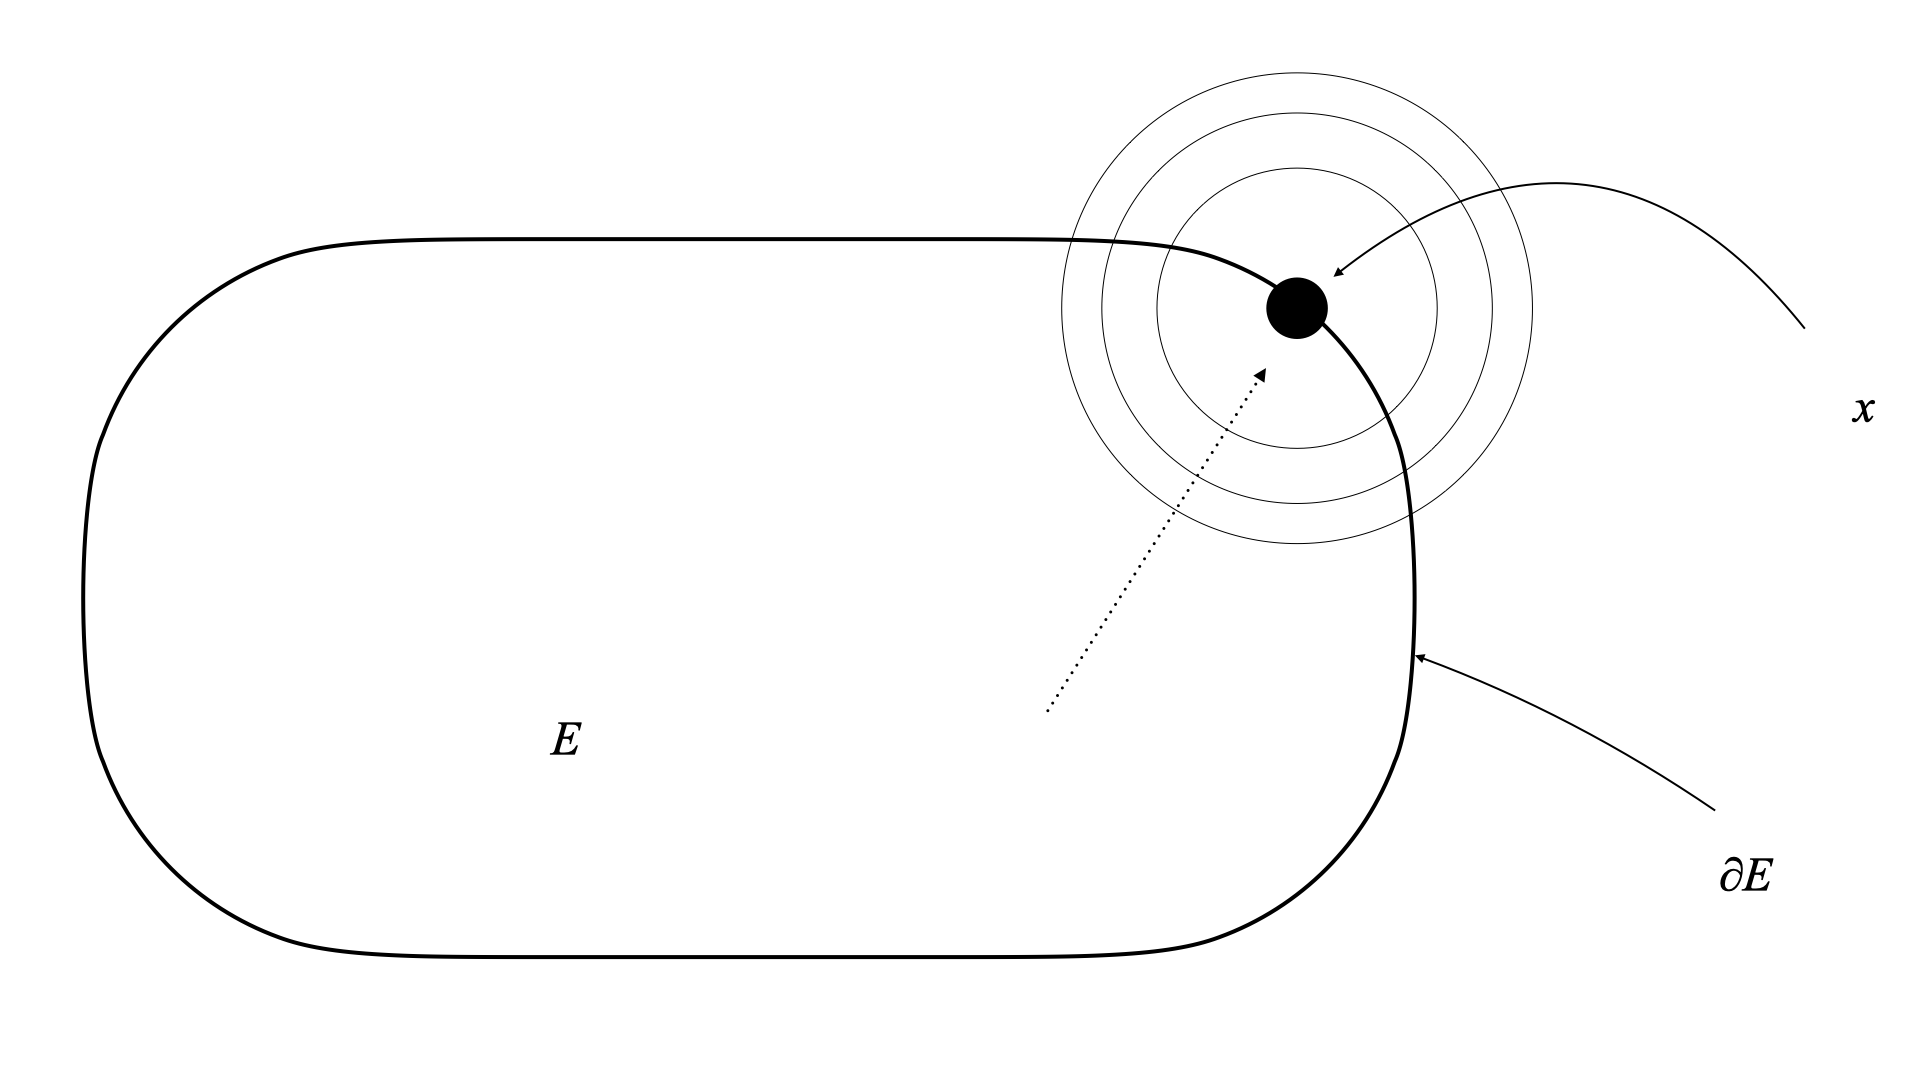
\includegraphics[width=6cm]{ch2_prob1_1.png}
    \caption{閉集合$E$と境界$\partial E$}
    \label{ch2_prob1_1}
\end{figure}%

($\Leftarrow$)
$\partial E\subset E$とする。$x$が$E$の任意の集積点であるとき、$x\in E$であることを示せばよい。ここで、$\C$の任意の点は$E$の内点か外点か境界の点であることに注意する。

もし$E$の集積点$x$が$E$の外点であるとすると、ある$r\in\R$に対して$B_r(x)\subset E^c$($E^c$は$E$の補集合を表す)であるから、$x$が$E$の集積点であることに反する。

よって、$E$の集積点$x$は$E$の内点か境界の点である。内点ならば$x\in E$は明らかである。境界の点ならば$\partial E\subset E$という仮定から、やはり$x\in E$である。(証明終)

\begin{mysimplebox}{問2}
    点集合の境界は閉集合であることを示せ。 
\end{mysimplebox}
\paragraph{証明}
$E$を点集合とし、$x$を$\partial E$の集積点とする。$x\in\partial E$であることを示せばよい。

$x$を$E$の内点とすると、ある$n\in\N$に対して、$B_{1/n}(x)\subset E$である。一方、$x$は$\partial E$の集積点であるから、ある$y\in\partial E$が存在して、$y\in B_{1/n}(x)\subset E$である。十分小さい$n'\in\N$をとれば、$B_{1/n'}(y)\subset E$であるから、$y$は$E$の内点である。しかし、これは$y\in\partial E$に反する。よって$x$は$E$の内点ではない。

$x$を$E$の外点としても同様の議論ができるから、$x$は$E$の外点でもない。

したがって、$x$は$E$の境界の点である。(証明終)

\begin{mysimplebox}{問3(Borel--Lebesgueの被覆定理)}
    有界な閉集合$E\subset\C$の各点においてそれぞれ1つの近傍が与えられているとする。
    そのとき、これら無数の近傍の中から有限個を選び出して、
    $E$のいかなる点もこれら有限個の近傍のいずれかに含まれるようにできる。
    これを示せ。
\end{mysimplebox}
\paragraph{証明}
有界な閉集合$E$の各点においてそれぞれ1つの近傍が与えられているとする。
このとき、$E$が有限被覆可能でないと仮定して矛盾を導く。

$E$が4点$R+Ri, -R+Ri, -R-Ri, R-Ri$を頂点とする閉正方形$Q_0$
に包まれるように正数$R$を大きくとる。$E$が有界であることから、これは可能である。

$Q_0$の対辺の中点を結んで$Q_0$を4つの閉正方形に分けると、
そのうちの少なくとも1つと$E$との共通部分は有限被覆可能でない。
その閉正方形を$Q_1$とする。

この手続きを繰り返して、閉正方形の列
$Q_0, Q_1, Q_2,\dots$を作る。
各$Q_k$と$E$の共通部分は、最初に与えられた$E$の各点の近傍に関して、
有限被覆可能ではない。

ここで、Weierstrass--Bolzanoの定理により、$\{Q_k\}$の部分列の中に
収束するものが存在する。
例えば閉正方形$Q_k$の右上の頂点を$a_k+b_{k}i (a_k,b_k\in\R)$、
左下の頂点を$c_k+d_{k}i (c_k,d_k\in\R)$とすると、
$\{a_k\}, \{b_k\},\{c_k\},\{d_k\}$にも収束する部分列がある。
$a_k-c_k=b_k-d_k=\frac{2R}{2^k}$であり、$k\longrightarrow\infty$の極限で0に収束するため、
区間縮小法により、$\{Q_k\}$の収束する部分列は1点に収束する。
$\{Q_k\}$の収束するある部分列を$\{Q'_k\}$とし、その収束点を$q$とする。

$\{Q'_k\}$の各項は$E$との共通部分が有限被覆可能でないから、
任意の$k$に対して$Q'_k\cap E\neq\emptyset$である。
よって、各$k$に対して$x_k\in Q'_k\cap E$をとることができる。
これは$q$の任意の近傍に$E$の点が存在することを示している。
ゆでに$q$は$E$の集積点である。
$E$が閉であることから$q\in E$である。

したがって、最初に$E$の各点に与えられた近傍として、
$q$にも近傍$V_q$が与えられており、
十分大きい$k$ に対して$Q'_k\subset V_q$である。

これは$Q'_k$が有限被覆可能でないことに反する。(証明終)

\begin{mysimplebox}{問4}
    $c$が定数のとき$|z-c|$は全平面で連続な函数であることを示せ。
\end{mysimplebox}
\paragraph{証明}
$f(z)=|z-c|$とする。
\begin{align*}
    f(z)-f(z')&=|z-c|-|z'-c|\\
    &\le |(z-c)-(z'-c)|\\
    &=|z-z'|
\end{align*}
よって、任意の$z\in\C$、任意の$\epsilon>0$に対して
$|z-z'|<\epsilon$となるように$z'\in\C$をとれば
$|f(z)-f(z')|<\epsilon$とできる。
ゆえに$f(z)$は全平面で連続である。(証明終)

\begin{mysimplebox}{問5}
    点$c$と閉集合$E$の距離が$d$ならば$d=|z-c|, z\in E$となる$z$が存在することを示せ。
\end{mysimplebox}
\paragraph{証明}
\begin{align*}
    d\coloneqq \inf_{z\in E}|z-c|
\end{align*}
である。

$d=|z-c|$となる$z\in E$が存在しないと仮定すると、
任意の$\epsilon>0$に対して$d<|z'-c|<d+\epsilon$となる$z'\in E$を
無数にとることができる。

\begin{align*}
    d+\epsilon>|z_1-c|>|z_2-c|>\dots>d
\end{align*}
となるように$E$の列$\{z_n\}$をとる。すべての$z_n$は$c$からの距離が
$d+\epsilon$以内に収まっている。すなわち有界である。

よって、列$\{z_n\}$は収束する部分列$\{z_{n_k}\}$を有する。
$z_{n_k}\longrightarrow c'$とする。$c'$は$E$の集積点であり、$E$は閉集合であるから$c'\in E$である。

仮定より$|c'-c|>d$であるから$|c'-c|>|z_{n_k}-c|>d$となる$z_{n_k}\in E$が存在する。しかし$z_{n_k}\longrightarrow c'$であり、
\begin{align*}
    |z_{n_k}-c|>|z_{n_{k+1}}-c|>\dots>|c'-c|.
\end{align*}
よって矛盾である。(証明終)

\begin{mysimplebox}{問6}
    $E, E'$がともに閉集合で、そのうちの1つが有界であるとき、$E$と$E'$の距離が$d$ならば$d=|z-z'|, z\in E, z'\in E'$となる$z, z'$が存在することを示せ。
\end{mysimplebox}
\paragraph{証明}
\begin{align*}
    d\coloneqq \inf_{z\in E, z'\in E'}|z-z'|
\end{align*}
である。

$E\cap E'\neq \emptyset$ならば、$d=0$であり、$z\in E\cap E'$
に対して$|z-z|=0=d$となり証明が終わる。

$E\cap E'=\emptyset$とする。$E$と$E'$の距離が$d$であるとする。
また、$E$は有界であるとする。
$d=|z-z'|$となる$z\in E, z'\in E'$が存在しないとすると、
\begin{align*}
    |z_1-z'_1|>|z_2-z'_2|>\dots>d
\end{align*}
となる列$\{z_k\}_{k=1,2,\dots}\subset E, \{z'_k\}_{k=1,2,\dots}\subset E'$が存在する。

$E$は有界であるから、$\{z_k\}$は収束する部分列を有する。
それを$\{z_{k_l}\}_{l=1,2,\dots}$とし、$z_{k_l}\longrightarrow c$とする。$c$は$E$の集積点であり$E$は閉集合であるから、$c\in E$である。

ここで$\{z_{k_l}\}_{l=1,2,\dots}$に対応する$\{z'_{k_l}\}_{l=1,2,\dots}$について考える。
任意の$\epsilon>0$に対して$l$を十分大きくとれば、
$d<|z_{k_l}-z'_{k_l}|<d+\epsilon/2$とできる。
また同時に$|c-z_{k_l}|<\epsilon/2$とできる。
よって$|c-z'_{k_l}|\le|c-z_{k_l}|+|z_{k_l}-z'_{k_l}|<\epsilon/2+\epsilon/2=\epsilon$である。
すなわち$\{z'_{k_l}\}_{l=1,2,\dots}$は有界であるから、収束する部分列を有する。
それを$\{z'_{k_{l_m}}\}_{m=1,2,\dots}$とし、$z'_{k_{l_m}}\rightarrow c'$とする。
$c'$は$E'$の集積点であり$E'$は閉集合であるから、$c'\in E'$である。

仮定より$|c'-c|>d$であるから$|c'-c|>|z_{k_{l_m}}-z'_{k_{l_m}}|>d$となる$m$が存在する。しかし$z_{k_{l_m}}\longrightarrow c$、$z'_{k_{l_m}}\longrightarrow c'$であり、
\begin{align*}
    |z_{k_{l_m}}-z'_{k_{l_m}}|>|c-c'|.
\end{align*}
よって矛盾である。(証明終)

\begin{mysimplebox}{問7}
    閉領域は連続体であることを示せ。
\end{mysimplebox}
\paragraph{証明}
$D$を領域(弧状連結である集合)とし、$\overline{D}\coloneqq D\cup\partial D$とする。
$\overline{D}$が連続体(連結)であることを背理法によって示す。

$\overline{D}=A_1\cup A_2$($A_1, A_2$はともに閉集合、$A_1\neq\emptyset, A_2\neq\emptyset$、$A_1\cap A_2=\emptyset$)とする。

$A_1\cap D\neq\emptyset$かつ$A_2\cap D\neq\emptyset$の場合、
$x_1\in A_1\cap D$、$x_2\in A_1\cap D$とすると、
$x_1$と$x_2$を結ぶ$D$内の曲線がある。それを、
\begin{align*}
    C\colon z=z(t)\quad (0\le t \le 1)
\end{align*}
とする。ただし$z(0)=x_1, z(1)=x_2$である。

曲線$C$上の点は$A_1$か$A_2$のどちらか一方に属する。
$z(t)\in A_1$である$t$の上限を$t_0$とすると、
$z(t_0)$の任意の近傍に$A_1$の点と$A_2$の点が存在する。
すなわち$z(t_0)$は$A_1$の集積点であり$A_2$の集積点でもある。
$A_1$、$A_2$はともに閉集合であるから$z(t_0)\in A_1\cap A_2$である。
これは$A_1\cap A_2=\emptyset$と矛盾する。

次に$A_1\cap D=\emptyset$または$A_2\cap D=\emptyset$の場合を考える。$A_1\cap D=\emptyset$かつ$A_2\cap D=\emptyset$となることはないから、$A_1\cap D=\emptyset$かつ$A_2\cap D\neq\emptyset$としてよい。このとき$A_1\subset\partial D$である。

$x_3\in A_1\subset\partial D$とする。$x_3$の任意の近傍に$D$の点が存在する。それらはすべて$A_2$の点である。よって$x_3$は$A_2$の集積点である。$A_2$は閉集合であるから$x_3\in A_2$となり、$A_1\cap A_2=\emptyset$と矛盾する。(証明終)

\begin{mysimplebox}{問8}
    $|\zeta|=1$のとき$\phi(\zeta)=\arg \zeta$とおくと、
    $|z|<1$で連続で境界$|\zeta|=1$の各点$\zeta$で境界値が$\phi(\zeta)$に等しいような函数は存在しないことを示せ。
\end{mysimplebox}
\paragraph{証明}
背理法によって証明する。
函数$f(z)$は$|z|<1$で連続で境界$|\zeta|=1$の各点$\zeta$で境界値が$\phi(\zeta)$に等しいとする。
このとき書籍p.32の事実により$f(z)$は境界$|\zeta|=1$においても連続である。
そこで$z=e^{i\theta}$とすると,
これは境界上の点であり$\theta=0$と$\theta=2\pi$は同じ点$z=1$を表す。$f(z)$の境界値は$\phi(z)$であるから
\begin{align*}
    \lim_{\theta\to 2\pi-0}f(e^{i\theta})
    &=\lim_{\theta\to 2\pi-0}\phi(e^{i\theta})\\
    &=\lim_{\theta\to 2\pi-0}\theta\\
    &=2\pi
\end{align*}
しかし$f(1)=\phi(1)=\arg 1=0\neq 2\pi$であるから$f(z)$が境界上で連続であることと矛盾する。よってこのような函数$f(z)$は存在しない。(証明終)

\begin{mysimplebox}{問9}
    \begin{align*}
        \sum_{n=1}^{\infty}\frac{z^2}{(1+|z|^2)^n}
    \end{align*}
    は$|z|<1$で収束するが広義の一様収束をしないことを示せ。
\end{mysimplebox}
\paragraph{証明}
\begin{align*}
    S=\sum_{n=1}^{\infty}\frac{z^2}{(1+|z|^2)^n}
\end{align*}
とおく。$z=0$のとき$S=0$である。

$z\neq 0$のとき、
\begin{align*}
    0<\frac{1}{1+|z|^2}<1.
\end{align*}
よって、
\begin{align*}
    S&=z^2\frac{1}{1+|z|^2}\frac{1}{1-\frac{1}{1+|z|^2}}\\
    &=z^2\frac{1}{1+|z|^2}\frac{1+|z|^2}{1+|z|^2-1}\\
    &=\frac{z^2}{|z|^2}
\end{align*}
$z=re^{i\theta} (r>0)$とすると$S=\frac{r^2e^{2i\theta}}{r^2}=e^{2i\theta}$である。すなわち
\begin{align*}
    S=\left\{
        \begin{array}{cc}
            0 & (z=0)\\
            e^{2i\theta} & (z\neq 0)
        \end{array}
    \right.
\end{align*}
よって$S$は$z=0$で連続でない。

書籍のp.35の事実「函数列が領域で連続かつ広義の一様収束をするならば極限函数も領域で連続である」ということから、もし$S$が広義の一様収束によって得られた極限函数ならば連続であるはずであるが、上で見たように不連続であるから、$S$は広義の一様収束による極限函数ではない。(証明終)

\begin{mysimplebox}{問10(Abelの連続定理)}
    $\sum_{n=0}^{\infty}c_nz^n$の収束半径が1に等しいとき、
    $\sum_{n=0}^{\infty}c_n$が収束すれば、
    \begin{align*}
        \lim_{x\to 1-0}\sum_{n=0}^{\infty}c_nx^n=\sum_{n=0}^{\infty}c_n
    \end{align*}
    であることを示せ。
\end{mysimplebox}
\paragraph{証明の前に}
$\lim_{x\to 1-0}$は実軸に沿っての極限である。
示すべきことは、整級数を収束円内から半径に沿って境界への極限をとれば、
境界値となることである。
極限操作と無限和の操作の順序を入れ替えてよいとも言える。
ただし、書籍のp.38に書かれてある「ヒント: 演習問題I-9」というのはよく分からなかった。
以下の解答は高木貞治『解析概論』に倣った。

\paragraph{証明}
\begin{align*}
    s_k\coloneqq\sum_{n=0}^{k}c_n
\end{align*}
とする。
$\sum_{n=0}^{\infty}c_n$が収束するから、任意の$\delta>0$に対して
十分大きい$n$をとれば、$l>m>n$に対して
\begin{align*}
    |s_l-s_m|<\delta
\end{align*}
とできる。

$m>n$となるある$m$を固定し、$k>m$のとき$\sigma_k\coloneqq s_k-s_m$とおくと$|\sigma_l|<\delta$である。

$0\le x\le 1$とすれば、$x^n\le x^{n+1}$から
\begin{align*}
    \left|\sum_{n=m+1}^{l}c_nx^n\right|
    &=\left|(s_{m+1}-s_m)x^{m+1}+(s_{m+2}-s_{m+1})x^{m+2}+\dots+(s_l-s_{l-1})x^l\right|\\
    &=\left|\sigma_{m+1}x^{m+1}+(\sigma_{m+2}-\sigma_{m+1})x^{m+2}+\dots+(\sigma_l-\sigma_{l-1})x^l\right|\\
    &=\left|\sigma_{m+1}(x^{m+1}-x^{m+2})+\sigma_{m+2}(x^{m+2}-x^{m+3})+\dots+\sigma_{l-1}(x^{l-1}-x^l)+\sigma_lx^l\right|\\
    &\le\delta\left|(x^{m+1}-x^{m+2})+(x^{m+2}-x^{m+3})+\dots+(x^{l-1}-x^l)+x^l\right|\\
    &=\delta x^{m+1}\le\delta
\end{align*}
ゆえに$\sum_{n=0}^{\infty}c_nz^n$は$0\le x\le 1$において一様収束する。書籍p.35の事実により、極限函数は$0\le x\le 1$において連続である。

したがって
\begin{align*}
    \lim_{x\to 1-0}\sum_{n=0}^{\infty}c_nx^n=\sum_{n=0}^{\infty}c_n
\end{align*}
(証明終)
\chapter{導函数}%第3章

\begin{mysimplebox}{問1}
    Cauchy--Riemannの関係式は次の関係式と同等であることを示せ:
    \begin{align*}
        \frac{\partial P}{\partial r}
        =\frac{1}{r}\frac{\partial Q}{\partial \theta},\quad
        \frac{\partial P}{\partial \theta}
        =-r\frac{\partial Q}{\partial r}\quad
        (z=re^{\theta i},r\neq0)
    \end{align*}
\end{mysimplebox}
\paragraph{証明}
$z=re^{\theta i}=r(\cos\theta+i\sin\theta)$、
$x=r\cos\theta,y=r\sin\theta$である。

$x^2+y^2=r^2, \frac{y}{x}=\tan\theta$より
\begin{align*}
    &\frac{\partial r}{\partial x}=\frac{x}{r}=\cos\theta,\quad
    \frac{\partial \theta}{\partial x}=-\frac{\sin\theta}{r}\\
    &\frac{\partial r}{\partial y}=\frac{y}{r}=\sin\theta,\quad
    \frac{\partial \theta}{\partial y}=\frac{\cos\theta}{r}
\end{align*}
である。

微分の変数変換によって以下のような計算ができる。
\begin{align*}
    \begin{bmatrix}
        P_x & Q_x\\
        P_y & Q_y
    \end{bmatrix}
    &=
    \begin{bmatrix}
        \frac{\partial r}{\partial x} & \frac{\partial \theta}{\partial x}\\
        \frac{\partial r}{\partial y} & \frac{\partial \theta}{\partial y}
    \end{bmatrix}
    \begin{bmatrix}
        P_r & Q_r\\
        P_\theta & Q_\theta
    \end{bmatrix}
    =
    \begin{bmatrix}
        \cos\theta & -\frac{\sin\theta}{r}\\
        \sin\theta & \frac{\cos\theta}{r}
    \end{bmatrix}
    \begin{bmatrix}
        P_r & Q_r\\
        P_\theta & Q_\theta
    \end{bmatrix}\\
    %%%%%%%%%%%%%%%%%%%%%
    \begin{bmatrix}
        P_r & Q_r\\
        P_\theta & Q_\theta
    \end{bmatrix}
    &=
    \begin{bmatrix}
        \cos\theta & -\frac{\sin\theta}{r}\\
        \sin\theta & \frac{\cos\theta}{r}
    \end{bmatrix}^{-1}
    \begin{bmatrix}
        P_x & Q_x\\
        P_y & Q_y
    \end{bmatrix}
    =
    \begin{bmatrix}
        \cos\theta & \sin\theta\\
        -r\sin\theta & r\cos\theta
    \end{bmatrix}
    \begin{bmatrix}
        P_x & Q_x\\
        P_y & Q_y
    \end{bmatrix}
\end{align*}
Cauchy--Riemannの関係式より,
$P_x=Q_y, P_y=-Q_x$であるから
\begin{align*}
    \begin{bmatrix}
        P_r & Q_r\\
        P_\theta & Q_\theta
    \end{bmatrix}
    =
    \begin{bmatrix}
        \cos\theta & \sin\theta\\
        -r\sin\theta & r\cos\theta
    \end{bmatrix}
    \begin{bmatrix}
        P_x & -P_y\\
        P_y & P_x
    \end{bmatrix}
\end{align*}

$P_x=P_y=0$のとき$P_r=P_\theta=Q_r=Q_\theta=0$であるから示すべき式が成り立つ\footnote{上の行列の式よりすぐに極座標でのCauchy--Riemannの関係式が導かれるが、ここではわざわざ回転行列で書いた。}。

$P_x^2+P_y^2\neq0$であるとき、
$\frac{P_x}{\sqrt{P_x^2+P_y^2}}=\cos\alpha,
\frac{P_y}{\sqrt{P_x^2+P_y^2}}=\sin\alpha$とする。
$R(\theta)=
\begin{bmatrix}
    \cos\theta & -\sin\theta\\
    \sin\theta & \cos\theta
\end{bmatrix}$とすると
\begin{align*}
    \begin{bmatrix}
        P_r & Q_r\\
        P_\theta & Q_\theta
    \end{bmatrix}
    &=
    \begin{bmatrix}
        1 & 0\\
        0 & r
    \end{bmatrix}
    R(-\theta)\cdot\sqrt{P_x^2+P_y^2}R(\alpha)
    =\sqrt{P_x^2+P_y^2}
    \begin{bmatrix}
        1 & 0\\
        0 & r
    \end{bmatrix}
    R(\alpha-\theta)
\end{align*}

よって、
\begin{align*}
    P_r&=\frac{1}{r}Q_\theta=\sqrt{P_x^2+P_y^2}\cos(\alpha-\theta)\\
    P_\theta&=-rQ_r=-\sqrt{P_x^2+P_y^2}\sin(\alpha-\theta)
\end{align*}

逆に、$P_r=\frac{1}{r}Q_\theta,P_\theta=-rQ_r$が成り立つとき
\begin{align*}
    \begin{bmatrix}
        P_x & Q_x\\
        P_y & Q_y
    \end{bmatrix}
    &=
    \begin{bmatrix}
        \cos\theta & -\frac{\sin\theta}{r}\\
        \sin\theta & \frac{\cos\theta}{r}
    \end{bmatrix}
    \begin{bmatrix}
        P_r & Q_r\\
        P_\theta & Q_\theta
    \end{bmatrix}
    =
   R(\theta)
    \begin{bmatrix}
        1 & 0\\
        0 & \frac{1}{r}
    \end{bmatrix}
    \begin{bmatrix}
        P_r & Q_r\\
        P_\theta & Q_\theta
    \end{bmatrix}\\
    &=
    R(\theta)
    \begin{bmatrix}
        P_r & Q_r\\
        \frac{1}{r}P_\theta & \frac{1}{r}Q_\theta
    \end{bmatrix}
    =
    R(\theta)
    \begin{bmatrix}
        P_r & Q_r\\
        -Q_r & P_r
    \end{bmatrix}
\end{align*}
これより$P_x=Q_y,P_y=-Q_x$が成り立つ。(証明終)

\begin{mysimplebox}{問2}
領域$|z|>0$、$|\arg z|<\pi$で$h(z)=\log|z|+i\arg z$は正則で、
$z=e^{h(z)}=\exp(\log|z|+i\arg z)$であることを示せ。
\end{mysimplebox}
\paragraph{証明}
$r=|z|$、$\theta=\arg z$であるから$h(z)=\log r+i\theta$である。
ただし、$-\pi<\theta<\pi$である。

$P(r,\theta)=\log r, Q(r,\theta)=\theta$とすると
\begin{align*}
    &P_r=\frac{1}{r},\quad
    Q_r=0\\
    &P_\theta=0,\quad
    Q_\theta=1
\end{align*}
である。
よって、$P_r=\frac{1}{r}Q_\theta,P_\theta=-rQ_r$が満たされるため、問1により$h(z)$は$r>0,|\theta|<\pi$で正則である。

また
\begin{align*}
    e^{h(z)}&=e^{\log r+i\theta}=e^{\log r}e^{i\theta}\\
    &=r(\cos\theta+i\sin\theta)=x+iy=z
\end{align*}
(証明終)

\begin{mysimplebox}{問3}
    $c\neq0,e^z=c$である$z$のなかには不等式$|z|\le|\log|c||+\pi$を満たすものが必ず存在することを示せ。
\end{mysimplebox}
\paragraph{証明}
複素平面上の$c\neq0$は$c=|c|e^{i\theta}\ (-\pi\le\theta<\pi)$と書くことができる。

$z=\log|c|+i\theta$とすると
\begin{align*}
    e^z&=e^{\log|c|+i\theta}=e^{\log|c|}e^{i\theta}\\
    &=|c|(\cos\theta+i\sin\theta)=c
\end{align*}
である。

この$z$は次を満たす。
\begin{align*}
    |z|&=|\log|c|+i\theta|\le|\log|c||+|\theta|\le|\log|c||+\pi
\end{align*}
(証明終)

\begin{mysimplebox}{問4}
    $z=c$で$f(z)$が微分可能ならば、
    $z=\overline{c}$で$\overline{f(\overline{z})}$
    は微分可能であることを示せ。
    ただし、$\Im c\neq0$である。
\end{mysimplebox}
\paragraph{証明}
次の極限値が存在するとする。
\begin{align*}
    \lim_{z\to c}\frac{f(z)-f(c)}{z-c}=f'(c)
\end{align*}    
%$\lim_{z\to c}\frac{f(z)-f(c)}{z-c}$は存在するとする。
このとき
\begin{align*}
    \lim_{z\to\overline{c}}
    \frac{\overline{f(\overline{z})}-\overline{f(\overline{\overline{c}})}}{z-\overline{c}}
    &=\lim_{z\to\overline{c}}
    \frac{\overline{f(\overline{z})}-\overline{f(c)}}{z-\overline{c}}
    =\lim_{w\to c}
    \frac{\overline{f(w)}-\overline{f(c)}}{\overline{w}-\overline{c}}
    =\overline{\lim_{w\to c}\frac{f(w)-f(c)}{w-c}}
    =\overline{f'(c)}
\end{align*}
である。ただし、途中で$w=\overline{z}$とおいた。
これで$z=\overline{c}$で$\overline{f(\overline{z})}$は微分可能であることを示せたうえに、その微分係数が$\overline{f'(c)}$であることもわかった。(証明終)

\begin{mysimplebox}{問5}
    $\overline{z}$を$z$の有理函数として表すことは不可能であることを示せ。
\end{mysimplebox}
\paragraph{証明}
$z=x+iy\ (x,y\in\R)$とする。

実函数$P(x,y),Q(x,y)$によって$\overline{z}=P(x,y)+iQ(x,y)$とすると
\begin{align*}
    P(x,y)=x,\quad Q(x,y)=-y
\end{align*}
である。
\begin{align*}
    &P_x=1,\quad Q_x=0\\
    &P_y=0,\quad Q_y=-1
\end{align*}
であるから、$\overline{z}$はCauchy--Riemannの関係式を満たさない。
ゆえに$\overline{z}$は正則でない。

ここで
\begin{align*}
    \overline{z}=\frac{a_0+a_1z+\cdots+a_nz^n}{b_0+b_1z+\cdots+b_mz^m}
\end{align*}
と書けるとする。
この右辺は分母の零点を除いた領域で正則である。
しかし左辺は正則でないから矛盾である。
よって、$\overline{z}$を$z$の有理函数として表すことは不可能である。(証明終)

\begin{mysimplebox}{問6}
    $f(z)$は領域$D$で正則な函数、$C$は$D$の2点$c_1, c_2$を結ぶ$D$内の線分であるとき、$C$上の2点$c, c'$を適当に選べば
    \begin{align*}
        f(c_2)-f(c_1)=(c_2-c_1)[\Re (f'(c))+i\Im(f'(c'))]
    \end{align*}
    とできることを示せ。
\end{mysimplebox}
\paragraph{証明}
$f(z)$の実部と虚部を$P(x,y),Q(x,y)$とする。
つまり、$z=x+yi$($x,y\in\R$)に対して実数関数$P(x,y),Q(x,y)$によって$f(z)=P(x,y)+iQ(x,y)$と書けるとする。
さらに
\begin{align*}
    c_1&=a+bi\\
    c_2&=a+h+(b+k)i
\end{align*}
とする。
ただし、$a,b,h,k\in\R$である。

線分$C$上の点は$t\in[0,1]$によって、
\begin{align*}
    c_1+t(c_2-c_1)=a+bi+t(h+ki)=a+th+(b+tk)i
\end{align*}
と表される。

ここで、次のように$t$に関する函数$g(t)$を定義する。
\begin{align*}
    g(t)&=\frac{f(c_1+t(c_2-c_1))}{c_2-c_1}\\
    &=\frac{P(a+th,b+tk)+iQ(a+th,b+tk)}{h+ki}\\
    &=\frac{(P+iQ)(h-ki)}{h^2+k^2}=\frac{Ph+Qk+i(Qh-Pk)}{h^2+k^2}
\end{align*}

$g(t)$の実部と虚部を$U(t),V(t)$とする。次が成り立つ。
\begin{align*}
    U(t)&=\frac{P(a+th,b+tk)h+Q(a+th,b+tk)k}{h^2+k^2}\\
    V(t)&=\frac{Q(a+th,b+tk)h-P(a+th,b+tk)k}{h^2+k^2}
\end{align*}

$U(t),V(t)$は$t$に関する連続函数であるから、平均値の定理により次が成り立つ。
\begin{align*}
    g(1)-g(0)&=\frac{f(c_2)-f(c_1)}{c_2-c_1}=U(1)-U(0)+i(V(1)-V(0))\\
    &=U'(\theta_1)+iV'(\theta_2)
\end{align*}
ただし、$\theta_1,\theta_2\in(0,1)$である。

Cauchy--Riemannの関係式から、次が成り立つ。
\begin{align*}
    U'(t)=\frac{1}{h^2+k^2}
    &\left\{P_x(a+th,b+tk)h^2+P_y(a+th,b+tk)hk\right.\\
    &\left.+Q_x(a+th,b+tk)hk+Q_y(a+th,b+tk)k^2\right\}\\
    =\frac{1}{h^2+k^2}
    &\left\{P_x(a+th,b+tk)h^2
    +Q_y(a+th,b+tk)k^2\right\}\\
    =\frac{1}{h^2+k^2}
    &P_x(a+th,b+tk)(h^2+k^2)=P_x(a+th,b+tk)\\
    %%%%%%
    V'(t)=\frac{1}{h^2+k^2}
    &\left\{Q_x(a+th,b+tk)h^2+Q_y(a+th,b+tk)hk\right.\\
    &\left.-P_x(a+th,b+tk)hk-P_y(a+th,b+tk)k^2\right\}\\
    =\frac{1}{h^2+k^2}
    &\left\{Q_x(a+th,b+tk)h^2
    -P_y(a+th,b+tk)k^2\right\}\\
    =\frac{1}{h^2+k^2}
    &Q_x(a+th,b+tk)(h^2+k^2)=Q_x(a+th,b+tk)
\end{align*}

よって、
\begin{align*}
    c&=c_1+\theta_1(c_2-c_1)=a+\theta_1 h+(b+\theta_1 k)i\\
    c'&=c_1+\theta_2(c_2-c_1)=a+\theta_2 h+(b+\theta_2 k)i
\end{align*}
とすると、
\begin{align*}
    \frac{f(c_2)-f(c_1)}{c_2-c_1}
    &=P_x(a+\theta_1 h,b+\theta_1 k)+iQ_x(a+\theta_2 h,b+\theta_2 k)\\
    &=\Re(f'(c))+i\Im(f'(c'))
\end{align*}
ここで$f'(z)=P_x+iQ_x$であることを用いた。

以上より、
\begin{align*}
    f(c_2)-f(c_1)=(c_2-c_1)[\Re(f'(c))+i\Im(f'(c'))]
\end{align*}
が成り立つ。
(証明終)
\chapter{積分}%第4章

\begin{mysimplebox}{問1}
   $\int_{0}^{1+i}\Re(z)dz$($z=0$から$z=1+i$に至る線分に沿って)
\end{mysimplebox}
\paragraph{解}
この積分路では$z=x+ix$であり、$x$は0から1まで動くから
\begin{align*}
    \int_{0}^{1+i}\Re(z)dz
    &=\int_{0}^{1}xd(x+ix)
    =\int_{0}^{1}x(1+i)dx
    =(1+i)\left[\frac{x^2}{2}\right]_0^1
    =\frac{1+i}{2}
\end{align*}

\begin{mysimplebox}{問2}
    $\int_{-i}^{i}|z|dz$(円$|z|=1$の左半分に沿って)
 \end{mysimplebox}
 \paragraph{解}
 \begin{align*}
    \int_{-i}^{i}|z|dz
    &=\int_{\frac{3\pi}{2}}^{\frac{\pi}{2}}|e^{i\theta}|d(e^{i\theta})
    =\int_{\frac{3\pi}{2}}^{\frac{\pi}{2}}ie^{i\theta}d\theta
    =\left[e^{i\theta}\right]_{\frac{3\pi}{2}}^{\frac{\pi}{2}}
    =e^{\frac{\pi}{2}}-e^{\frac{3\pi}{2}}=i-(-i)=2i
\end{align*}

\begin{mysimplebox}{問3}
   $\int_{|z|=1}|z-1||dz|$(正の向き)
\end{mysimplebox}
\paragraph{解}
\begin{align*}
   \int_{|z|=1}|z-1||dz|
   &=\int_{0}^{2\pi}|e^{i\theta}-1||d(e^{i\theta})|
   =\int_{0}^{2\pi}|\cos \theta-1+i\sin \theta||ie^{i\theta}d\theta|\\
   &=\int_{0}^{2\pi}\sqrt{(\cos\theta-1)^2+\sin^2\theta}d\theta
   =\int_{0}^{2\pi}\sqrt{2(1-\cos\theta)}d\theta\\
   &=2\int_{0}^{2\pi}\sqrt{\sin^2\frac{\theta}{2}}d\theta
   =2\int_{0}^{2\pi}\left|\sin\frac{\theta}{2}\right|d\theta\\
   &=2\int_{0}^{2\pi}\sin\frac{\theta}{2}d\theta
   =2\left[-2\cos\frac{\theta}{2}\right]_0^{2\pi}\\
   &=-4(-1-1)=8
\end{align*}

\begin{mysimplebox}{問4}
   $\int_{|z|=1}\frac{e^z}{z^2}dz$(正の向き)
\end{mysimplebox}
\paragraph{解}
\begin{align*}
   \int_{|z|=1}\frac{e^z}{z^2}dz
   &=\int_{|z|=1}\frac{1}{z^2}\left(1+z+\frac{1}{2!}z^2+\dots\right)dz
   =\int_{|z|=1}\frac{1}{z}dz=2\pi i
\end{align*}

\begin{figure}[h]
   \centering
   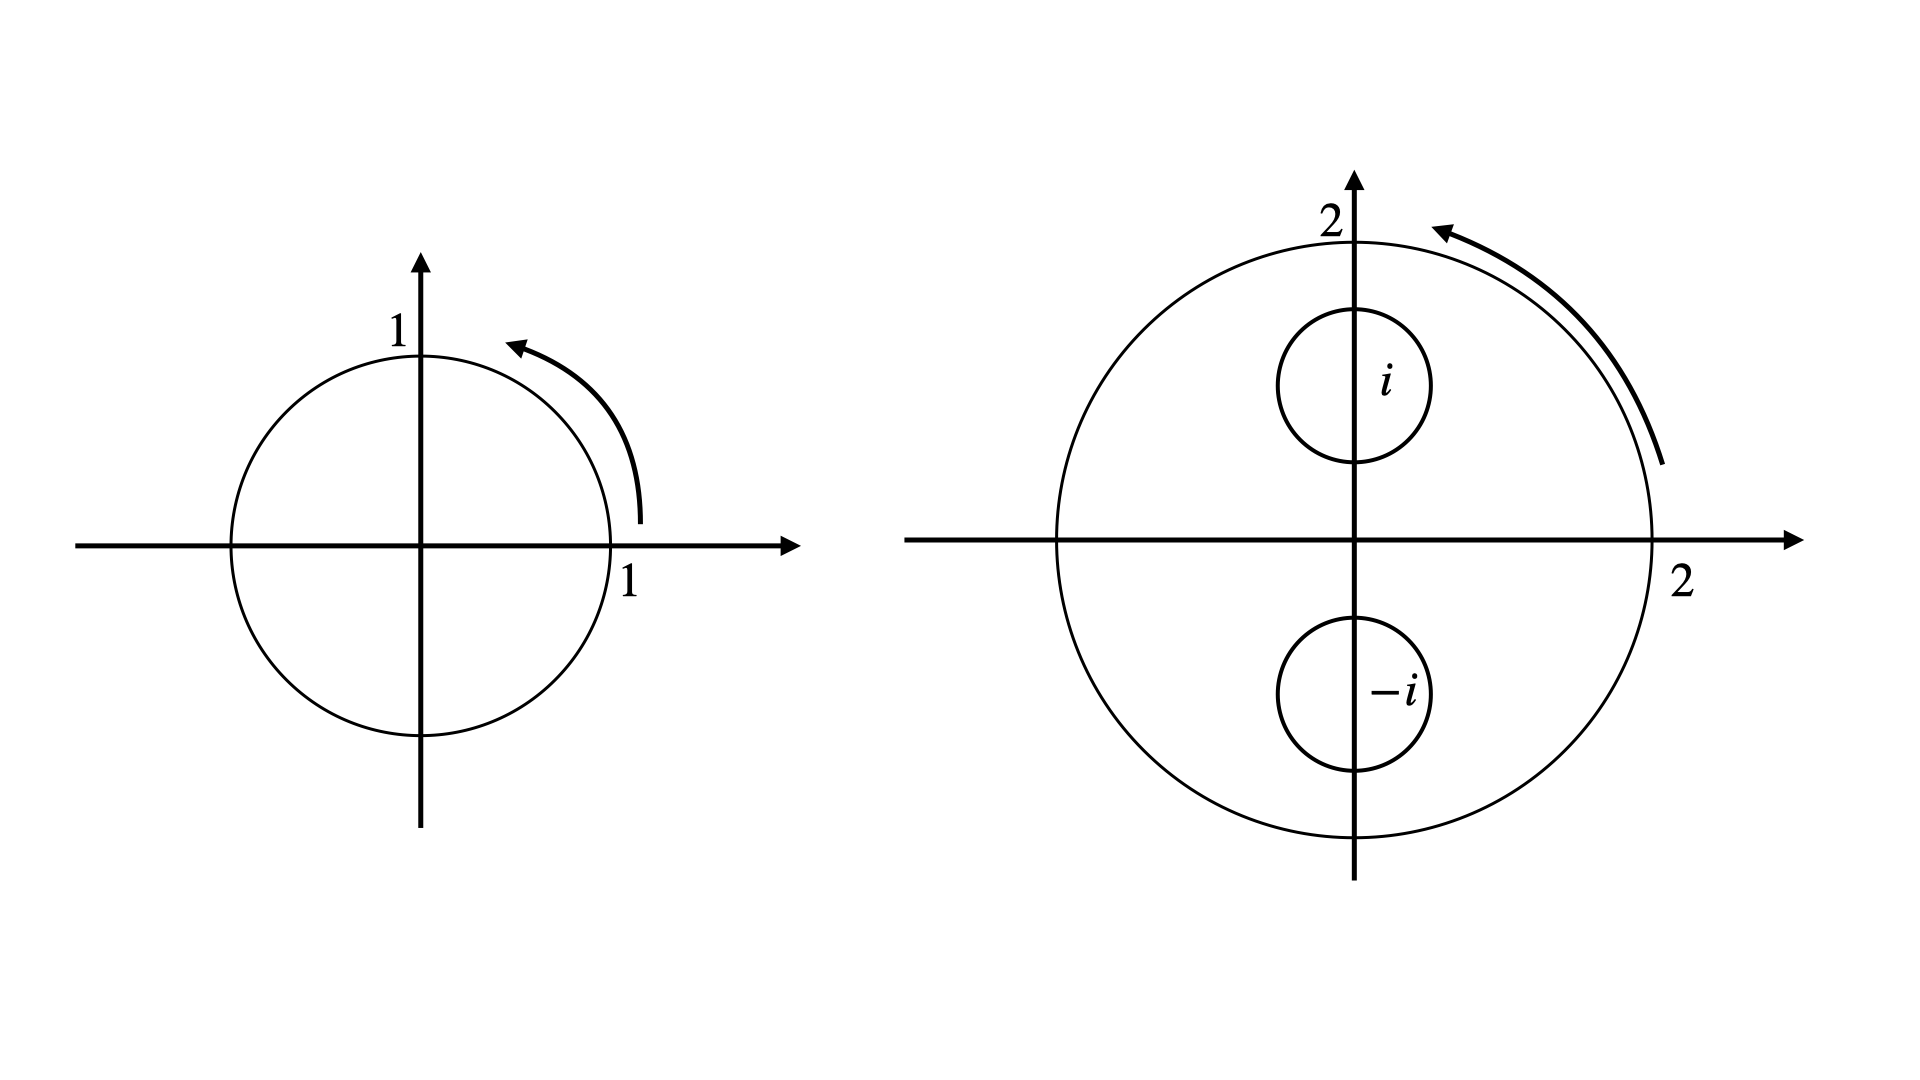
\includegraphics[width=10cm]{chap4_fig/chap4_fig001.png}
   \caption{積分路}
   \label{fig:chap4}
\end{figure}

\begin{mysimplebox}{問5}
   $\int_{|z|=2}\frac{dz}{1+z^2}$(正の向き)
\end{mysimplebox}
\paragraph{解}
\begin{align*}
   \int_{|z|=2}\frac{dz}{1+z^2}
   &=\int_{|z|=2}\frac{1}{2i}\left(\frac{1}{z-i}-\frac{1}{z+i}\right)dz
   =\frac{1}{2i}\left(\int_{|z|=2}\frac{dz}{z-i}-\int_{|z|=2}\frac{dz}{z+i}\right)\\
   &=\frac{1}{2i}(2\pi i-2\pi i)=0
\end{align*}

\begin{mysimplebox}{問6}
   $f(z)=\sum_{n=0}^{\infty}c_nz^n$の収束半径が$R(>0)$のとき
   \begin{align*}
      f(0)=\lim_{n\to\infty}\sum_{\nu=0}^{n}f(r\omega_n^\nu)\cdot n^{-1}\quad\left(0<r<R, \omega_n=\exp\left(\frac{2\pi i}{n}\right)\right)
   \end{align*}
   を示せ。
\end{mysimplebox}
\paragraph{証明}
$|r\omega_n^\nu|<R$であるから、$f(r\omega_n^\nu)$は収束する。

級数を次のように積分に変形できる。
\begin{align*}
   \frac{1}{n}\sum_{\nu=0}^{n}f(r\omega_n^\nu)
   &=\frac{1}{n}\sum_{\nu=0}^{n}f\left(r\exp\left(\frac{2\pi i\nu}{n}\right)\right)
   \overset{n\longrightarrow\infty}{\longrightarrow}
   \int_{0}^{1}f(r\exp(2\pi it))dt
\end{align*}

$f(z)$はべき級数であるから、項別積分可能である。
よって、
\begin{align*}
   \int_{0}^{1}f(r\exp(2\pi it))dt
   &=\int_{0}^{1}\sum_{n=0}^{\infty}c_nr^n\exp(2\pi int)dt
   =\sum_{n=0}^{\infty}c_nr^n\int_{0}^{1}\exp(2\pi int)dt\\
   &=c_0\int_{0}^{1}dt+\sum_{n=1}^{\infty}c_nr^n\int_{0}^{1}\exp(2\pi int)dt\\
   &=c_0+\sum_{n=1}^{\infty}c_nr^n\left[\frac{\exp(2\pi int)}{2\pi in}\right]_0^1\\
   &=c_0+\sum_{n=1}^{\infty}c_nr^n\frac{1}{2\pi in}\left\{\exp(2\pi in)-\exp(0)\right\}\\
   &=c_0=f(0)
\end{align*}
(証明終)

\begin{mysimplebox}{問7}
   \begin{align*}
      \int_{|z|=1}\left(z+\frac{1}{z}\right)^{2n}\frac{dz}{z}
   \end{align*}
   を求めることにより、
   \begin{align*}
      \int_{0}^{2\pi}\cos^{2n}\theta d\theta
      =2\pi\cdot\frac{1\cdot3\cdot5\cdot\dots\cdot(2n-1)}{2\cdot4\cdot6\cdot\dots\cdot2n}
   \end{align*}
   を示せ。
\end{mysimplebox}
\paragraph{証明}
$|z|=1$において$z=e^{i\theta}$であるから
\begin{align*}
   \int_{|z|=1}\left(z+\frac{1}{z}\right)^{2n}\frac{dz}{z}
   &=\int_{0}^{2\pi}\left(e^{i\theta}+\frac{1}{e^{i\theta}}\right)^{2n}\frac{de^{i\theta}}{e^{i\theta}}
   =\int_{0}^{2\pi}2^{2n}\cos^{2n}\theta\frac{ie^{i\theta}d\theta}{e^{i\theta}}\\
   &=2^{2n}i\int_{0}^{2\pi}\cos^{2n}\theta d\theta
\end{align*}

また、被積分函数を2項定理によって展開すると
\begin{align*}
   \int_{|z|=1}\left(z+\frac{1}{z}\right)^{2n}\frac{dz}{z}
   &=\int_{|z|=1}\sum_{k=0}^{2n}\binom{2n}{k}z^kz^{-(2n-k)}z^{-1}dz
   =\sum_{k=0}^{2n}\binom{2n}{k}\int_{|z|=1}z^{2k-2n-1}dz\\
   &=\binom{2n}{n}\int_{|z|=1}\frac{dz}{z}=2\pi i\binom{2n}{n}
\end{align*}

よって
\begin{align*}
   \int_{0}^{2\pi}\cos^{2n}\theta d\theta
   &=\frac{1}{2^{2n}i}2\pi i\binom{2n}{n}
   =2\pi\frac{1}{2^{2n}}\frac{(2n)!}{n!n!}\\
   &=2\pi\frac{(2n)!}{(2\cdot4\cdot6\cdots2n)^2}
   =2\pi\frac{1\cdot3\cdot5\dots(2n-1)}{2\cdot4\cdot6\cdots2n}
\end{align*}
(証明終)
\chapter{正則函数}%第5章

\begin{mysimplebox}{問1}
   $f(z)=u(r,\theta)+iv(r,\theta)$($z=re^{\theta i}$)が$|z|<R$で正則ならば
   \begin{align*}
    \frac{f^{(n)}(0)}{n!}
    =\frac{1}{\pi r^n}\int_{0}^{2\pi}u(r,\theta)e^{-in\theta}d\theta\quad(0<r<R)
   \end{align*}
\end{mysimplebox}
\paragraph{証明1}(泥臭い方法)
書籍のp.87の§28より、原点を中心とする半径$R$の円の内部において$f(z)$はべき級数で表される。
すなわち
\begin{align*}
    f(z)=c_0+c_1z+c_2+\dots+c_kz^k+\dots
    =\sum_{k=0}^{\infty}c_kz^k
\end{align*}
$\frac{f^{(n)}(0)}{n!}=c_n$である。

ここで$c_k=a_k+ib_k$($a_k,b_k\in\R$)とし、$f(z)$に$z=re^{\theta i}$を代入すると
\begin{align*}
    f(re^{\theta i})
    &=\sum_{k=0}^{\infty}(a_k+ib_k)r^ke^{k\theta i}\\
    &=\sum_{k=0}^{\infty}r^k(a_k+ib_k)(\cos k\theta+i\sin k\theta)\\
    &=\sum_{k=0}^{\infty}r^k\{a_k\cos k\theta-b_k\sin k\theta+i(a_k\sin k\theta+b_k\cos k\theta)\}
\end{align*}
$f(z)=u(r,\theta)+iv(r,\theta)$であるから
\begin{align*}
    u(r,\theta)
    =\sum_{k=0}^{\infty}r^k(a_k\cos k\theta-b_k\sin k\theta)
\end{align*}
$n=0$のときは$\int_{0}^{2\pi}u(r,\theta)d\theta=a_0\int_{0}^{2\pi}d\theta=2\pi a_0\neq \pi c_0$であり、成り立たない。よって$n\neq0$とする。

\begin{align*}
    u(r,\theta)e^{-in\theta}
    =&\sum_{k=0}^{\infty}r^k(a_k\cos k\theta-b_k\sin k\theta)(\cos n\theta-i\sin n\theta)\\
    =&\sum_{k=0}^{\infty}r^k
    \{a_k\cos k\theta\cos n\theta-b_k\sin k\theta\cos n\theta
    \\
    &-i(a_k\cos k\theta\sin n\theta-b_k\sin k\theta\sin n\theta)\}
\end{align*}
$k\neq n$のとき
\begin{align*}
    %%%cos cos
    \int_{0}^{2\pi}\cos k\theta\cos n\theta d\theta
    &=\int_{0}^{2\pi}\frac{1}{2}\{\cos(k+n)\theta+\cos(k-n)\theta\} d\theta\\
    &=\frac{1}{2}\left[\frac{\sin(k+n)\theta}{k+n}+\frac{\sin(k-n)\theta}{k-n}\right]_0^{2\pi}=0\\
    %%%sin cos
    \int_{0}^{2\pi}\sin k\theta\cos n\theta d\theta
    &=\int_{0}^{2\pi}\frac{1}{2}\{\sin(k+n)\theta+\sin(k-n)\theta\} d\theta\\
    &=-\frac{1}{2}\left[\frac{\cos(k+n)\theta}{k+n}+\frac{\cos(k-n)\theta}{k-n}\right]_0^{2\pi}=0\\
    %%%sin sin
    \int_{0}^{2\pi}\sin k\theta\sin n\theta d\theta
    &=\int_{0}^{2\pi}\frac{1}{2}\{\cos(k+n)\theta-\cos(k-n)\theta\} d\theta\\
    &=\frac{1}{2}\left[\frac{\sin(k+n)\theta}{k+n}+\frac{\sin(k-n)\theta}{k-n}\right]_0^{2\pi}=0
\end{align*}
一方、$k=n\neq0$のとき
\begin{align*}
    %%%cos cos
    \int_{0}^{2\pi}\cos n\theta\cos n\theta d\theta
    &=\int_{0}^{2\pi}\frac{1}{2}(\cos 2n\theta+1) d\theta\\
    &=\frac{1}{2}\left[\frac{\sin 2n\theta}{2n}+\theta\right]_0^{2\pi}=\pi\\
    %%%sin cos
    \int_{0}^{2\pi}\sin n\theta\cos n\theta d\theta
    &=\int_{0}^{2\pi}\frac{1}{2}\sin 2n\theta d\theta\\
    &=-\frac{1}{2}\left[\frac{\cos 2n\theta}{2n}\right]_0^{2\pi}=0\\
    %%%sin sin
    \int_{0}^{2\pi}\sin n\theta\sin n\theta d\theta
    &=\int_{0}^{2\pi}\frac{1}{2}\{1-\cos 2n\theta\} d\theta\\
    &=\frac{1}{2}\left[\theta-\frac{\sin 2n\theta}{2n}\right]_0^{2\pi}=\pi
\end{align*}
したがって
\begin{align*}
    \int_{0}^{2\pi}u(r,\theta)e^{-in\theta}d\theta
    &=r^n(\pi a_n+i\pi b_n)=\pi r^nc_n\\
    \frac{1}{\pi r^n}\int_{0}^{2\pi}u(r,\theta)e^{-in\theta}d\theta
    &=c_n
\end{align*}
これで$n\neq0$のときは示せた。
\paragraph{補足}
\begin{align*}
    \int_{0}^{2\pi}f(re^{\theta i})e^{-in\theta}d\theta
    &=\int_{0}^{2\pi}u(r,\theta)e^{-in\theta}d\theta
    +i\int_{0}^{2\pi}v(r,\theta)e^{-in\theta}d\theta\\
    &=2\pi c_nr^n
\end{align*}
よって、$n\neq0$に対して
\begin{align*}
    i\int_{0}^{2\pi}v(r,\theta)e^{-in\theta}d\theta
    &=\pi c_nr^n
\end{align*}
また、$n=0$のとき
\begin{align*}
    i\int_{0}^{2\pi}v(r,\theta)d\theta
    &=2\pi ib_0
\end{align*}

\paragraph{証明2}
$u(r,\theta)=\frac{1}{2}\{f(z)+\overline{f(z)}\}$であるから、$n\ge1$のとき、
\begin{align*}
    \frac{1}{\pi r^n}\int_{0}^{2\pi}u(r,\theta)e^{-in\theta}d\theta
    =\frac{1}{2\pi r^n}\int_{0}^{2\pi}f(z)e^{-in\theta}d\theta
     +\frac{1}{2\pi r^n}\int_{0}^{2\pi}\overline{f(z)}e^{-in\theta}d\theta
\end{align*}
右辺の第1項の積分は、
\begin{align*}
    \frac{1}{2\pi r^n}\int_{0}^{2\pi}f(z)e^{-in\theta}d\theta
    &=\frac{1}{2\pi}\int_{0}^{2\pi}\frac{f(z)}{(re^{i\theta})^n}d\theta
    =\frac{1}{2\pi}\int_{0}^{2\pi}\frac{f(z)}{z^n}\frac{d(re^{i\theta})}{ire^{i\theta}}\\
    &=\frac{1}{2\pi i}\oint\frac{f(z)}{z^{n+1}}dz=\frac{f^{(n)}(0)}{n!}
\end{align*}
第2項の積分は、
\begin{align*}
    \int_{0}^{2\pi}\overline{f(z)}e^{-in\theta}d\theta
    &=\overline{\int_{0}^{2\pi}f(z)e^{in\theta}d\theta}
    =\overline{\oint f(z)\frac{z^n}{r^n}\frac{dz}{iz}}\\
    &=-\frac{1}{ir^n}\overline{\oint f(z)z^{n-1}dz}=0
\end{align*}
最後の部分は、この被積分函数が積分路内で正則であるため、積分の値は0だからである。

したがって、
\begin{align*}
    \frac{1}{\pi r^n}\int_{0}^{2\pi}u(r,\theta)e^{-in\theta}d\theta
    =\frac{f^{(n)}(0)}{n!}
\end{align*}

一方、$n=0$のとき、
\begin{align*}
    \frac{1}{\pi}\int_{0}^{2\pi}u(r,\theta)d\theta
    &=\frac{1}{2\pi}\int_{0}^{2\pi}f(z)d\theta
     +\frac{1}{2\pi}\int_{0}^{2\pi}\overline{f(z)}d\theta\\
    &=\frac{1}{2\pi}\oint f(z)\frac{dz}{iz}
    +\frac{1}{2\pi}\overline{\oint f(z)\frac{dz}{iz}}\\
    &=\frac{1}{2\pi i}2\pi if(0)-\frac{1}{2\pi i}\overline{2\pi if(0)}\\
    &=f(0)+\overline{f(0)}=2\Re(f(0))
\end{align*}
よって、$n=0$のとき、問題の等式は一般には成り立たない。(証明終)

\paragraph{例}
$f(z)=z=r\cos\theta+ir\sin\theta$のとき
\begin{align*}
    \frac{f^{(n)}(0)}{n!}=
    \begin{cases}
        0 & (n=0)\\
        1 & (n=1)\\
        0 & (n\ge2)
    \end{cases}
\end{align*}
\begin{align*}
    \frac{1}{\pi r^n}\int_{0}^{2\pi}r\cos\theta e^{-in\theta}d\theta
    &=\frac{1}{\pi r^n}\int_{0}^{2\pi}r\frac{e^{i\theta}+e^{-i\theta}}{2} e^{-in\theta}d\theta\\
    &=\begin{cases}
        0 & (n=0)\\
        1 & (n=1)\\
        0 & (n\ge2)
    \end{cases}
\end{align*}
よって、この場合は$n=0$でも偶然成り立つ。

しかし、$g(z)=z+1=r\cos\theta+1+ir\sin\theta$のとき
\begin{align*}
    \frac{g^{(n)}(0)}{n!}=
    \begin{cases}
        1 & (n=0)\\
        1 & (n=1)\\
        0 & (n\ge2)
    \end{cases}
\end{align*}
\begin{align*}
    \frac{1}{\pi r^n}\int_{0}^{2\pi}(r\cos\theta+1) e^{-in\theta}d\theta
    &=\frac{1}{\pi r^n}\int_{0}^{2\pi}r\left\{\frac{e^{i\theta}+e^{-i\theta}}{2}+1\right\} e^{-in\theta}d\theta\\
    &=\begin{cases}
        2 & (n=0)\\
        1 & (n=1)\\
        0 & (n\ge2)
    \end{cases}
\end{align*}
よって、この場合は$n=0$で成り立たない。(例終)

\begin{mysimplebox}{問2}
    $f(z)$が$D$で正則ならば$D$の各点$z$で
    \begin{align*}
     \frac{\partial^2|f(z)|^2}{\partial x^2}
     +\frac{\partial^2|f(z)|^2}{\partial y^2}
     =4|f'(z)|^2\quad(z=x+iy)
    \end{align*}
\end{mysimplebox}
\paragraph{証明}
$f(z)=P(x,y)+iQ(x,y)$($P(x,y),Q(x,y)$は実函数)とすると
\begin{align*}
    \frac{\partial^2|f(z)|^2}{\partial x^2}
   &=\frac{\partial^2}{\partial x^2}\left\{P(x,y)^2+Q(x,y)^2\right\}\\
   &=\frac{\partial}{\partial x}\left\{2PP_x+2QQ_x\right\}\\
   &=2\left\{{P_x}^2+PP_{xx}+{Q_x}^2+QQ_{xx}\right\}\\
\end{align*}
よって
\begin{align*}
    \frac{\partial^2|f(z)|^2}{\partial x^2}
     +\frac{\partial^2|f(z)|^2}{\partial y^2}
     &=2\left\{P_x^2+P_y^2+P(P_{xx}+P_{yy})+Q_x^2+Q_y^2+Q(Q_{xx}+Q_{yy})\right\}\\
     &=4(P_x^2+P_y^2)=4|f'(z)|^2
\end{align*}
これで示せた。
ただし、$f(z)$が$D$において正則であることから、次のことを利用した。
\begin{align*}
    &P_x=Q_y,& &P_y=-Q_x\\
    &P_{xx}=Q_{yx}=Q_{xy}=-P_{yy},    & &Q_{xx}=-P_{yx}=-P_{xy}=-Q_{yy}\\
    &f'(z)=P_x+iQ_x=P_x-iP_y,& &|f'(z)|^2=P_x^2+P_y^2
\end{align*}
(証明終)

\paragraph{補足}
この証明中で正則函数の実部と虚部はそれぞれ調和函数であることを示した。

$P_{xx}+P_{yy}=0$、$Q_{xx}+Q_{yy}=0$

\begin{mysimplebox}{問3}
    領域$D$で$f(z),g(z)$が正則で$f(z)\cdot g(z)\equiv0$ならば、
    $f(z)\equiv0$または$g(z)\equiv0$でなければならない。
\end{mysimplebox}
\paragraph{証明1}
$c\in D$を固定し、$z\in D$は$c$の十分近くにある任意の点とする。
$f(z),g(z)$が正則であることから
\begin{align*}
    f(z)&=a_0+a_1(z-c)+a_2(z-c)^2+\cdots\\
    g(z)&=b_0+b_1(z-c)+b_2(z-c)^2+\cdots
\end{align*}
と表される。

$g(z)\equiv0$ではないと仮定すると、$b_n\neq0$となる最小の$n\in\N$が存在する。
よって
\begin{align*}
    g(z)&=b_n(z-c)^n+b_{n+1}(z-c)^{n+1}+b_{n+2}(z-c)^{n+2}+\cdots
\end{align*}
ゆえに
\begin{align*}
    f(z)g(z)=&a_0b_n(z-c)^n+(a_0b_{n+1}+a_1b_n)(z-c)^{n+1}
    +(a_0b_{n+2}+a_1b_{n+1}+a_2b_n)(z-c)^{n+2}\\
    &+\cdots+(a_0b_{n+k}+a_1b_{n+k-1}+\cdots+a_{n+k-1}b_1+a_{n+k}b_0)(z-c)^{n+k}+\cdots
\end{align*}
ここで、$f(z)g(z)=0,b_n\neq0$であることから
\begin{align*}
    a_0=0,a_1=0,a_2=0,\dots,a_{n+k}=0,\dots
\end{align*}
となり、$f(z)=0$であることがわかる。
$c\in D$は任意であったから、結局$D$において$f(z)\equiv0$であることとなる。(証明終)

%※p.89の内容に則して修正が必要
\paragraph{証明2}
$f(z)g(z)\equiv0$であるとき、$g(z)\not\equiv0$ならば$f(z)\equiv0$であることを示す。

$f(z)g(z)\equiv0$より、$z_k\to c$、$z_k\neq c$、$z_k\in D$、$c\in D$である点列$\{z_k\}$の各点において$f(z_k)g(z_k)=0$である。

$g\not\equiv0$の仮定より、$g(z_k)\neq0$である正の整数$k$が無限に存在する。そのような$k$を選んで$\{z_k\}$の部分列$\{z_{k_l}\}$を用意する。

$f(z_{k_l})g(z_{k_l})=0$かつ$g(z_k)\neq0$であるから$f(z_k)=0$である。また、$z_{k_l}\to c$、$z_{k_l}\neq c$、$z_{k_l}\in D$、$c\in D$
である。

したがって、p.88の定理から$f(z)\equiv0$である。(証明終)

\begin{mysimplebox}{問4}
    $f(z)$が$|z|<R$で正則であるとき、円$|z|=r$($r<R$)の写像$w=f(z)$による像曲線の長さを$L(z)$で表せば
    \begin{align*}
        L(r)\ge2\pi r|f'(0)|
    \end{align*}
\end{mysimplebox}
\paragraph{証明1}
%\begin{align*}
%    L(r)=\int_{0}^{2\pi}|f'(z(r\theta))|rd\theta
%\end{align*}
%ここで、$|z|=r$において、$f(z)=c_0+c_1z+c_2z^2+\dots$と表される。
%よって、
%\begin{align*}
%    f'(z)&=c_1+2c_2z+\dots\\
%    |f'(z)|&\ge|c_1|=|f'(0)|
%\end{align*}※この不等式は普通に間違っている。
%ゆえに、
%\begin{align*}
%    L(r)&\ge|f'(0)|r\int_{0}^{2\pi}d\theta=2\pi r|f'(0)|
%\end{align*}
半径$r$の円周$C_r$上の点は、弧の長さ$s=r\theta$によるパラメータ表示で、$z=z(s)=r\left(\cos\frac{s}{r}+i\sin\frac{s}{r}\right)=re^{i\frac{s}{r}}$($0\le s \le2\pi r$)と書ける。

\begin{align*}
    dz
    =i\frac{1}{r}re^{i\frac{s}{r}}ds
\end{align*}
であるから、$ds=\frac{r}{iz}dz$である。

写像$w=f(z)$による円周の像は$w=f(e^{i\frac{s}{r}})$($0\le s\le2\pi r$)である。その長さは以下のようになる。
\begin{align*}
    L(r)&=\int_{0}^{2\pi r}|f'(z(s))|ds
    \ge \left|\int_{0}^{2\pi r}f'(z(s))ds\right|
    =\left|\int_{C_r}f'(z)\frac{r}{iz}dz\right|\\
    &=r\left|\int_{C_r}\frac{f'(z)}{iz}dz\right|
    =r\left|2\pi i \frac{f'(0)}{i}\right|
    =2\pi r|f'(0)|
\end{align*}
(証明終)
\paragraph{証明2}(根本から計算する方法)
$f(z)=u(x,y)+iv(x,y)$と実部、虚部に分けて書く。極座標表示で
\begin{align*}
    u&=u(r\cos\theta,r\sin\theta)\\
    v&=v(r\cos\theta,r\sin\theta)
\end{align*}
である。よって、以下のように微分を計算できる。
\begin{align*}
    du&=-ru_x\sin\theta d\theta+ru_y\cos\theta d\theta\\
    &=r(-u_x\sin\theta+u_y\cos\theta)d\theta\\
    &=r(-v_y\sin\theta-v_x\cos\theta)d\theta\\
    dv&=r(-v_x\sin\theta+v_y\cos\theta)d\theta
\end{align*}
ここで、コーシー・リーマンの関係式を利用した。以上より、
\begin{align*}
    ds^2=du^2+dv^2=r^2(v_x^2+v_y^2)d\theta^2
\end{align*}
よって、
\begin{align*}
    ds=r\sqrt{v_x^2+v_y^2}d\theta=r|f'(re^{i\theta})|d\theta
\end{align*}
ゆえに
\begin{align*}
    L(r)&=\int_{\Gamma}ds=r\int_{0}^{2\pi}|f'(re^{i\theta})|d\theta
\end{align*}
この後は前述の計算と同じである。(証明終)
\paragraph{例}
$f(z)=a+bz$($a,b\in\C$)のとき、
\begin{align*}
    L(r)&=\int_{0}^{2\pi}|f'(z)|rd\theta=\int_{0}^{2\pi}|b|rd\theta\\
    &=2\pi r|b|=2\pi r|f'(0)|
\end{align*}
この場合は等号が成立する。
この$f(z)$は$b$倍して$a$だけ平行移動する写像であるから、$2\pi r$の円周は$2\pi r|b|$の円周に移される。(例終)

\begin{mysimplebox}{問5}
    領域$D$で正則な函数$f(z)$が$D$の境界の各点$\zeta$で境界値$\phi(\zeta)$を有するとき、
    $|\phi(\zeta)|=M$($M$は定数)ならば、$f(z)$が$D$で定数でない限り、$f(z)$は$D$で零点を有する。
\end{mysimplebox}
\paragraph{証明}
\paragraph{$D$が有界であるとき}

$f(z)$が$D$で零点を持たないと仮定する。
$g(z)=\frac{1}{f(z)}$とすると、$g(z)$は$D$で正則である。
最大値の原理により、$|g(z)|$は$\partial D$において最大値を持つ。
よって、$|f(z)|$は$\partial D$において最小値を持つ(p.100参照)。

しかし、$\zeta\in\partial D$において$|\phi(\zeta)|=M$であるから、
$|f(z)|$の最大値と最小値はともに$M$である。
よって、$D$の任意の点$z$において、$|f(z)|=M$であるから、
$f(z)$は$D$で定数である(p.99参照)。

したがって、$f(z)$が$D$で定数でないならば、$f(z)$は$D$で零点を有する。

\paragraph{$D$が有界でないとき}
$D$の外点$a$をとり、$\frac{1}{z-a}=w$とする。
この変換によって、$a$は$\infty$に、$\infty$は0に移る。

$D$において$z\neq a$であるから、
$D$と$a$の距離を$d$とすると、$|z-a|>d>0$である。
よって、$|w|=\frac{1}{|z-a|}<\frac{1}{d}<\infty$である。
ゆえに、$w$は有界な領域内を動く。その領域を$D'$とする。
\begin{align*}
    f(z)=f\left(\frac{1}{w}+a\right)
\end{align*}
であるから、$f\left(\frac{1}{w}+a\right)=h(w)$とすると、
$h(w)$は有界な領域$D'$で正則であり、境界値が$M$であるから、
前半の場合に帰着できる。(証明終)

\paragraph{例}
$f(z)=z$は単位円内において正則であり、境界値$e^{i\theta}$を有する。
境界において$|z|=1$である。原点が零点である。

(あまり良い例が思い浮かばない)

\begin{mysimplebox}{問6}
    $f(z)$は有界領域$D$で正則な函数であるとする。
    領域$D$のどの境界点$\zeta$、どの正数$\epsilon$を与えても、
    $z\in D$、$|z-\zeta|<\delta(\zeta,\epsilon)$ならば
    $|f(z)|<M+\epsilon$($M$は定数)であるように正数$\delta(\zeta,\epsilon)$を選びうるときは、
    $D$の各点$z$で$|f(z)|\le M$である。
    なお、このとき、$z\in D$、$|f(z)|=M$なる$z$があれば$f(z)\equiv Me^{\theta i}$である。
\end{mysimplebox}
\paragraph{証明}
ある$D$の点$z_0$において、$|f(z_0)|>M$と仮定する。

$\epsilon_0=|f(z_0)|-M>0$とする。

$D$の任意の境界点$\zeta$に対して、
$z\in D$、$|z-\zeta|<\delta(\zeta,\epsilon_0)$ならば、
$|f(z)|<M+\epsilon_0=|f(z_0)|$となる正数$\delta(\zeta,\epsilon_0)$をとることができる。境界の各点$\zeta$に対して、そのような$\delta(\zeta,\epsilon_0)$を選んでおく。

\begin{align*}
    B_\zeta=\{z\in\C\mid|z-\zeta|<\delta(\zeta,\epsilon_0)\}
\end{align*}
とする。

\begin{figure}[h]
    \centering
    \includegraphics[width=5cm]{chap5_fig/prob6-1.png}
    \caption{領域$D$}
    \label{fig:chap5-6-1}
\end{figure}

\begin{align*}
    \partial D\subset\bigcup_{\zeta\in\partial D}B_\zeta
\end{align*}
である。

$\partial D$は有界閉集合、すなわちコンパクトであるから、
有限個の$B_\zeta$で覆うことができる。
したがって、ある有限個の境界点$\zeta_k$($k=1,\dots,n$)に対して
\begin{align*}
    \partial D\subset\bigcup_{k=1}^{n}B_{\zeta_k}
\end{align*}
とできる。

\begin{figure}[h]
    \centering
    \includegraphics[width=5cm]{chap5_fig/prob6-2.png}
    \caption{$D$の境界を有限個の円板で覆う}
    \label{fig:chap5-6-2}
\end{figure}

\begin{align*}
    D'&:=D\setminus\overline{\bigcup_{k=1}^{n}B_{\zeta_k}}\\
    c&:=\partial D'
\end{align*}
とする。

\begin{figure}[h]
    \centering
    \includegraphics[width=5cm]{chap5_fig/prob6-3.png}
    \caption{$D':=D\setminus\overline{\bigcup_{k=1}^{n}B_{\zeta_k}}$(図中の数式にバーがないのは誤り)}
    \label{fig:chap5-6-3}
\end{figure}

$z\in D\cap \bigcup_{k=1}^{n}B_{\zeta_k}$に対して$|f(z)|<|f(z_0)|$であるから$z_0\not\in D\cap \bigcup_{k=1}^{n}B_{\zeta_k}$である。
よって$z_0\in D'$である($z_0\notin\overline{D'}\setminus D$であることは後で分かる)。$c$は有限個の$B_{\zeta_k}$の境界をつなげた曲線である。個々の$B_{\zeta_k}$の境界は円弧である。

実は$D'$は連結である保証はないが、以降では$z_0$を含む連結成分を考えればよい。

$\overline{D'}\subset D$であるから、
$f(z)$は$D'$で正則であり、$\overline{D'}$で連続である。

$\overline{D'}$における$|f(z)|$の最大値を$M'$とすると、最大値の原理により、$|f(z')|=M'$となる$\partial D'=c$上の点$z'$が存在する(p.99)。

$M'=|f(z_0)|$とすると、$f(z)$は$\overline{D'}$で定数であり、よって一致の定理から$D$でも定数となる。しかし、$D\setminus\overline{D'}$の点$z$では$|f(z)|<|f(z_0)|$であるから不合理である。ゆえに、$M'>|f(z_0)|>M$である。
$d=M'-M>0$とする。

ここで、$z'\in\overline{B_{\zeta_k}}$となる$k$($1\le k\le n$)が存在する。$z'$の任意の近傍に$D\cap B_{\zeta_k}$の点$z$が存在する。その点$z$において、$|f(z)|<M$である。よって$|f(z')|-|f(z)|=M'-|f(z)|>M'-M=d>0$であるから$f(z)$が連続であることに反する。

したがって、$D$の各点$z$で$|f(z)|\le M$である。


%よって、$c\in (\bigcup_{\zeta\in \partial D}B{\zeta})\cap D$である曲線をとれば、$c$で囲まれる領域において$f(z)$は正則である。この領域を$D'$とする。$z_0\in D'$である。$z\in c$において
%$|f(z)|<|f(z_0)|$である。%%しかし、最大値の原理より、$c$上のある点$z$において、$|(z)|$は$\overline{D'}$における最大値をとる。ゆえに、$|f(z_0)|\le|f(z)|$である。これは不合理である。

後半について、$|f(z)|=M$となる$z\in D$があれば$f(z)\equiv Me^{\theta i}$
であることはp.99参照。(証明終)

\paragraph{感想}
最大値の原理は、$f(z)$が有界な領域$D$で正則であり、
かつ$\overline{D}$で連続であるときに適用できる(p.99)。

$f(z)$が有界な閉領域$\overline{D}$で連続ならば、
$f(z)$は$\overline{D}$で有界であることが重要である(p.30)。

ところが、この問6では、$\overline{D}$での連続性が仮定されていない。
そして、境界の近傍での有界性は仮定されているが、
$\overline{D}$での有界性は仮定されていない。

そこで、領域$D$をうまく縮めて、$f(z)$が連続な閉領域$\overline{D'}$をつくり、
最大値の原理を利用した。

その結果、有界領域について境界の近傍での正則函数の有界性から、
もとの有界領域での正則函数の有界性が導けた。

しかし、背理法によるこの証明は、なかなか矛盾に辿り着けず、
難儀している。

%$(\bigcup_{k=1}^{n}B_{\zeta_k})\cap D$に含まれる積分路$c$に対して、
%\begin{align*}
%    |f(z_0)|=|\frac{1}{2\pi i}\int_{c}\frac{f(z)}{z-z_0}dz|
%    \le \frac{1}{2\pi}\int_{c}|\frac{f(z)}{z-z_0}|dz
%    < \frac{|f(z_0)|}{2\pi}\int_{c}\frac{1}{z-z_0}dz
%\end{align*}
%
%$z_0\in D$、$|z_0-z_0|=0<\delta(z_0,\epsilon_0)$であるから、
%$|f(z_0)|<|f(z_0)|$となり、不合理である。よって、$z_0$は$D$の境界点ではありえない。
%
%よって、$z_0$が$D$の境界点でないとする。
%最大値の原理により、$|z|>|z_0|$である$z\in D$
%
%
%
%$z$と$\partial D$の距離を$r$

\begin{mysimplebox}{問7}
    $f(z)$が整函数のとき、$|z|=r$における$|f(z)|$、$|f'(z)|$の最大値をそれぞれ$M(r)$、$M_1(r)$とすれば、次の不等式が成り立つことを示せ。
    \begin{align*}
        \frac{M(r)-|f(0)|}{r}\le M_1(r)\le\frac{M(R)}{R-r}
        \quad(0<r<R)
    \end{align*}
\end{mysimplebox}
\paragraph{証明}
微分積分学の基本定理から
\begin{align*}
    \int_{0}^{z}f'(z)dz=f(z)-f(0)
\end{align*}
よって、$f(z)=f(0)+\int_{0}^{z}f'(z)dz$である。

積分路を円の半径に沿ってとる。
$z=te^{i\theta}$($\theta$は一定)とし、$t=0$から$t=r$まで積分する。

\begin{figure}[h]
    \centering
    \includegraphics[width=5cm]{chap5_fig/prob7-1.png}
    \caption{円の半径に沿った積分路}
    \label{fig:chap5-7-1}
\end{figure}

$dz=e^{i\theta}dt$であるから
\begin{align*}
    f(z)&=f(re^{i\theta})
    =f(0)+\int_{0}^{r}f'(te^{i\theta})e^{i\theta}dt\\
    |f(re^{i\theta})|
    &=\left|f(0)+\int_{0}^{r}f'(te^{i\theta})e^{i\theta}dt\right|\\
    &\le|f(0)|+\left|\int_{0}^{r}f'(te^{i\theta})e^{i\theta}dt\right|\\
    M(r)&\le|f(0)|+M_1(r)r
\end{align*}
よって
\begin{align*}
    \frac{M(r)-|f(0)|}{r}\le M_1(r)
\end{align*}

また、コーシーの積分公式から
\begin{align*}
    f'(z)&=\frac{1}{2\pi i}\int_{|\zeta|=R}\frac{f(\zeta)}{(\zeta-z)^2}d\zeta
    =\frac{1}{2\pi i}\int_{|\zeta-z|=R-r}\frac{f(\zeta)}{(\zeta-z)^2}d\zeta
\end{align*}
である。ここでは$f(\zeta)$が整函数であり、$\C$において正則であることから、積分路を中心$z$、半径$R-r$の円周にとりなおしている。

ここで、$|\zeta-z|=R-r$から、$\zeta=z+(R-r)e^{i\theta}$である。

\begin{figure}[h]
    \centering
    \includegraphics[width=5cm]{chap5_fig/prob7-2.png}
    \caption{積分路の変更}
    \label{fig:chap5-7-2}
\end{figure}

よって、
\begin{align*}
    f'(z)&=\frac{1}{2\pi i}\int_{0}^{2\pi}
    \frac{f(z+(R-r)e^{i\theta})}{(R-r)^2e^{2i\theta}}(R-r)ie^{i\theta}d\theta\\
    &=\frac{1}{2\pi(R-r)}\int_{0}^{2\pi}
    f(z+(R-r)e^{i\theta})e^{-i\theta}d\theta
\end{align*}
ゆえに
\begin{align*}
    |f'(z)|\le\frac{1}{2\pi(R-r)}2\pi M(R)=\frac{M(R)}{R-r}
\end{align*}
したがって、$M_1(r)\le\frac{M(r)}{R-r}$である。(証明終)

\paragraph{感想}
$f(z)$と$f'(z)$に関する式として、微分積分学の基本定理とコーシーの積分定理がある。前者から左側の不等式、後者から右側の不等式が得られる。そのことに気付けず、証明を思いつくことができなかった。最大値をとって$M(r)$や$M_1(r)$などが出てくるときに、$f(z)$などが姿を消すことも、難しいと感じた。

\begin{mysimplebox}{問8}
    Riemannのゼータ函数$\zeta(z)=\sum_{n=1}^{\infty}n^{-z}$は領域$\Re(z)>1$で正則な函数であることを示せ。ただし、$n^{-z}=e^{-z\log n}$。
\end{mysimplebox}
\paragraph{証明}
$D:=\Re(z)>1$とする。
$D$における任意の有界閉領域$\Delta$で、$x_\Delta:=\min_{z\in\Delta}\{\Re(z)\}$とすると、$x_\Delta>1$である。

よって、$z\in\Delta$において、
\begin{align*}
    |\zeta(z)|&\le\sum_{n=1}^{\infty}|n^{-z}|
    =\sum_{n=1}^{\infty}|e^{-z\log n}|
    =\sum_{n=1}^{\infty}|e^{-\Re(z)\log n}|
    =\sum_{n=1}^{\infty}|n^{-\Re(z)}|
    =\sum_{n=1}^{\infty}\frac{1}{n^{\Re(z)}}\\
    &\le\sum_{n=1}^{\infty}\frac{1}{n^{x_\Delta}}
    <\infty
\end{align*}
が成り立つ。

ゆえに、$\zeta(z)$は絶対収束するから、$\zeta(z)$自体も収束する。
この収束は$\Delta$の各点で成り立つから、
%ゆえに、
%\begin{align*}
%    S_m:=\sum_{n=1}^{m}n^{-z}
%\end{align*}
%とすると、正則な函数列$\{S_m(z)\}$は$\Re(z)>1$
$\zeta(z)$は$D$で広義の一様収束をする。

したがって、Weierstrassの二重級数定理(p.104)から、極限函数$\zeta(z)$は$\Re(z)>1$で正則である。
(証明終)

\paragraph{補足}
この後、Weierstrassの二重級数定理が頻繁に使われる。
この定理はコーシーの積分定理から得られるということが重要である。

\begin{mysimplebox}{問9}
    領域$D$で正則な函数ばかりからなる函数族$\mathfrak{F}$が$D$の各点の近傍で正規族ならば、$\mathfrak{F}$は$D$で正規族である。
\end{mysimplebox}
\paragraph{証明}
$\mathfrak{F}$に属する任意の函数列$\{f_n(z)\}$が、$D$で広義の一様収束をすることを示す。そのためには、$D$における任意の有界閉領域$\Delta$において、一様収束する部分列を有することを示せばよい。

$\Delta$の任意の点$z$において、$z$の近傍で$\mathfrak{F}$が正規族となるようなものがある。それを$V_z$とする。

\begin{align*}
    \Delta\subset\bigcup_{z\in\Delta}V_z
\end{align*}
であり、$\Delta$は有界閉集合(コンパクト)であるから、有限個の$\Delta$の点$\{z_1,z_2,\dots,z_l\}$で、
\begin{align*}
    \Delta\subset\bigcup_{k=1,2,\dots,l}V_{z_k}
\end{align*}
となるものがある。

$V_{z_1}$で$\mathfrak{F}$は正規族であるから、$\{f_n(z)\}$は$V_{z_1}$で広義一様収束する部分列をもつ。それを改めて$\{f_n(z)\}$とする。

$V_{z_2}$でも$\mathfrak{F}$は正規族であるから、$\{f_n(z)\}$は$V_{z_2}$で広義一様収束する部分列をもつ。再び、それを改めて$\{f_n(z)\}$とする。

この操作を$l$回繰り返し、$\{f_n(z)\}$は$\Delta$で広義一様収束する部分列をもつことが分かる。

ゆえに、$\{f_n(z)\}$は$\Delta$で一様収束する部分列をもつ。

したがって、$\{f_n(z)\}$は$D$で広義一様収束する部分列をもつから、$\mathfrak{F}$は$D$で正規族である。
(証明終)






\begin{mysimplebox}{問10}
    領域$D$での正規函数族$\mathfrak{F}$に属する函数がすべて$D$で正則ならば、$\mathfrak{F}$に属する函数の導函数全部からなる函数族も$D$で正規族である。
\end{mysimplebox}
\paragraph{証明}
$\mathfrak{F}$に属する函数の導函数全部からなる函数族を$\mathfrak{F'}$とする。

$\mathfrak{F'}$の函数列は、$\mathfrak{F}$の函数列$\{f_n(z)\}$によって、$\{f'_n(z)\}$と表される。

$\mathfrak{F}$は正規族であるから、$\{f_n(z)\}$は$D$において広義一様収束する部分列$\{f_{n_k}(z)\}$を有する。

このとき、Weierstrassの二重級数定理から、$\{f'_{n_k}(z)\}$も$D$において広義一様収束する。

よって、$\mathfrak{F'}$は正規族である。(証明終)

\begin{mysimplebox}{問11}
    §36の最後の定理において、$F^{(k)}(z)=\int_{C}\frac{\partial^k\phi(z,\zeta)}{\partial z^k}d\zeta$であることを示せ。
\end{mysimplebox}
\paragraph{証明}
積分路$C$の方程式を$\zeta=\zeta(t)$($0\le t\le1$)とし、$\zeta_\nu=\zeta(\frac{\nu}{n})$($\nu=0,1,2,\dots,n$)とおく。

\begin{align*}
    S^{(k)}_n(z)=\sum_{\nu=1}^{n}\frac{\partial^k \phi(z,\zeta_\nu)}{\partial z^k}(\zeta_\nu-\zeta_{\nu-1})
\end{align*}
とする。

p.112より、$\{S_n(z)\}$は正則な函数の列であり、広義一様収束する。

よって、Weierstrassの二重級数定理から、$\{S^{(k)}_n(z)\}$も$D$で広義一様収束し、その極限函数は$F^{(k)}(z)$である。

また、$S^{(k)}_n(z)\longrightarrow\int_{C}\frac{\partial^k\phi(z,\zeta)}{\partial z^k}d\zeta$である。

以上から、$F^{(k)}(z)=\int_{C}\frac{\partial^k\phi(z,\zeta)}{\partial z^k}d\zeta$である。(証明終)

\begin{mysimplebox}{問12}
    領域$D$の点$z$を与えれば、$\phi(z,t)$は正則、かつ$t$の函数として$0\le t\le+\infty$で連続、また、$z$が$D$のどの点であっても$|\phi(z,t)|\le M(t)$で、しかも$\int_{0}^{+\infty}M(t)dt<+\infty$ならば、$f(z)=\int_{0}^{+\infty}\phi(z,t)dt$は$D$で正則な函数である。これを示せ。
\end{mysimplebox}
\paragraph{証明}
$D$の任意の点$z$において、$T>0$に対して、
\begin{align*}
    \left|\int_{0}^{T}\phi(z,t)dt\right|
    &\le\int_{0}^{T}|\phi(z,t)|dt
    \le\int_{0}^{T}M(t)dt
    \le\int_{0}^{\infty}M(t)dt<+\infty
\end{align*}
よって、$\lim_{T\to\infty}\int_{0}^{T}\phi(z,t)dt$は収束する。$z$は任意であるから、これは一様収束である。

したがって、Weierstrassの二重級数定理より、その極限函数は正則である。(証明終)

\paragraph{補足1}
書籍では条件として$\phi(z,t)$が正則であることが抜けていた。

\paragraph{補足2}
上記では広義積分の収束を調べるために、M--テスト(優関数の方法)を用いている。
それについて説明する。

\begin{align*}
    \int_{0}^{T}\phi(z,t)dt
\end{align*}
が$T\longrightarrow\infty$の極限で収束する必要十分条件は、コーシー条件を満たすことである。すなわち、任意の$\epsilon>0$に対して、ある$T_0>0$が存在し、任意の$a,b$($b>a>T_0$)に対して
\begin{align*}
    \left|\int_{a}^{b}\phi(z,t)dt\right|<\epsilon
\end{align*}
が満たされることである。

この問12の条件では、適当な$T_0$に対して、$b>a>T_0$であるとき、次が成り立つ。
\begin{align*}
    \left|\int_{a}^{b}\phi(z,t)dt\right|
    &\le\int_{a}^{b}|\phi(z,t)|dt
    \le\int_{a}^{b}M(t)dt
    <\epsilon
\end{align*}

上式の最右辺の不等式は、次の広義積分が収束することから言える。
\begin{align*}
    \int_{0}^{\infty}M(t)dt<+\infty
\end{align*}



\begin{mysimplebox}{問13}
    $\Gamma(z)=\int_{0}^{+\infty}e^{-t}t^{z-1}dt$(ただし、$t$は実変数、$t^{z-1}=e^{(z-1)\log t}$)は、半平面$\Re(z)>0$において正則函数で$\Gamma(z+1)=z\Gamma(z)$なる函数方程式を満たす(Eulerの\textbf{ガンマ函数})。これを示せ。
\end{mysimplebox}
\paragraph{証明}
半平面$\Re(z)>0$を$D$とする。
\begin{align*}
    I(z)&=\int_{0}^{1}e^{-t}t^{z-1}dt\\
    J(z)&=\int_{1}^{\infty}e^{-t}t^{z-1}dt
\end{align*}
とする。$I(z)$と$J(z)$が広義積分として値をもつことを示し、さらにWeierstrassの二重級数定理を使って正則であることを示す。

$D$の中の任意の有界閉集合$\Delta$について、
\begin{align*}
    \min_{z\in\Delta}\{\Re(z)\}=x_\Delta
\end{align*}
とする。$D$の定義から$x_\Delta>0$である。

\begin{align*}
    I_n(z)=\int_{1/n}^{1}e^{-t}t^{z-1}dt
\end{align*}
とすると、
\begin{align*}
    |I_n(z)|&=\left|\int_{1/n}^{1}e^{-t}t^{z-1}dt\right|
    \le\int_{1/n}^{1}|e^{-t}t^{z-1}|dt
    \le\int_{1/n}^{1}t^{x_\Delta-1}dt\\
    &=\left[\frac{t^{x_\Delta}}{x_\Delta}\right]_{1/n}^1
    =\frac{1}{x_\Delta}\left\{1-\left(\frac{1}{n}\right)^{x_\Delta}\right\}
    \longrightarrow\frac{1}{x_\Delta}\quad(n\longrightarrow\infty)
\end{align*}

よって、$I(z)$は広義積分として値をもつ。\footnote{ここで問12の補足2で記したM--テストを利用している。}
p.111の定理から、$I_n(z)$は$\Delta$で正則である。
また、上の計算から$\Delta$において$I(z)$に一様収束する。
よって、$I_n(z)$は$D$で$I(z)$に広義一様収束する。
ゆえに、Weierstrassの二重級数定理から、$I_n(z)$は正則である。

$J(z)$も同様の方法で正則であることを示す。

再び$D$の中の任意の有界閉集合$\Delta$で考える。

さきほどと同じ記号を用いて、
\begin{align*}
    \max_{z\in\Delta}\{\Re(z)\}=x_\Delta
\end{align*}
とする。

自然数$m$で、$m\le x_\Delta<m+1$を満たすものが存在する。

$t\ge1$において、
\begin{align*}
    |e^{-t}t^{z-1}|&\le\frac{t^{x_\Delta-1}}{e^t}\\
    &=\frac{t^{x_\Delta-1}}{1+t+\cdots+t^m/m!+t^{m+1}/(m+1)!+\cdots}\\
    &\le\frac{t^{x_\Delta-1}}{t^{m+1}/(m+1)!}
    =(m+1)!t^{t^{x_\Delta-m-2}}
\end{align*}
ここで、$x_\Delta-m-2<-1$である。

よって、
\begin{align*}
    J_n(z)=\int_{1}^{n}e^{-t}t^{z-1}dt
\end{align*}
とすると
\begin{align*}
    |J_n(z)|&=\left|\int_{1}^{n}e^{-t}t^{z-1}dt\right|
    \le\int_{1}^{n}|e^{-t}t^{z-1}|dt\\
    &\le\int_{1}^{n}(m+1)!t^{x_\Delta-m-2}
    =(m+1)!\left[\frac{t^{x_\Delta-m-1}}{x_\Delta-m-1}\right]_1^n
    =\frac{(m+1)!}{x_\Delta-m-1}(n^{x_\Delta-m-1}-1)\\
    &\longrightarrow-\frac{(m+1)!}{x_\Delta-m-1}
\end{align*}
$I(z)$と同じ理由で$J(z)$も正則である。

以上から、$\Gamma(z)=I(z)+J(z)$は$D$で正則であることがわかった。
函数方程式については、実軸の正の部分で、部分積分によって示し、一致の定理によって$D$でも成り立つことが言える。(証明終)
\chapter{有理型函数}%第6章

\begin{mysimplebox}{問1}
    円環$0<|c_1|<|z|<|c_2|$における$\frac{1}{(z-c_1)(z-c_2)}$のLaurent展開を求めよ。
\end{mysimplebox}
\paragraph{解答}
部分分数展開によって、
\begin{align*}
    \frac{1}{(z-c_1)(z-c_2)}=\frac{1}{c_1-c_2}\left(\frac{1}{z-c_1}-\frac{1}{z-c_2}\right)
\end{align*}
となる。

ここで、円環において、次が成り立つ。
\begin{align*}
    0<\left|\frac{c_1}{z}\right|<1,\quad0<\left|\frac{z}{c_2}\right|<1
\end{align*}

よって、
\begin{align*}
    \frac{1}{z-c_1}
    &=\frac{1}{z}\cdot\frac{1}{1-\frac{c_1}{z}}
    =\frac{1}{z}\left\{1+\frac{c_1}{z}+\left(\frac{c_1}{z}\right)^2+\cdots\right\}\\
    \frac{1}{z-c_2}
    &=-\frac{1}{c_2}\cdot\frac{1}{1-\frac{z}{c_2}}
    =-\frac{1}{c_2}\left\{1+\frac{z}{c_2}+\left(\frac{z}{c_2}\right)^2+\cdots\right\}
\end{align*}

ゆえに、
\begin{align*}
    \frac{1}{(z-c_1)(z-c_2)}
    =\frac{1}{c_1-c_2}\left(\cdots+\frac{c_1^2}{z^3}+\frac{c_1}{z^2}+\frac{1}{z}+\frac{1}{c_2}+\frac{z}{c_2^2}+\frac{z^2}{c_2^3}+\cdots\right)
\end{align*}
(解答終)

\begin{mysimplebox}{問2}
    $f(z)$が整函数で$|f(z)|\le|\sin z|$ならば$f(z)\equiv A\sin z$($A$は定数)であることを示せ。
\end{mysimplebox}
\paragraph{証明}

\begin{align*}
    g(z)=\frac{f(z)}{\sin z}
\end{align*}
とする。$g(z)$は複素数平面上の$\sin z$の零点($z=n\pi$、ただし$n$は整数)を除いた領域で定義された函数である。その領域を$D$とする。
すなわち、
\begin{align*}
    D:=\C\setminus\{n\pi\mid n\in\Z\}
\end{align*}
である。

$|f(z)|\le|\sin z|$から、$D$において$|g(z)|\le1$である。

$c$は$\sin z$の零点のうちの一つとする。たとえば$c=\pi$とすればよい。以下の議論はそれ以外の零点でも同様に成り立つ。

実数$r$は$0<r<\pi$を満たすとする。$0<|z-c|<r$において、$g(z)$は正則であり、次のLaurent展開
\begin{align*}
    g(z)=\sum_{k=0}^{\infty}a_k(z-c)^k+\sum_{k=1}^{\infty}\frac{a_{-k}}{(z-c)^k}
\end{align*}
が可能である。

よって、
\begin{align*}
    |a_{-k}|
    &=\left|\frac{1}{2\pi i}\int_{|z-c|=r}g(z)(z-c)^{k-1}dz\right|\\
    &\le\frac{1}{2\pi}\int_{|z-c|=r}\left|g(z)(z-c)^{k-1}\right||dz|\\
    &\le\frac{1}{2\pi}r^{k-1}\cdot2\pi r
    =r^k
\end{align*}
が成り立つ。

$r\longrightarrow0$の極限をとることで、$a_{-k}=0$($k\ge1$)であることがわかる。

よって、Laurent展開の式から
\begin{align*}
    g(z)=\sum_{k=0}^{\infty}a_k(z-c)^k
\end{align*}
である。ゆえに、$z=c$は除去可能特異点であり、
\begin{align*}
    \lim_{z\rightarrow c}g(z)=a_0
\end{align*}
が成り立つ($D$において$|g(z)|\le1$であるから、$|a_0|\le1$である)。

よって、$g(c)=a_0$と定義する。他の零点でも同様にすれば、$g(z)$は全平面において正則である($z=\infty$においても$|g(z)|\le1$である)。

したがって、Liouvilleの定理から$g(z)$は定数であることがわかり、証明が完了する。(証明終)

\paragraph{補足1}
この結果はRiemannの特異点除去定理と呼ばれる有名なものである。

\paragraph{補足2}
$|f(z)|\le|\sin z|$から$\sin z$の零点はすべて$f(z)$の零点でもある。そうであるなら、
\begin{align*}
    f(z)=A_1\sin z+A_2\sin 2z+A_3\sin 3z+\dots+A_k\sin kz
\end{align*}
となることもあり得るのでは?と思ってしまう。

しかし、$z=-it$とし、$t$は十分大きい正の実数、$k>1$とすると、
\begin{align*}
    \left|\sin kz\right|
    &=\left|\sin(-ikt)\right|
    =\frac{e^{kt}-e^{-kt}}{2}
    >\frac{e^{t}-e^{-t}}{2}
    =|\sin(-it)|
\end{align*}
が成り立つ。

よって、$|f(z)|\le|\sin z|$が成り立たなくなる点が存在することになってしまう。
ゆえに、2倍音以上の正弦函数は現れないのである。

\paragraph{補足3}
\begin{align*}
    \lim_{z\longrightarrow n\pi}\frac{z-n\pi}{\sin z}
    =\pm\lim_{z\longrightarrow n\pi}\frac{z-n\pi}{\sin(z-n\pi)}
    =\pm1
\end{align*}
であるから、$n\pi$は$\frac{1}{\sin z}$の1位の極である。

$|f(z)|\le|\sin z|$より、$f(z)$は$n\pi$に零点をもつから、
$\frac{f(z)}{\sin z}$は$n\pi$において除去可能特異点をもつ。


\begin{mysimplebox}{問3}
    $f(z)$が$z=\infty$において$m$位の零点または極を有するとき、$f'(z)$は$z=\infty$において零点または極を有するか。
\end{mysimplebox}
\paragraph{解答}
$f(z)$が$z=\infty$で$m$位の零点を有するとき
\begin{align*}
    f(z)&=\cdots+\frac{c_{-(m+1)}}{z^{m+1}}+\frac{c_{-m}}{z^{m}}\\
    f(z)&=\cdots-(m+1)\frac{c_{-(m+1)}}{z^{m+2}}-m\frac{c_{-m}}{z^{m+1}}
\end{align*}
よって、任意の$m\ge1$に対して、$f'(z)$も$z=\infty$で零点を有する。

$f(z)$が$z=\infty$で$m$位の極を有するとき
\begin{align*}
    f(z)&=\cdots+c_{m-1}z^{m-1}+c_mz^m\\
    f(z)&=\cdots+(m-1)c_{m-1}z^{m-2}+mc_mz^{m-1}
\end{align*}
よって、$m\ge2$ならば$f'(z)$も$z=\infty$で極を有する。
$m=1$ならば$f'(z)$は$z=\infty$に極をもたない。
(解答終)

\begin{mysimplebox}{問4}
    単連結な領域$D$から有限個の点$c_1,c_2,\dots,c_k$を取り除いた残りの領域$D'$で、$f(z)$が正則で$\lim_{z\longrightarrow c_\nu}(z-c_\nu)f(z)=0$($\nu=1,2,\dots,k$)であるとき、$C$が$D'$内の長さのある閉曲線ならば、
    \begin{align*}
        \int_Cf(z)dz=0
    \end{align*}
    が成り立つことを示せ。
\end{mysimplebox}
\paragraph{証明}
$\nu=1,2,\dots,k$に対して、$c_\nu$を中心とする$D$内の$k$個の円$C_\nu$が存在する。さらに、どの2つの円も交わらないようにできる。閉曲線$C$で囲まれた内部に点$c_1,c_2,\dots,c_k$があるとしてよい(点$c_1,c_2,\dots,c_k$のうち、閉曲線$C$の内部にない点がある場合、そういった点を無視しても以下の議論では差し支えない)。

$D'$で$f(z)$は正則であるから
\begin{align*}
    \int_Cf(z)dz
    =\sum_{\nu=1}^{k}\int_{C_\nu}f(z)dz
\end{align*}
である。

円$C_\nu$の半径を$r_\nu$とすると、$0<|z-c_\nu|<r_\nu$であるとき、
\begin{align*}
    f(z)
    =\sum_{n=0}^{\infty}a_{\nu,n}(z-c_\nu)^n
    +\sum_{n=1}^{\infty}\frac{a_{\nu,-n}}{(z-c_\nu)^n}
\end{align*}
とLaurent展開できる。このとき、
\begin{align*}
    \int_{C_\nu}f(z)dz=2\pi i a_{\nu,-1}
\end{align*}
であるから、
\begin{align*}
    \int_Cf(z)dz
    =2\pi i \sum_{\nu=1}^{k}a_{\nu,-1}
\end{align*}
が成り立つ。

ここで、$\lim_{z\longrightarrow c_\nu}(z-c_\nu)f(z)=0$であるから、任意の$\epsilon>0$に対して、ある$\delta>0$が存在し、$0<|z-c_\nu|<\delta$ならば、
\begin{align*}
    |(z-c_\nu)f(z)|<\epsilon
\end{align*}
が成り立つ。

よって、
\begin{align*}
    |a_{\nu,-2}|
    &=\frac{1}{2\pi}\left| \int_{C_\nu}(z-c_\nu)f(z)dz\right|
    \le \frac{1}{2\pi}\int_{C_\nu}|z-c_\nu|\left|f(z)\right||dz|\\
    &\le \frac{1}{2\pi}\epsilon\cdot2\pi \delta=\epsilon \delta
\end{align*}
であり、$\epsilon \delta$はいくらでも小さくできるから、$a_{\nu,-2}=0$である。

同様に、$k\ge2$に対して、
\begin{align*}
    |a_{\nu,-k}|
    &=\frac{1}{2\pi}\left| \int_{C_\nu}(z-c_\nu)^{k-1}f(z)dz\right|
    \le \frac{1}{2\pi}\int_{C_\nu}|z-c_\nu|^{k-1}\left|f(z)\right||dz|\\
    &\le \frac{1}{2\pi}\epsilon^{k-1}\cdot2\pi \delta=\epsilon^{k-1} \delta
\end{align*}
であり、$\epsilon^{k-1} \delta$はいくらでも小さくできるから、$a_{\nu,-k}=0$である。

よって、$0<|z-c_\nu|<\delta$において、
\begin{align*}
    f(z)
    =\sum_{n=0}^{\infty}a_{\nu,n}(z-c_\nu)^n
    +\frac{a_{\nu,-1}}{(z-c_\nu)}
\end{align*}
である。さらに、
\begin{align*}
    \lim_{z\longrightarrow c_\nu}(z-c_\nu)f(z)
    &=\lim_{z\longrightarrow c_\nu}\left\{\sum_{n=0}^{\infty}a_{\nu,n}(z-c_\nu)^{n+1}
    +a_{\nu,-1}\right\}\\
    &=a_{\nu,-1}=0
\end{align*}


ゆえに、
\begin{align*}
    \int_Cf(z)dz=0
\end{align*}
が成り立つ。(証明終)

\paragraph{別解}
任意の$l\in\N$に対して、$\lim_{z\longrightarrow c_\nu}(z-c_\nu)f(z)=0$であるから、書籍p.117のRiemannの定理より、$c_\nu$は$(z-c_\nu)f(z)$の除去可能な特異点である。よって、$c_\nu$のある近傍において、
\begin{align*}
    (z-c_\nu)f(z)
    =\sum_{k=0}^{\infty}b_{\nu,k}(z-c_\nu)^k
\end{align*}
と表される。

再び$\lim_{z\longrightarrow c_\nu}(z-c_\nu)f(z)=0$から、$b_{\nu,0}=0$である。ゆえに、
\begin{align*}
    f(z)
    =\sum_{k=0}^{\infty}b_{\nu,k+1}(z-c_\nu)^k
\end{align*}
である。以上から、$\int_Cf(z)dz=0$が言える。(証明終)

\begin{mysimplebox}{問5}
    $-1<\Re(z)\le0$ならば$\Gamma(z)=\frac{\Gamma(z+1)}{z}$とおき、次に、$-2<\Re(z)\le-1$ならば$\Gamma(z)=\frac{\Gamma(z+1)}{z}$とおくというふうに、この手順を繰り返していくと$\Gamma(z)$を平面$|z|<+\infty$全体で定義することができる。こうして定義された$\Gamma(z)$は有理型函数であるが、その極はどのような点か。
\end{mysimplebox}
\paragraph{解答}
$\Re(z)>0$において$\Gamma(z)$は正則で、$\Gamma(z+1)=z\Gamma(z)$が成り立つことはp.113の問13で示した。

$-1<\Re(z)\le0$において$\Gamma(z)=\frac{\Gamma(z+1)}{z}$とおく。
\begin{align*}
    \Gamma(1)
    &=\int_{0}^{\infty}e^{-x}dx=\left[-e^{-x}\right]_0^\infty=1
\end{align*}
であるから、$z=0$は1位の極である。

同様に、$-2<\Re(z)\le-1$において$\Gamma(z)=\frac{\Gamma(z+1)}{z}$とおく。
\begin{align*}
    \lim_{z\longrightarrow-1}(z+1)\Gamma(z)
    &=\lim_{z\longrightarrow-1}\frac{(z+1)\Gamma(z+1)}{z}
    =-\lim_{z\longrightarrow0}z\Gamma(z)=-1
\end{align*}
であるから、$z=-1$も1位の極である。

$-3<\Re(z)\le-2$において$\Gamma(z)=\frac{\Gamma(z+1)}{z}$とおく。
\begin{align*}
    \lim_{z\longrightarrow-2}(z+2)\Gamma(z)
    &=\lim_{z\longrightarrow-2}\frac{(z+2)\Gamma(z+1)}{z}
    =\lim_{z\longrightarrow-2}\frac{(z+2)\Gamma(z+2)}{z(z+1)}=\frac{1}{-2(-1)}=\frac{1}{2}
\end{align*}
であるから、$z=-2$も1位の極である。

\begin{align*}
    (z+k)\Gamma(z)
    &=\frac{(z+k)\Gamma(z+1)}{z}
    =\frac{(z+k)\Gamma(z+2)}{z(z+1)}
    =\cdots=\frac{(z+k)\Gamma(z+k)}{z(z+1)\cdots(z+k-1)}\\
    &\longrightarrow \frac{(-1)^k}{k!}\quad(z\longrightarrow-k)
\end{align*}
であるから、$z=-k$($k\in\Z_{\ge0}$)は1位の極である。(解答終)

\begin{mysimplebox}{問6}
    立体射影は等角な写像である。
    すなわち、球面$S$上の二つの円の交角はその立体射影である平面上の二つの円(直線)の交角に等しいことを示せ。
\end{mysimplebox}
\paragraph{証明(この証明は間違っている)}
立体射影を$\pi$と書くことにする。
\begin{align*}
    \pi\colon S &\to \C\\
    (\xi,\eta,\zeta) &\mapsto \left(\frac{\xi}{1-\zeta},\frac{\eta}{1-\zeta}\right)\quad((\xi,\eta,\zeta)\neq(0,0,1))\\
    (0,0,1)&\mapsto\infty
\end{align*}
$S$の二つの円がともにN$(0,0,1)$とS$(0,0,0)$を通るならば、$\pi$による像は$\C$上の直線であり、$\pi$によって等角に移されることは明らかである。

p.130の記述をヒントにする。

$\C$上の円または直線
\begin{align}
    a(x^2+y^2)+2bx+2cy+d=0 \label{eq:6en}
\end{align}
には、空間における平面
\begin{align}
    a\zeta+2b\xi+2c\eta+d(1-\zeta)=0 \label{eq:6S}
\end{align}
と$S$の交線である円が対応する。

$(\ref{eq:6S})$を変形すると
\begin{align*}
    2b\xi+2c\eta+(a-d)\zeta+d=0
\end{align*}
とできるから、平面$(\ref{eq:6S})$の法線ベクトルは
\begin{align*}
    \bm{n}=\begin{bmatrix}
        2b \\ 2c \\ a-d
    \end{bmatrix}
\end{align*}
である。

$k=1,2$に対し、
\begin{align*}
    \bm{n}_k=\begin{bmatrix}
        2b_k \\ 2c_k \\ a_k-d_k
    \end{bmatrix}
\end{align*}
とする。
\begin{align*}
    \cos\theta
    =\frac{\bm{n}_1\cdot\bm{n}_2}{|\bm{n}_1||\bm{n}_2|}
    =\frac{4b_1b_2+4c_1c_2+(a_1-d_1)(a_2-d_2)}{\prod_{k=1,2}\sqrt{4b_k^2+4c_k^2+(a_k-d_k)^2}}
\end{align*}
$\theta$は二つの法線$\bm{n}_1,\bm{n}_2$の角度である。この角を$S$上の二つの円の交角とする\footnote{法線のなす角を二つの円の交角とするのは誤りであり、この証明は正しくない。}。ただし、二つの円が交わると仮定している。

$a\neq0$とすると、$(\ref{eq:6en})$から
\begin{align*}
    \left(x+\frac{b}{a}\right)^2
    +\left(y+\frac{c}{a}\right)^2
    =\frac{b^2+c^2-ad}{a^2}
\end{align*}
このような$\C$上の二つの円が交わるとし、その交点におけるそれぞれの接線のなす角を求める?

(保留)←この証明は間違っている。次の証明を参照。
\newpage
\paragraph{証明}
球面上の交わる円弧の一部を$AB$、$CD$とする。その交点を$P$とする。
さらに、$P,A,B,C,D$の立体射影による像を$P',A',B',C',D'$とする。
%\begin{align*}
%    \pi(P)&=P'\\
%    \pi(A)&=A'\\
%    \pi(B)&=B'\\
%    \pi(C)&=C'\\
%    \pi(D)&=D'
%\end{align*}
%とおく。

円弧$AB$の点$P$における接線と$\zeta=1$平面との交点を$Q$とする。同様に、円弧$CD$の点$P$における接線と$\zeta=1$平面との交点を$R$とする。

線分$PQ$と$NQ$はどちらも球面の接線であるから、$|PQ|=|NQ|$である。同様に、$|PR|=|NR|$である。

よって、$\triangle PQR\equiv\triangle NQR$であるから、$\angle QPR=\angle QNR$である。

また、
$\overrightarrow{QQ'}
=\overrightarrow{RR'}
=\overrightarrow{NP'}$とする。
$Q',R'$は$\zeta=0$平面上の点である。

$P,N,Q,P',Q'$は同一平面上にある。
同様に、$P,N,R,P',R'$は同一平面上にある。

$\angle Q'P'R'=\angle QNR$であるから、
$\angle Q'P'R'=\angle QPR$である。

直線$P'Q'$は円弧$A'B'$の$P'$における接線である。
同様に、直線$P'R'$は円弧$C'D'$の$P'$における接線である。

以上で、立体射影が等角写像であることが示された。
(証明終)

\begin{figure}[h]
    \centering
    \includegraphics[width=10cm]{chap6_fig/prob6.png}
    \caption{立体射影は等角写像}
    \label{fig:prob6}
\end{figure}

\newpage
\begin{mysimplebox}{問7}
    (44.1)、(44.2)を示せ。
\end{mysimplebox}
\paragraph{証明}
球面$S$の半径を$r$とおく。$r=\frac{1}{2}$である。

$S$の中心の座標は$(0,0,r)$である。

P$(\xi,\eta,\zeta)$は$S$上の点であるから
\begin{align*}
    \xi^2+\eta^2+(\zeta-r)^2=r^2
\end{align*}
が成り立つ。

\begin{figure}[h]
    \centering
    \includegraphics[width=5cm]{chap6_fig/ONP.jpg}
    \caption{ONP平面}
    \label{fig:ONP}
\end{figure}

図$\ref{fig:ONP}$から、次の比の計算ができる。
\begin{align*}
    (1-\zeta):1&=\sqrt{\xi^2+\eta^2}:\sqrt{x^2+y^2}\\
    \sqrt{x^2+y^2}&=\frac{\sqrt{\xi^2+\eta^2}}{1-\zeta}
    =\frac{\sqrt{r^2-(\zeta-r)^2}}{1-\zeta}
    =\frac{\sqrt{\zeta(1-\zeta)}}{1-\zeta}\\
    x^2+y^2&=\frac{\zeta}{1-\zeta}
\end{align*}

\begin{figure}[h]
    \centering
    \includegraphics[width=5cm]{chap6_fig/xON.jpg}
    \caption{xON平面}
    \label{fig:xON}
\end{figure}

$x$ON平面への射影である図$\ref{fig:xON}$から、次の比の計算ができる。
\begin{align*}
    (1-\zeta):1&=\xi:x\\
    \xi&=x(1-\zeta)\\
    x&=\frac{\xi}{1-\zeta}
\end{align*}

同様にして、
\begin{align*}
    (1-\zeta):1&=\eta:y\\
    \eta&=y(1-\zeta)\\
    y&=\frac{\eta}{1-\zeta}
\end{align*}

上で得られた式から、$\zeta,\xi,\eta$について次のように書ける。
\begin{align*}
    (x^2+y^2)(1-\zeta)&=\zeta\\
    x^2+y^2-(x^2+y^2)\zeta&=\zeta\\
    x^2+y^2&=(1+x^2+y^2)\zeta\\
    \zeta&=\frac{x^2+y^2}{1+x^2+y^2}\\
    1-\zeta&=\frac{1}{1+x^2+y^2}\\
    \xi&=x(1-\zeta)=\frac{x}{1+x^2+y^2}\\
    \eta&=y(1-\zeta)=\frac{y}{1+x^2+y^2}
\end{align*}
(証明終)
\newpage
\begin{mysimplebox}{問8}
    平面上の2点$z,z'$に対応する球面$S$上の2点の距離を$[z,z']$で表すと、$[z,z']$は次の式で表される:
    \begin{align*}
        [z,z']&=\frac{|z-z'|}{\sqrt{(1+|z|^2)(1+|z'|^2)}}
        \quad(z\neq\infty,z'\neq\infty)\\
        [z,z']&=\frac{1}{\sqrt{1+|z|^2}}
        \quad(z\neq\infty,z'=\infty)
    \end{align*}
\end{mysimplebox}
\paragraph{証明}

\begin{figure}[h]
    \centering
    \includegraphics[width=5cm]{chap6_fig/Sdis.jpg}
    \caption{$[z,z']$}
    \label{fig:Sdis}
\end{figure}

図$\ref{fig:Sdis}$のように、$\theta=\angle zNz'$とする。
\begin{align*}
    zN&=\sqrt{1+|z|^2}\\
    z'N&=\sqrt{1+|z'|^2}\\
    1:(1-\zeta)=\sqrt{1+x^2+y^2}:NP\\
    NP&=(1-\zeta)\sqrt{1+x^2+y^2}=\frac{1}{\sqrt{1+x^2+y^2}}=\frac{1}{\sqrt{1+|z|^2}}\\
    NP'&=\frac{1}{\sqrt{1+|z'|^2}}
\end{align*}
$\triangle zNz'$において、余弦定理から、
\begin{align*}
    \cos\theta=\frac{|z-z'|^2-(1+|z|^2)-(1+|z'|^2)}{2\sqrt{1+|z|^2}\sqrt{1+|z'|^2}}
\end{align*}

$\triangle PNP'$において、余弦定理から、
\begin{align*}
    PP'^2
    &=NP^2+NP'^2+2NP\cdot NP'\cos\theta\\
    &=\frac{1}{1+|z|^2}+\frac{1}{1+|z'|^2}+\frac{|z-z'|^2-(1+|z|^2)-(1+|z'|^2)}{(1+|z|^2)(1+|z'|^2)}\\
    &=\frac{|z-z'|^2}{(1+|z|^2)(1+|z'|^2)}
\end{align*}

よって、
\begin{align*}
    [z,z']&=PP'=\frac{|z-z'|}{\sqrt{(1+|z|^2)(1+|z'|^2)}}
    \quad(z\neq\infty,z'\neq\infty)
\end{align*}
である。

$z'=\infty$ならば、
\begin{align*}
    [z,z']&=NP=\frac{1}{\sqrt{1+|z|^2}}
\end{align*}
である。
(証明終)

\paragraph{別証明}
(44.1),(44.2)式を利用して示せる。
\begin{align*}
    z&\leftrightarrow(\xi,\eta,\zeta)
    =\left(\frac{1}{2}\frac{z+\overline{z}}{1+|z|^2},\frac{1}{2i}\frac{z-\overline{z}}{1+|z|^2},\frac{1}{2}\frac{z+\overline{z}}{1+|z|^2}\right)\\
    z'&\leftrightarrow(\xi',\eta',\zeta')
    =\left(\frac{1}{2}\frac{z'+\overline{z'}}{1+|z'|^2},\frac{1}{2i}\frac{z'-\overline{z'}}{1+|z'|^2},\frac{1}{2}\frac{z'+\overline{z'}}{1+|z|^2}\right)
\end{align*}
より、
\begin{align*}
    [z,z']=\sqrt{(\xi-\xi')^2+(\eta-\eta')^2+(\zeta-\zeta')^2}
\end{align*}
を素直に計算すればよい。具体的な計算は入力が大変であるため、省略する。(別証明終)


\newpage
\begin{mysimplebox}{問9}
    $\epsilon$がどの正数でも$m\ge N(\epsilon),n\ge N(\epsilon)$ならば$[z_m,z_n]<\epsilon$であるように自然数$N(\epsilon)$を定めうるとき、数列$\{z_n\}$は球面収束するという。$\{z_n\}$が球面収束するためには$\{z_n\}$が極限値$\alpha$($|\alpha|\le+\infty$)をもつことが必要十分であることを示せ。
\end{mysimplebox}
\paragraph{証明}
(必要性)

$\{|z_n|\mid n\in\N\}$が有界であるとき、$\sup_{n\in\N}|z_n|=M<\infty$とする。

$m,n\ge N(\epsilon)$ならば、
\begin{align*}
    [z_m,z_n]
    &=\frac{|z_m-z_n|}{\sqrt{(1+|z_m|^2)(1+|z_n|^2)}}
    <\epsilon
\end{align*}

よって、
\begin{align*}
    |z_m-z_n|<\epsilon\sqrt{(1+|z_m|^2)(1+|z_n|^2)}
    \le\epsilon\sqrt{(1+M^2)(1+M^2)}=\epsilon(1+M^2)
\end{align*}
となるが、$\epsilon$が任意の正数であるから、この最右辺はいくらでも小さくできる。よって、$\{z_n\}$は収束して極限値をもつ。

$\{|z_n|\mid n\in\N\}$が有界でないとき、部分列$\{z_{l_n}\}$で$z_{l_n}\longrightarrow\infty$であるものが存在する。

$[\cdot,\cdot]$は三角不等式を満たすため(問10で示す)、次が成り立つ。
\begin{align*}
    [z_n,\infty]
    =\frac{1}{\sqrt{(1+|z_n|^2)}}
    \le[z_n,z_{l_m}]+[z_{l_m},\infty]
\end{align*}
この最右辺は、十分大きな$n,m$をとればいくらでも小さくできるから、$z_n\longrightarrow\infty$が言える。

(十分性)

$z_n\longrightarrow\alpha$($|\alpha|<\infty$)のとき

\begin{align*}
    0\le[z_n,z_m]
    =\frac{|z_m-z_n|}{\sqrt{(1+|z_m|^2)(1+|z_n|^2)}}
    \le|z_m-z_n|\longrightarrow0\quad(m,n\longrightarrow\infty)
\end{align*}

$z_n\longrightarrow\infty$のときは

\begin{align*}
    [z_m,z_n]
    &=\frac{|z_m-z_n|}{\sqrt{(1+|z_m|^2)(1+|z_n|^2)}}
    \le\frac{|z_m|+|z_n|}{\sqrt{(1+|z_m|^2)(1+|z_n|^2)}}\\
    &\le\frac{\sqrt{1+|z_m|^2}+\sqrt{1+|z_n|^2}}{\sqrt{(1+|z_m|^2)(1+|z_n|^2)}}\\
    &=\frac{1}{\sqrt{1+|z_m|^2}}+\frac{1}{\sqrt{1+|z_n|^2}}
    =[z_m,\infty]+[z_n,\infty]\longrightarrow0
    \quad(m,n\longrightarrow\infty)
\end{align*}
(証明終)
\newpage
\paragraph{別証明}
$\{|z_n|\mid n\in\N\}$が有界であるときに関しては、次のようにも示せる。$\sup_{n\in\N}|z_n|=M<\infty$とする。

\begin{align*}
    [z_m,z_n]
    &=\frac{|z_m-z_n|}{\sqrt{(1+|z_m|^2)(1+|z_n|^2)}}
    \ge\frac{|z_m-z_n|}{1+M^2}
\end{align*}
であるから、
\begin{align*}
    \frac{|z_m-z_n|}{1+M^2}
    \le[z_m,z_n]
    \le|z_m-z_n|
\end{align*}
が成り立つ。よって、$[z_m,z_n]$に関してコーシー条件を満たすことと、$|z_m-z_n|$に関してコーシー条件を満たすことは同値である。したがって、$\{|z_n|\mid n\in\N\}$が有界であるときは、球面収束するためには極限値をもつことが必要十分であることが言えた。
(証明終)

\newpage
\begin{mysimplebox}{問10}
    点集合$E$で定義された函数$f_n(z)\ (n=1,2,\dots)$は$\infty$なる値をとり得るものとし、$E$の各点で数列$\{f_n(z)\}$が球面収束するときは、函数列$\{f_n(z)\}$は$E$で球面収束するという。

    また、$f(z)=\lim_{n\to\infty}f_n(z)$とおくと、$z$が$E$のどの点でも、また$\epsilon$がどの正数でも、$n\ge N(\epsilon)$に対しては$[f_n(z),f(z)]<\epsilon$であるように$z$に無関係な自然数$N(\epsilon)$を選び得るとき、函数列$\{f_n(z)\}$は$E$で``球面一様収束''するという。

    $f_n(z)\ (n=1,2,\dots)$が領域$D$で有理型で、$D$内のどの閉集合でも函数列$\{f_n(z)\}$が球面一様収束するとき($D$で``広義の球面一様収束''するとき)、極限函数$f(z)$は$D$で至る所$\infty$に等しいか、または$D$で有理型函数である。これを示せ。
\end{mysimplebox}
\paragraph{証明}
最初に、$[\cdot,\cdot]$は三角不等式を満たすことを説明しておく。$k=1,2,3$に対して、立体射影における球面$S$上の点$(\xi_k,\eta_k,\zeta_k)$と$\C$平面上の点$z_k$が対応するとき、
\begin{align*}
    [z_1,z_3]
    =&\frac{|z_1-z_3|}{\sqrt{(1+|z_1|^2)(1+|z_3|^2)}}\\
    =&\sqrt{(\xi_1-\xi_3)^2+(\eta_1-\eta_3)^2+(\zeta_1-\zeta_3)^2}\\
    \le&\sqrt{(\xi_1-\xi_2)^2+(\eta_1-\eta_2)^2+(\zeta_1-\zeta_2)^2}\\
    &+\sqrt{(\xi_2-\xi_3)^2+(\eta_2-\eta_3)^2+(\zeta_2-\zeta_3)^2}\\
    =&\frac{|z_1-z_2|}{\sqrt{(1+|z_1|^2)(1+|z_2|^2)}}+\frac{|z_2-z_3|}{\sqrt{(1+|z_2|^2)(1+|z_3|^2)}}\\
    =&[z_1,z_2]+[z_2,z_3]
\end{align*}
が成り立つ。

さて、領域$D$の2点$z_1,z_2$において、
\begin{align*}
    [f(z_1),f(z_2)]
    \le[f(z_1),f_n(z_1)]+[f_n(z_1),f_n(z_2)]+[f_n(z_2),f(z_2)]
\end{align*}
が成り立つ。$z_2$は閉円板$\{z\in\C\mid|z-z_1|\le r\}$に属するとし、この閉円板上で$\{f_n(z)\}$は球面一様収束するから、任意の正数$\epsilon$に対して、ある自然数$N$が存在し、$n>N$に対して、
\begin{align*}
    [f(z_1),f_n(z_1)]<\epsilon,\quad
    [f(z_2),f_n(z_2)]<\epsilon
\end{align*}
が成り立つ。

%また、$\{f_n(z)\}$は有理型函数列であるから閉円板上で$\infty$の値もとり得るが、$|z_1-z_2|$を十分小さくすれば$[f_n(z_1),f_n(z_2)]<\epsilon$を成り立たせることができる。
また、$f_n(z_1),f_n(z_2)$ともに$\infty$ではないとき、
\begin{align*}
    [f_n(z_1),f_n(z_2)]
    &=\frac{|f_n(z_1)-f_n(z_2)|}{\sqrt{(1+|f_n(z_1)|^2)(1+|f_n(z_2)|^2)}}
    \le|f_n(z_1)-f_n(z_2)|
\end{align*}
であるから$z_1$と$z_2$が十分近ければ、$[f_n(z_1),f_n(z_2)]$はいくらでも小さくできる。

さらに、また、$f_n(z_1)\neq\infty$、$f_n(z_2)=\infty$のとき、$z_2$は$f_n(z)$の極であるから、
\begin{align*}
    [f_n(z_1),f_n(z_2)]
    &=\frac{1}{\sqrt{(1+|f_n(z_1)|^2)}}
\end{align*}
についても$z_1$を$z_2$に十分近づければ、$[f_n(z_1),f_n(z_2)]$はいくらでも小さくできる。

よって、$f(z)$は$[\cdot,\cdot]$に関して連続である。

次に、$f(z)\not\equiv\infty$とする。$z_0\in D$において$f(z_0)\neq\infty$ならば、ある閉円板$A=\{z\in\C\mid|z-z_0|\le r\}$において、$|f(z)|\le L$(有界)としてよい。

$\{f_n(z)\}$は$A$において、球面一様収束する。
よって、任意の正数$\epsilon$、$z\in A$、十分大きい$n$に対して、
\begin{align*}
    [f_n(z),f(z)]
    =&\frac{|f_n(z)-f(z)|}{\sqrt{\left(1+\left|f_n(z)\right|^2\right)\left(1+\left|f(z)\right|^2\right)}}
    <\epsilon\\
    |f_n(z)-f(z)|
    <&\epsilon\sqrt{\left(1+\left|f_n(z)\right|^2\right)\left(1+\left|f(z)\right|^2\right)}\\
    <&\epsilon\sqrt{\left(1+2\left|f_n(z)\right|+\left|f_n(z)\right|^2\right)\left(1+2L+L^2\right)}\\
    =&\epsilon\left(1+\left|f_n(z)\right|\right)\left(1+L\right)\\
    |f_n(z)|-|f(z)|
    <&\epsilon\left(1+\left|f_n(z)\right|\right)\left(1+L\right)\\
    \{1-\epsilon(1+L)\}|f_n(z)|
    <&\epsilon(1+L)+|f(z)|<\epsilon(1+L)+L\\
    |f_n(z)|<&\frac{\epsilon(1+L)+L}{1-\epsilon(1+L)}
\end{align*}
が成り立つ。最後の最右辺は$\epsilon<\frac{1}{2(1+L)}$とすれば$|f_n(z)|<1+2L$とできる。

すなわち、十分大きい$n$に対して$|f_n(z)|$も$A$において有界であるから、極を持たない。ゆえに、$f_n(z)$は$A$の内部において正則であり、$A$において連続である。

以上より、$z\in A$、十分大きい$n$に対して、
\begin{align*}
    |f_n(z)-f(z)|
    <\epsilon(2+L)(1+L)
\end{align*}
が成り立つから、$A$において$\{f_n(z)\}$は通常の意味で$f(z)$に一様収束する。

ゆえに、$f(z)$は$A$の内部で正則である。

また、$f(z_0)=\infty$のとき、$\frac{1}{f(z_0)}=0$である。

\begin{align*}
    \left[\frac{1}{f_n(z)},\frac{1}{f(z)}\right]
    =&\frac{\left|\frac{1}{f_n(z)}-\frac{1}{f(z)}\right|}{\sqrt{1+\left|\frac{1}{f_n(z)}\right|^2}\sqrt{1+\left|\frac{1}{f(z)}\right|^2}}\\
    =&\frac{\left|f_n(z)-f(z)\right|}{\sqrt{1+\left|f_n(z)\right|^2}\sqrt{1+\left|f(z)\right|^2}}\\
    =&[f_n(z),f(z)]
\end{align*}
であるから、有理型函数列$\left\{\frac{1}{f_n(z)}\right\}$は$\frac{1}{f(z)}$に広義球面一様収束する。先ほどの議論と同様にして$\frac{1}{f(z)}$は正則であることが言えるから、$f(z)$は有理型である。(証明終)



%
%以下は最初に書こうとした証明だが、方針があまりよくなかったため、手放した。
%
%$c\in D$において$f(c)=\infty$とする。
%$D$内で$f(z)\neq\infty$となる点$z$が存在するならば、$f(z)$は有理型であることを示す。

%仮定により、$D$内の$c$を含む任意の有界閉集合$\Delta$において、有理型函数列$\{f_n(z)\}$は$f(z)$に球面一様収束する。
%
%次の2つの場合があり得る。
%\begin{enumerate}
%    \item 十分大きい$n$に対して、$f_n(z)$は$c$で極をもたないが、$\left|f_n(c)\right|\longrightarrow\infty\ (n\longrightarrow\infty)$\label{enum:1}
%    \item 十分大きい$n$に対して、$f_n(z)$が$c$で極をもつ。\label{enum:2}
%\end{enumerate}
%
%$\ref{enum:1}$の場合、$c$の近傍で$f_n(z)$は正則であるから、
%\begin{align*}
%    f_n(z)=a_0+a_1(z-c)+a_2(z-c)^2+\cdots
%\end{align*}
%と表される。
%
%任意の$R>0$に対して、十分大きな$n$をとれば、$z\in\Delta$において、$\left|f_n(z)\right|>R$とできる。よって、$\left|f_n(z)\right|\longrightarrow\infty\ (n\longrightarrow\infty)$であるから、$f(z)=\infty$である。ゆえに、$\Delta$において$f(z)=\infty$である。
%
%結局、$D$において$f(z)=\infty$である。
%
%次に、$\ref{enum:2}$の場合、ある正数$r$に対して$0<|z-c|<r$で$f_n(z)$は正則であるとしてよい。
%
%この円環領域において、$f_n(z)\longrightarrow f(z)$が広義一様収束であることを示せば、$f(z)$が$0<|z-c|<r$において正則であることが言えて、$f(z)$が有理型であると分かる。
%
%$f_n(z)\longrightarrow f(z)$が球面広義一様収束であることを用いて、広義一様収束であることを示す。
%(保留)
%

%\begin{align*}
%    [f(c),f_n(c)]=\frac{1}{\sqrt{1+\left|f_n(c)\right|^2}}
%\end{align*}
%であり、任意の正数$r$に対する閉集合$|z-c|\le r$において、任意の正数$\epsilon$に対して、ある自然数$N(\epsilon)$が存在して、$n\ge N(\epsilon)$に定しては$[f(z),f_n(z)]<\epsilon$である。
%
%特に、$[f(c),f_n(c)]<\epsilon$であるから、

\newpage
\begin{mysimplebox}{問11}
   前題において、特に、$f_n(z)\ (n=1,2,\cdots)$が$D$で正則な場合には、函数列$\{f_n(z)\}$が$D$で広義の一様収束するか、または函数列$\left\{\frac{1}{f_n(z)}\right\}$が$D$で定数0に広義の一様収束するか、そのいずれかである。
\end{mysimplebox}
\paragraph{証明}
$\{f_n(z)\}$が正則函数列である場合も、前題と同様にして、極限関数$\{f(z)\}$が存在して、$[\cdot,\cdot]$に関して連続であることがわかる。

$f(z)\not\equiv\infty$であるとき、前題と同様にして、$D$内の任意の閉集合$A$において、十分大きい$n$に対して$|f_n(z)|$は有界であり、$f_n(z)$は通常の意味で$f(z)$に広義一様収束する。

$f(z)\equiv\infty$であるとき、任意の閉集合$A$において球面一様収束するから、任意の正数$\epsilon$に対して、十分大きい$n$に対して、以下のようにできる。
\begin{align*}
    [f_n(z),\infty]
    =\frac{1}{\sqrt{1+|f_n(z)|^2}}
    &<\epsilon\\
    \frac{1}{1+|f_n(z)|^2}
    &<\epsilon^2\\
    1&<\epsilon^2+\epsilon^2|f_n(z)|^2\\
    \frac{1-\epsilon^2}{\epsilon^2}&<|f_n(z)|^2\\
    \frac{1}{|f_n(z)|^2}&<\frac{\epsilon^2}{1-\epsilon^2}
\end{align*}
最下行の右辺はいくらでも小さくできるから、$\left\{\frac{1}{f_n(z)}\right\}$は$A$において0に一様収束する。

したがって、$\left\{\frac{1}{f_n(z)}\right\}$は0に広義一様収束する。(証明終)
\chapter{留数}%第7章

\begin{mysimplebox}{問1}
    $\frac{1}{\sin z}$の留数を求める。
\end{mysimplebox}
\paragraph{解答}
$\frac{1}{\sin z}$は$z=n\pi\ (n\in\Z)$に極をもつ。
\begin{align*}
    \lim_{z\to n\pi}\frac{z-n\pi}{\sin z}
    &=\lim_{z\to n\pi}\left(\frac{\sin z}{z-n\pi}\right)^{-1}
    =\lim_{z\to n\pi}\left\{\frac{\sin z-\sin n\pi}{z-n\pi}\right\}^{-1}\\
    &=\left\{\left.\left(\sin z\right)'\right|_{z=n\pi}\right\}^{-1}
    =\left\{\cos n\pi\right\}^{-1}
    =\left\{(-1)^n\right\}^{-1}
    =(-1)^n
\end{align*}
が成り立つから、$\frac{1}{\sin z}$の$z=n\pi\ (n\in\Z)$における留数は$(-1)^n$である。(終)

\newpage
\begin{mysimplebox}{問2}
    $\int_{0}^{+\infty}\frac{\sin x}{x}dx=\frac{\pi}{2}$を証明せよ。
    (ヒント:$\lim_{R\to+\infty}\int_{-R}^{R}\frac{e^{xi}}{x}dx=\pi i$)
\end{mysimplebox}
\paragraph{証明}
上半平面における半径$R$の半円の弧$C_R$と、半径$\epsilon$の半円の弧$C_\epsilon$を考える。ただし、$0<\epsilon<R$である。

$\frac{e^{iz}}{z}$の極は$z=0$であるから、
積分路$\int_C=\int_{C_R}+\int_{-R}^{-\epsilon}+\int_{C_\epsilon}+\int_{\epsilon}^{R}$とすると、
\begin{align}
    \int_C\frac{e^{iz}}{z}dz=0\label{eq:ch7-toi2-1}
\end{align}
である。

\begin{align}
    \int_{C_R}\frac{e^{iz}}{z}dz
    =&\int_{0}^{\pi}\frac{e^{iR(\cos\theta+i\sin\theta)}}{Re^{i\theta}}iRe^{i\theta}d\theta\nonumber\\
    =&i\int_{0}^{\pi}e^{iR\cos\theta}e^{-R\sin\theta}d\theta\nonumber\\
    \left|\int_{C_R}\frac{e^{iz}}{z}dz\right|
    \le&\int_{0}^{\pi}e^{-R\sin\theta}d\theta
    =2\int_{0}^{\pi/2}e^{-R\sin\theta}d\theta\nonumber\\
    \le&2\int_{0}^{\pi/2}e^{-R\frac{2}{\pi}\theta}d\theta
    =2\left[\frac{e^{-2R\theta/\pi}}{-2R/\pi}\right]_0^{\pi/2}\nonumber\\
    =&\frac{\pi}{R}(1-e^{-R})
    \longrightarrow0\quad(R\longrightarrow\infty)\label{eq:ch7-toi2-2}
\end{align}

次に、$C_\epsilon$上において、正則函数$P(z)$として、
\begin{align*}
    \frac{e^{iz}}{z}=\frac{1}{z}+P(z)
\end{align*}
と書ける。
ゆえに、
\begin{align*}
    \int_{C_\epsilon}\frac{e^{iz}}{z}dz
    =&\int_{C_\epsilon}\left(\frac{1}{z}+P(z)\right)dz
    =\int_{\pi}^{0}\frac{i\epsilon e^{i\theta}}{\epsilon e^{i\theta}}d\theta+\int_{C_\epsilon}P(z)dz\\
    =&-\pi i+\int_{C_\epsilon}P(z)dz\\
    \left|\int_{C_\epsilon}P(z)dz\right|
    \le&M\int_{C_\epsilon}dz
    \le M\pi\epsilon\longrightarrow0
    \quad(\epsilon\longrightarrow0)
\end{align*}
よって、
\begin{align}
    \int_{C_\epsilon}\frac{e^{iz}}{z}dz
    \longrightarrow-\pi i\label{eq:ch7-toi2-3}
\end{align}

また、
\begin{align*}
    &\int_{-R}^{-\epsilon}\frac{e^{ix}}{x}dx+\int_{\epsilon}^{R}\frac{e^{ix}}{x}dx\\
    =&\int_{R}^{\epsilon}\frac{e^{-ix}}{-x}(-1)dx+\int_{\epsilon}^{R}\frac{e^{ix}}{x}dx\\
    =&-\int_{\epsilon}^{R}\frac{e^{-ix}}{x}dx+\int_{\epsilon}^{R}\frac{e^{ix}}{x}dx\\
    =&2i\int_{\epsilon}^{R}\frac{\sin x}{x}dx
    \longrightarrow
    2i\int_{0}^{\infty}\frac{\sin x}{x}dx
    \quad(\epsilon\longrightarrow0,R\longrightarrow\infty)
\end{align*}
これは最初の行の2つの積分に現れる$\epsilon$について同時に極限をとっている。$R$についても同様である。このような積分をコーシーの主値積分と呼び、$\mathrm{p.v.}$をつける。

すなわち、
\begin{align}
    \mathrm{p.v.}\int_{-\infty}^{\infty}\frac{e^{ix}}{x}dx=2i\int_{0}^{\infty}\frac{\sin x}{x}dx\label{eq:ch7-toi2-4}
\end{align}
である。

式$(\ref{eq:ch7-toi2-1}),(\ref{eq:ch7-toi2-2}),(\ref{eq:ch7-toi2-3}),(\ref{eq:ch7-toi2-4})$から、
\begin{align*}
    -\pi i+2i\int_{0}^{\infty}\frac{\sin x}{x}dx=0
\end{align*}
したがって、
\begin{align*}
    \int_{0}^{\infty}\frac{\sin x}{x}dx
    =\frac{\pi}{2}
\end{align*}
が成り立つ。(証明終)

\newpage
\begin{mysimplebox}{問3}
    $\int_{0}^{2\pi}\frac{d\theta}{a+\cos\theta}=\frac{2\pi}{\sqrt{a^2-1}}\ (a>1)$を証明せよ。

    (ヒント:$2\cos\theta=z+z^{-1}$、ただし$z=e^{\theta i}$。)
\end{mysimplebox}
\paragraph{証明}
\begin{align*}
    z=&e^{i\theta}=\cos\theta+i\sin\theta\\
    z^{-1}=&e^{-i\theta}=\cos\theta-i\sin\theta\\
    z+z^{-1}=&2\cos\theta\\
    dz=&ie^{i\theta}d\theta=izd\theta
\end{align*}
以上から、
\begin{align*}
    \int_{0}^{2\pi}\frac{d\theta}{a+\cos\theta}
    =&\int_{|z|=1}\frac{1}{a+(z+1/z)/2}\frac{dz}{iz}
    =\frac{2}{i}\int_{|z|=1}\frac{dz}{2az+z^2+1}\\
    =&\frac{2}{i}\int_{|z|=1}\frac{1}{(z-z_+)(z-z_-)}dz\\
    =&\frac{2}{i}\frac{1}{2\sqrt{a^2-1}}\int_{|z|=1}\left(\frac{1}{z-z_+}-\frac{1}{z-z_-}\right)dz\\
    =&\frac{1}{i\sqrt{a^2-1}}(2\pi i-0)
    =\frac{2\pi}{\sqrt{a^2-1}}
\end{align*}
が成り立つ。
積分の計算にはコーシーの積分公式を適用している。

ただし、
\begin{align*}
    z^2+2az+1=0
\end{align*}
を解いて、
\begin{align*}
    z=-a\pm\sqrt{a^2-1}
\end{align*}
であるから、
\begin{align*}
    z_+&=-a+\sqrt{a^2-1}\\
    z_-&=-a-\sqrt{a^2-1}
\end{align*}
としている。
$z_+z_-=1$であるから、
\begin{align*}
    z_-<-1<z_+<0
\end{align*}
である。ゆえに、単位円内にある極は$z_+$のみである。

留数定理を用いるならば、
\begin{align*}
    2\pi i\Res(a_+)
    =&2\pi i\lim_{z\to z_+}(z-z_+)\frac{2}{i}\frac{1}{(z-z_+)(z-z_-)}
    =4\pi\lim_{z\to z_+}\frac{1}{z-z_-}\\
    =&4\pi\frac{1}{z_+-z_-}
    =4\pi\frac{1}{2\sqrt{a^2-1}}
    =\frac{2\pi}{\sqrt{a^2-1}}
\end{align*}
となる。

不定積分を利用すると、
\begin{align*}
    \int\left(\frac{1}{z-z_+}-\frac{1}{z-z_-}\right)dz
    =&\log(z-z_+)-\log(z-z_-)
    =\log\frac{z-z_+}{z-z_-}
\end{align*}
が得られる。

\begin{align*}
    w=f(z)=\frac{z-z_+}{z-z_-}
\end{align*}
とすると、$w$は単位円内では正則である。

単位円周$|z|=1$を$f$で写してできる閉曲線を$\Gamma$とする。単位円周内における$f(z)=0$の根は$z=z_+$の1個だけであるから、
\begin{align*}
    1
    =&\frac{1}{2\pi i}\int_{|z|=1}\frac{f'(z)}{f(z)}dz
    =\frac{1}{2\pi i}\int_{\Gamma}\frac{dw}{w}
\end{align*}
である。
これは$z$が単位円周を半時計回りに1周するとき、$w$も$\Gamma$を反時計回りに1周することを意味する。これは書籍のp.145(下から6行目)の内容である。

念のため、確認しておく。$|z|=1$から、
\begin{align*}
    |z_-w-z_+|=|w-1|
\end{align*}
両辺2乗して整理すると(途中計算は省略する)、
\begin{align*}
    |w|=a-\sqrt{a^2-1}=-z_+
\end{align*}
が得られる。

また、
\begin{align*}
    z&=1& &w=\frac{1-z_+}{1-z_-}=a-\sqrt{a^2-1}=-z_+>0\\
    z&=i& &w=\frac{i-z_+}{i-z_-}=\frac{2+i(z_+-z_-)}{z_-^2+1}\\
    z&=-1& &w=\frac{-1-z_+}{-1-z_-}=-a+\sqrt{a^2-1}=z_+<0\\
    z&=-i& &w=\frac{-i-z_+}{-i-z_-}=\frac{2-i(z_+-z_-)}{z_-^2+1}
\end{align*}
であるから、$w$が反時計回りに動くことがわかる。

以上から、
\begin{align*}
    &\int_{|z|=1}\left(\frac{1}{z-z_+}-\frac{1}{z-z_-}\right)dz\\
    =&\left[\log w\right]_{\theta=0}^{\theta=2\pi}
    =\left[\log(-z_+e^{i\theta})\right]_{\theta=0}^{\theta=2\pi}
    =\left[\log(-z_+)+i\theta\right]_{\theta=0}^{\theta=2\pi}
    =2\pi i
\end{align*}
であるから、再び同じ結果が得られた。(証明終)

\newpage
\begin{mysimplebox}{問4}
    $f(z)$が$|z|<R$で正則、$|z|=r\ (<R)$で$f(z)\neq0$であるとき、$|z|<r$における$f(z)$の零点の数は
    \begin{align*}
        \frac{1}{2\pi}\int_{0}^{2\pi}\Re\left(z\frac{f'(z)}{f(z)}\right)d\theta
    \end{align*}
    であることを示せ。ただし、$z=re^{\theta i}$である。
\end{mysimplebox}
\paragraph{証明}
$|z|<r$における$f(z)$の零点の数を$N$とすると、次が成り立つ。
\begin{align*}
    \frac{1}{2\pi i}\int_{|z|=r}\frac{f'(z)}{f(z)}dz=N\\
\end{align*}
この左辺を変形すると、
\begin{align*}
    \frac{1}{2\pi i}\int_{|z|=r}\frac{f'(z)}{f(z)}dz
    =&\frac{1}{2\pi i}\int_{0}^{2\pi}\frac{f'(z)}{f(z)}izd\theta
    =\frac{1}{2\pi}\int_{0}^{2\pi}z\frac{f'(z)}{f(z)}d\theta\\
\end{align*}
であるが、これは実数であるため、実部だけをとっても値は同じである。

よって、
\begin{align*}
    \frac{1}{2\pi}\int_{0}^{2\pi}\Re\left(z\frac{f'(z)}{f(z)}\right)d\theta=N
\end{align*}
が成り立つ。(証明終)

\newpage
\begin{mysimplebox}{問5}
    $f(z)=\sum_{n=0}^{\infty}c_nz^n$が収束円の内部$|z|<R$で単葉ならば、写像$w=f(z)$による$|z|\le r<R$の像の面積は$\sum_{n=0}^{\infty}n|c_n|^2r^{2n}$であることを示せ。
\end{mysimplebox}
\paragraph{証明}
\begin{align*}
    w&=f(z)=u(x,y)+iv(x,y)\\
    \frac{\partial f(z)}{\partial x}&=f_x(z)\\
    \frac{\partial f(z)}{\partial y}&=f_y(z)\\
\end{align*}
とすると、
\begin{align*}
    f_xdx&=(u_x+iv_x)dx\leftrightarrow
    \begin{bmatrix}
        u_x\\v_x
    \end{bmatrix}dx\\
    f_ydy&=(u_y+iv_y)dy\leftrightarrow
    \begin{bmatrix}
        u_y\\v_y
    \end{bmatrix}dy\\
\end{align*}
のように2次元ベクトルと見ることで、微小面積$dxdy$は$f$により、
\begin{align*}
    f_xdx\times f_ydy
    =&(u_xv_y-v_xu_y)dxdy\\
    =&(u_x^2+v_x^2)dxdy=|f_x|^2dxdy\\
    =&(v_y^2+u_y^2)dxdy=|f_y|^2dxdy
\end{align*}
となる。ここで$f$が正則であることから、コーシー--リーマンの関係式が成り立つことを利用している。

また、微分可能な複素函数は、任意の方向微分が等しいから、
\begin{align*}
    f'(z)&=\lim_{\Delta x\to0}\frac{f(x+\Delta x+iy)-f(x+iy)}{\Delta x}=f_x(z)\\
    &=\lim_{\Delta y\to0}\frac{f(x+i(y+\Delta y))-f(x+iy)}{i\Delta y}=-if_y(z)
\end{align*}
が成り立つ(書籍のp.42も参照)。

よって、
\begin{align*}
    f_xdx\times f_ydy
    =&|f'(z)|^2dxdy
\end{align*}
であるから、求める像の面積は
\begin{align*}
    &\int_{|z|\le r}|f'(z)|^2dxdy\\
    =&\int_{0}^{r}\int_{0}^{2\pi}\left(\sum_{n=1}^{\infty}nc_nz^{n-1}\right)\left(\sum_{m=1}^{\infty}m\overline{c_mz^{m-1}}\right)rdrd\theta\\
    =&\sum_{n,m}nmc_n\overline{c_m}\int_{0}^{r}
    \int_{0}^{2\pi}r^{n+m-2}e^{i(n-m)\theta}rdrd\theta\\
    =&\sum_{n,m}nmc_n\overline{c_m}\int_{0}^{r}
    r^{n+m-2}2\pi\delta_{nm}rdr\\
    =&2\pi\sum_{n}n^2|c_n|^2\int_{0}^{r}
    r^{2n-1}dr\\
    =&2\pi\sum_{n}n^2|c_n|^2\left[\frac{r^{2n}}{2n}\right]_0^r\\
    =&2\pi\sum_{n}n^2|c_n|^2\frac{r^{2n}}{2n}\\
    =&\pi\sum_{n}n|c_n|^2r^{2n}
\end{align*}
(証明終)

\paragraph{疑問}
問3で現れた、
\begin{align*}
    w=f(z)=\frac{z-z_+}{z-z_-}
\end{align*}
も単葉函数である。

$|z|\le1$を$f$で写すと、像は原点を中心とする半径$-z_+$の円であったから、
\begin{align*}
    \int_{|z|\le 1}|f'(z)|^2dxdy=\pi z_+^2
\end{align*}
となると思うが、計算できるだろうか?

\end{document}
